%% ----------------------------------------------------------------
%% Thesis.tex -- MAIN FILE (the one that you compile with LaTeX)
%% ----------------------------------------------------------------

% Set up the document
\documentclass[12pt,a4paper,oneside]{csedu}  % Use the "Thesis" style, based on the ECS Thesis style by Steve Gunn
\graphicspath{{Figures/}}  % Location of the graphics files (set up for graphics to be in PDF format)

% Include any extra LaTeX packages required
\usepackage{graphicx}
\usepackage[square, numbers, comma, sort&compress]{natbib}  % Use the "Natbib" style for the references in the Bibliography
\usepackage{verbatim}  % Needed for the "comment" environment to make LaTeX comments
\usepackage{vector}  % Allows "\bvec{}" and "\buvec{}" for "blackboard" style bold vectors in maths
\hypersetup{urlcolor=black, colorlinks=true}  % Colours hyperlinks in blue, but this can be distracting if there are many links.
\usepackage{amsthm}
\usepackage{array}
\usepackage{tabularx}
\usepackage{multirow}
\usepackage{fixltx2e}
\usepackage[english]{babel}
\usepackage{amsmath}
\usepackage{todonotes}
\usepackage[]{algorithm2e}
\usepackage{pgfplots}
\pgfplotsset{compat=newest}

%% ----------------------------------------------------------------
\begin{document}
\frontmatter      % Begin Roman style (i, ii, iii, iv...) page numbering

% Set up the Title Page
\title{An Efficient Approach for Mining Frequent Pattern over Uncertain Data Stream}
\authors  %{\texorpdfstring
         %{\href{your web site or email address}{Name}}
{Md. Badi-Uz-Zaman Shajib  \\Exam Roll: Curzon Hall-- 1089\\Registration No: EK - 899}
%{Your name should not appear on the external copies, write name between braces on the left}


%      {Author Name}
%   }
%\addresses  {\groupname\\\deptname\\\univname\\\FACULTY}  % Do not change this here, instead these must be set in the "Thesis.cls" file, please look through it instead, add roll, session and registration number ehich starts at line 204.
%\date       {\today}
%\subject    {}
%\keywords   {}

\maketitle

%% ----------------------------------------------------------------

\setstretch{1.5}  % It is better to have smaller font and larger line spacing than the other way round

% Define the page headers using the FancyHdr package and set up for one-sided printing
\fancyhead{}  % Clears all page headers and footers
\rhead{\thepage}  % Sets the right side header to show the page number
\lhead{}  % Clears the left side page header

\pagestyle{fancy}  % Finally, use the "fancy" page style to implement the FancyHdr headers

%% ----------------------------------------------------------------
% Declaration Page required for the Thesis, your institution may give you a different text to place here
\Declaration{

\addtocontents{toc}{\vspace{1em}}  % Add a gap in the Contents, for aesthetics

I, hereby, declare that the work presented in this project is the
outcome of the investigation performed by me under the supervision
of Mohammad Samiullah, Lecturer, Department of Computer
Science and engineering, University of Dhaka. I also declare that no part of this project has been or is being submitted elsewhere
for the award of any degree or diploma.

\bigskip
\bigskip
\bigskip


%\begin{tabular}{lp{1in}r}
%\\ & \\ & \\


\begin{tabular}{c c c c}

  % after \\: \hline or \cline{col1-col2} \cline{col3-col4} ...
  Countersigned &\hspace{1.8in} & & Signature \\

   & & &  \\
  \ldots\ldots\ldots\ldots \ldots\ldots\ldots\ldots   & & & \ldots\ldots\ldots\ldots \ldots\ldots\ldots\ldots   \\
  (Mohammad Samiullah, Lecturer) & & & (Md. Badi-Uz-Zaman Shajib) \\
  {\bf Supervisor} & & &  \\

 

\end{tabular}
}

\clearpage  % Declaration ended, now start a new page



% The Abstract Page
\addtotoc{Abstract}  % Add the "Abstract" page entry to the Contents
\abstract{
Now a days, frequent itemset mining is a popular approach. For finding frequent itemset, several approaches is already established. Infrequent items can be also very important for finding unexpected behavior like fraud detection, cost function minimization, equal task distribution for data center resource management etc. Weight may play a very important role in this scenario. In general approach, weighted itemset is treated all alike. But we have proposed an algorithm for mining infrequent weighted itemset by treating them differently based on their weight. Experimental results and graphs are added for the support of our proposed algorithm’s efficiency and effectiveness.
\addtocontents{toc}{\vspace{1em}}  % Add a gap in the Contents, for aesthetics

 }

\clearpage  % Abstract ended, start a new page
%% ----------------------------------------------------------------

\setstretch{1.3}  % Reset the line-spacing to 1.3 for body text (if it has changed)

% The Acknowledgements page, for thanking everyone
\acknowledgements{
\addtocontents{toc}{\vspace{.5em}}  % Add a gap in the Contents, for aesthetics
%
%
First of all, I am thankful and expressing my gratefulness to Almighty Allah who offers me His divine blessings, patient, mental and psychical strength to complete this project work.
%
I am deeply indebted to my project supervisor  Mohammad Samiullah, Lecturer, Department of Computer Science and Engineering, University of Dhaka. His scholarly guidance, important suggestions, endless patience, constant supervision, valuable criticism, and enormous amount of work for going through my drafts and correcting them, and generating courage from the beginning to the end of the research work has made the completion of the project possible.\\
%
I would like to express my deep gratitude to Dr. Chowdhury Farhan Ahmed
Associate Professor, Dept of  Department of Computer Science and
Engineering, for his
support and help for my work. The discussions with him on various
topics related my works have helped me to enrich my knowledge
and conception regarding this work.\\
%
Last but not the least; I am highly grateful to my parents and
family members for their support and constant encouragement, which
have always been a source of great inspiration for me.
}
\clearpage  % End of the Acknowledgements
%% ----------------------------------------------------------------

\pagestyle{fancy}  %The page style headers have been "empty" all this time, now use the "fancy" headers as defined before to bring them back


%% ----------------------------------------------------------------
\lhead{\emph{Contents}}  % Set the left side page header to "Contents"
\tableofcontents  % Write out the Table of Contents

%% ----------------------------------------------------------------
\lhead{\emph{List of Figures}}  % Set the left side page header to "List if Figures"
\listoffigures  % Write out the List of Figures

%% ----------------------------------------------------------------
\lhead{\emph{List of Tables}}  % Set the left side page header to "List of Tables"
\listoftables  % Write out the List of Tables

%% ----------------------------------------------------------------
\setstretch{1.5}  % Set the line spacing to 1.5, this makes the following tables easier to read
\clearpage  % Start a new page
%\lhead{\emph{Abbreviations}}  % Set the left side page header to "Abbreviations"
%\listofsymbols{ll}  % Include a list of Abbreviations (a table of two columns)
%{
% \textbf{Acronym} & \textbf{W}hat (it) \textbf{S}tands \textbf{F}or \\
%\textbf{LAH} & \textbf{L}ist \textbf{A}bbreviations \textbf{H}ere \\

%\textbf{} & \textbf{} \textbf{} \textbf{} \\
%}

%% ----------------------------------------------------------------
\clearpage  % Start a new page


\setstretch{1.5}  % Return the line spacing back to 1.3

\pagestyle{empty}  % Page style needs to be empty for this page
%\dedicatory{For/Dedicated to/To my\ldots}

\addtocontents{toc}{\vspace{2em}}  % Add a gap in the Contents, for aesthetics


%% ----------------------------------------------------------------
\mainmatter   % Begin normal, numeric (1,2,3...) page numbering
\pagestyle{fancy}  % Return the page headers back to the "fancy" style

% Include the chapters of the thesis, as separate files
% Just uncomment the lines as you write the chapters

%\documentclass{book}
%\begin{document}
\chapter{Introduction}
\lhead{Chapter 1. \emph{Introduction}}
Knowledge Discovery in Databases (KDD) is one of the most recent and interesting fields of interest. Knowledge discovery in databases (KDD) has been created to identify efficient, helpful and valuable information from extreme large databases. The main goal of this field is to find the frequent, interesting and functional information from extremely large databases and use this information in the different applications and research work. Discovered Knowledge can then be used to provide automated analysis and solutions to business. It has attracted a significant amount of research. In this KDD process, the result of data mining process is to find interesting, significant and useful patterns from massive data. In recent years, with increasing of modern technologies and huge use of internet there a lot of data is being produced. Extraction of important and significant patterns from this extreme large data repository and data sources is not that much easy. Moreover relating these interesting patterns in real-life scenario is also very tough. The mining of useful and important information refers to the acquisition of previously unknown knowledge (e.g. frequent item-set) from extremely large data collections. Data mining is defined as a process of discovering important, potentially useful and patterns in extremely large volumes of data. In finding interesting and significant relations, support is used as an indicator to find out if the pattern is interesting or not. The term Data Mining or Knowledge Discovery in Databases has been adopted for a field of research dealing with the automatic discovery of implicit information or knowledge within databases. In figure [~\ref{figure:dm_flow}] shows knowledge discovery process from extremely large data set. After mining process, some evaluation process runs to find the valuable information found from data mining process.\\
\begin{figure}
\centering
  \includegraphics[width=.9\textwidth]{images/dm_flow.jpg}
\caption{Knowledge Discovery Process}
\label{figure:dm_flow}
\end{figure}
However, Data mining is generally utilized by organizations (e.g., financial, retail, marketing and communication organizations) with a strong consumer focus. Found knowledge from mining result of can be used to relating association rules between objects, incidents, processes, finding the actual and correct strategy to C2C (consumer to consumer) marketing, B2B (business to business) marketing, B2C (business to consumer) marketing, and other marketing policy determination etc. In telecommunication Industry finding interesting valuable patterns for multidimensional analysis of telecommunication data, fraudulent pattern analysis, unusual patterns identification, and mobile telecommunication services the pattern mining helps a lot. In the medical science semantic integration of heterogeneous, distributed genomic and proteomic databases, alignment, indexing, similarity search and comparative analysis multiple nucleotide sequences this pattern mining in KDD process is very helpful. Moreover, in data warehouses, for data pre-processing and different data visualization this data mining process is very helpful. In genetic algorithm analysis and finding characteristic of human this data mining process is used very effectively. Discovery of structural patterns and analysis of genetic networks and protein pathways, association and path analysis, visualization tools in genetic data analysis, data mining is very much effectively used process.


\section{Frequent Pattern Mining}
\begin{figure}
\centering
  \includegraphics[width=.9\textwidth]{images/mining_class.jpg}
\caption{Data Mining Areas}
\label{figure:mining_class}
\end{figure}
In knowledge discovery process, finding frequent item-sets sequences, subsequences, structures or other substructures is the usually first step to analyze a big-scale dataset. This frequent pattern mining has been one of the most recent, interesting and focused topic for researchers. Finding frequent item set is first major challenges for researchers. As shown in ~\cite{apriori}, the real-life data sources are surprising that much large that cannot be thought to be stored in the single database and that causes the main challenges to find frequent patterns. For finding knowledge from these extremely large and un-grouped data sources first step is to find frequent item-sets. Frequent item-sets can be referred to a group of items those are frequent (with respect to minimum value predefined earlier) among the databases. If an item-set contains \emph{k} items, that can be called \emph{k-item-set}. For example, let an item set {iPhone, Head Phone}. As the item set contains 2 items, this \emph{2-item-set}. In a transaction DB the number of times item-set exists is called its support. The number of transactions required for the item-set to satisfy minimum support is therefore referred to as the minimum support count. item-sets satisfy minimum support count value is treated as frequent item-set. For example, if {iPhone, Head Phone} exists in a transaction DB for 5 times and minimum support count threshold is 4 than item-set {iPhone, Head Phone} is treated as frequent item-set. If it is less than 4 then it can be treated as infrequent.\\
In data mining domain, one of the most significant and interesting, important area is frequent item-set finding (Figure ~\ref{figure:mining_class}). A frequent item-set is very much valuable as always we need to find the relation between items then the first step is to find the frequency and the most frequent item-set has the high probability to be valuable. Moreover association rule mining, prediction, correlation mining, classification and other important evaluation need to first find frequent patterns. The frequent item-set finding is named as frequent pattern mining in term of KDD process.\\
\begin{figure}
\centering
  \includegraphics[width=.9\textwidth]{images/frequent_flow.jpg}
\caption{Knowledge Discovery Process}
\label{figure:frequent_flow}
\end{figure}
Many approaches have been developed and proposed for finding frequent item-sets in large data base. Apriori ~\cite{apriori} is the one of the major approaches that has been proposed two decades ago. FP-growth ~\cite{fp_growth} is the first tree structure based approach for finding such frequent patterns. For sequential item-set mining GSP ~\cite{gsp} , Prefix-Span ~\cite{prefix_span}, for closed pattern mining CLOSET ~\cite{closet}, CLOSET$+$ ~\cite{closet_plus}, CHARM ~\cite{charm}, TPF ~\cite{tpf}, others (~\cite{close_1}, ~\cite{close_2}) , for high utility pattern mining HUP-mining ~\cite{hup_mining}, for association rule mining ~\cite{ass_01}, ~\cite{ass_02}, ~\cite{ass_03}, ~\cite{ass_04}, ~\cite{ass_05}, ~\cite{ass_06}, ~\cite{ass_07}, constrain based pattern mining ~\cite{const_01} was proposed. In each of the approach item-set having support greater or equal to minimum support threshold is treated as frequent item-set.

\subsection{Uncertain Data}
\begin{figure}
\centering
  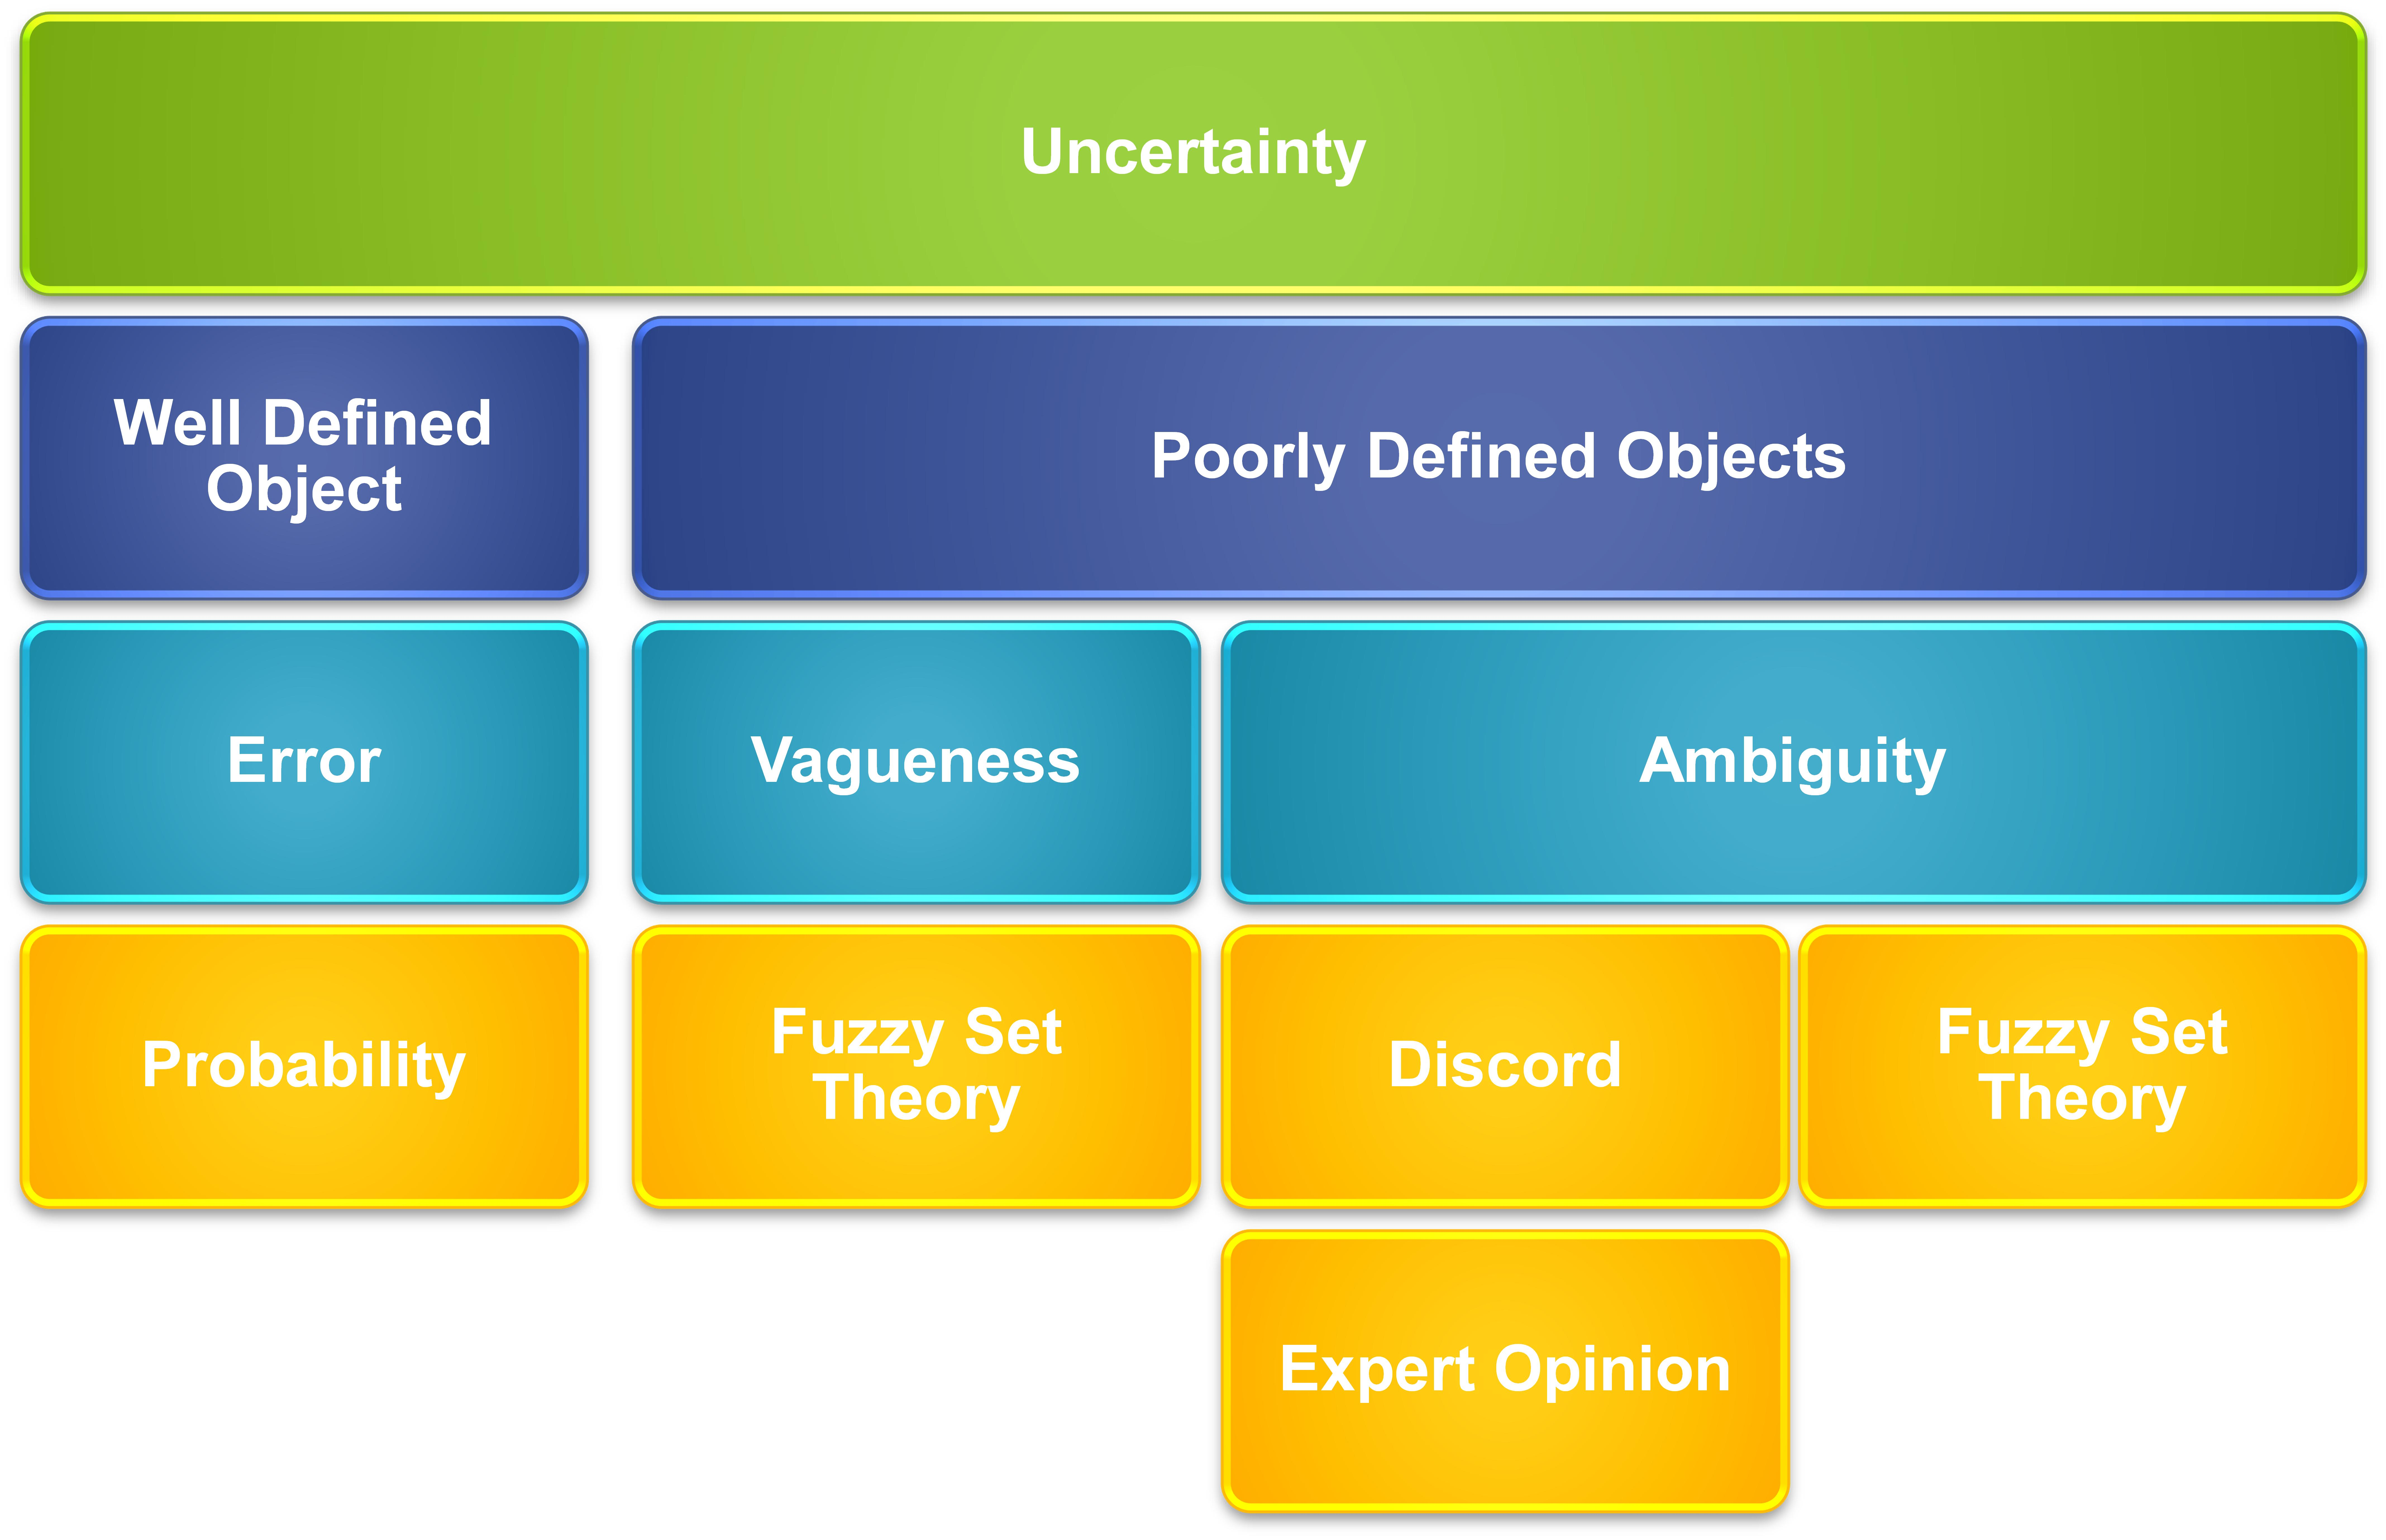
\includegraphics[width=.9\textwidth]{images/uncertainity_type.jpg}
\caption{Types of Uncertainity}
\label{figure:uncertainity_type}
\end{figure}
real-life data analysis shows that the real-life data sources do not produce always certain data. Many real-life data source produces data with error (correctness is not certain). These types of data are named as uncertain data. Figure \ref{figure:uncertainity_type} shows the uncertainty types of real-life dataset. For example location data from GPS sensors mostly produces erroneous data. The correctness of the data is always uncertain. For the uncertainty specialty, these types of data get special attention and concerns to work with. Normal support count is not possible in this type of dataset. This type of database contains data with their corresponding existential probability. That frequent pattern mining of these types of data very much harder. For example, a physician may highly suspicious (but cannot guarantee) that a patient suffers from flu if the patient comes to him having the high fever. The uncertainty of such prediction can be expressed in terms of existential probability. For instance, a patient may have a 90\% likelihood of having the flu, and a 20\% likelihood of having a cold regardless of having the flu. or not. So the probability of having the flu is 0.80 and the probability of having a cold is 0.20. So many real-life dataset may be in between existence and nonexistence. In these situation an item-set \emph{a\textsubscript{i}} can have own existential probability in \emph{a\textsubscript{i}} between 0 and 1($p_i(0<p_i<1)$). Actually understanding uncertain data is the very much tough task but really they exist everywhere. They come with uncertainty to make us confused in terms of poorly defined object, fuzzy sets, ambiguity, error, inherent probability etc. (Figure \ref{figure:uncertainity_type}).\\
There is much real-life scenario where data source always comes with uncertainty. Information gathered from World Wide Web always inherits uncertainty. For example, a system is monitoring user behavior in World Wide Web. It collects data from different websites, extract information and analyze. After the certain period, it finds that one user Mr. X is the citizen of country Y. As he/she can work in Y, there must be a probability that Mr. X is the citizen of Y. There must be a probability value associated with Mr. X's citizenship. So the data is definitely uncertain. Many sensors produce values with some error like 10\% error from GPS data or temperature reading from cell phones.\\
Many approaches has been proposed for finding frequent patterns over uncertain data (U-Apriori ~\cite{u_priori}, UF-growth ~\cite{uf_growth}, UFP-growth ~\cite{ufp_growth} etc.). As the data existence in the database is not certain then normal support calculation is not easy that makes uncertain data very mysterious. So exact frequent pattern finding makes a huge resource sacrifice. For the improvement many approximate algorithms have been proposed (CUF-growth ~\cite{cuf_growth}, CUF\textsuperscript{*}-growth ~\cite{cuf_growth}, PUF-growth ~\cite{puf_growth}). Most of them suffer producing false positives. False positives are those who are not actually frequent but exist in frequent pattern set.

\subsection{Stream Data}
In real-life with the enormous use of the internet, artificial computerized and artificially intelligent devices (smartphones, tablet PC, cars, smart cards etc.) the data source produces a stream millions of data each and every micro second. Storing these data in some storage is out of think nowadays. But this huge data is very valuable for getting interesting information. Moreover, once these data flooded away then can never be found again. The most important property of this kind of dataset is this dataset is unbounded and restless and cannot be defined previously how much data will come. Most recent data is most important but old one is not insignificant and cannot be ignored. This produces a great challenge for researchers to find interesting information from a continuous data stream.\\
For example with the growth of smartphone users much more applications are hitting each and every second. From these usages and data flood finding user behavior to offer some promotional offer for increasing the sale of the online retailer is the very tough job. Another example can be the CCTV video footage of traffic camera. That produces a large number of data flood. In this regard, any sort of any terrorist activity prediction will be very much significant and necessary information for the government. But for a lot of continuous data makes this a very hard job.\\
Stream data makes the database dynamic as there is no limit of data. To find frequent item-set in data stream several algorithms (~\cite{uncertain_01}, ~\cite{uncertain_02}, ~\cite{uncertain_03}, ~\cite{uncertain_04}, ~\cite{uncertain_05}, ~\cite{uncertain_06}) has been proposed. But most are for handling stream but certain data. The uncertainty property makes mining task more complex and complicated the data stream. FP-streaming ~\cite{suf_growth} and  SUF-growth ~\cite{suf_growth} has been proposed for finding frequent, interesting patterns from uncertain and stream data. But these approaches have to compromise runtime efficiency or correctness. However these SUF-growth ~\cite{suf_growth} is an exact approach to finding frequent patterns.
\begin{figure}
\centering
  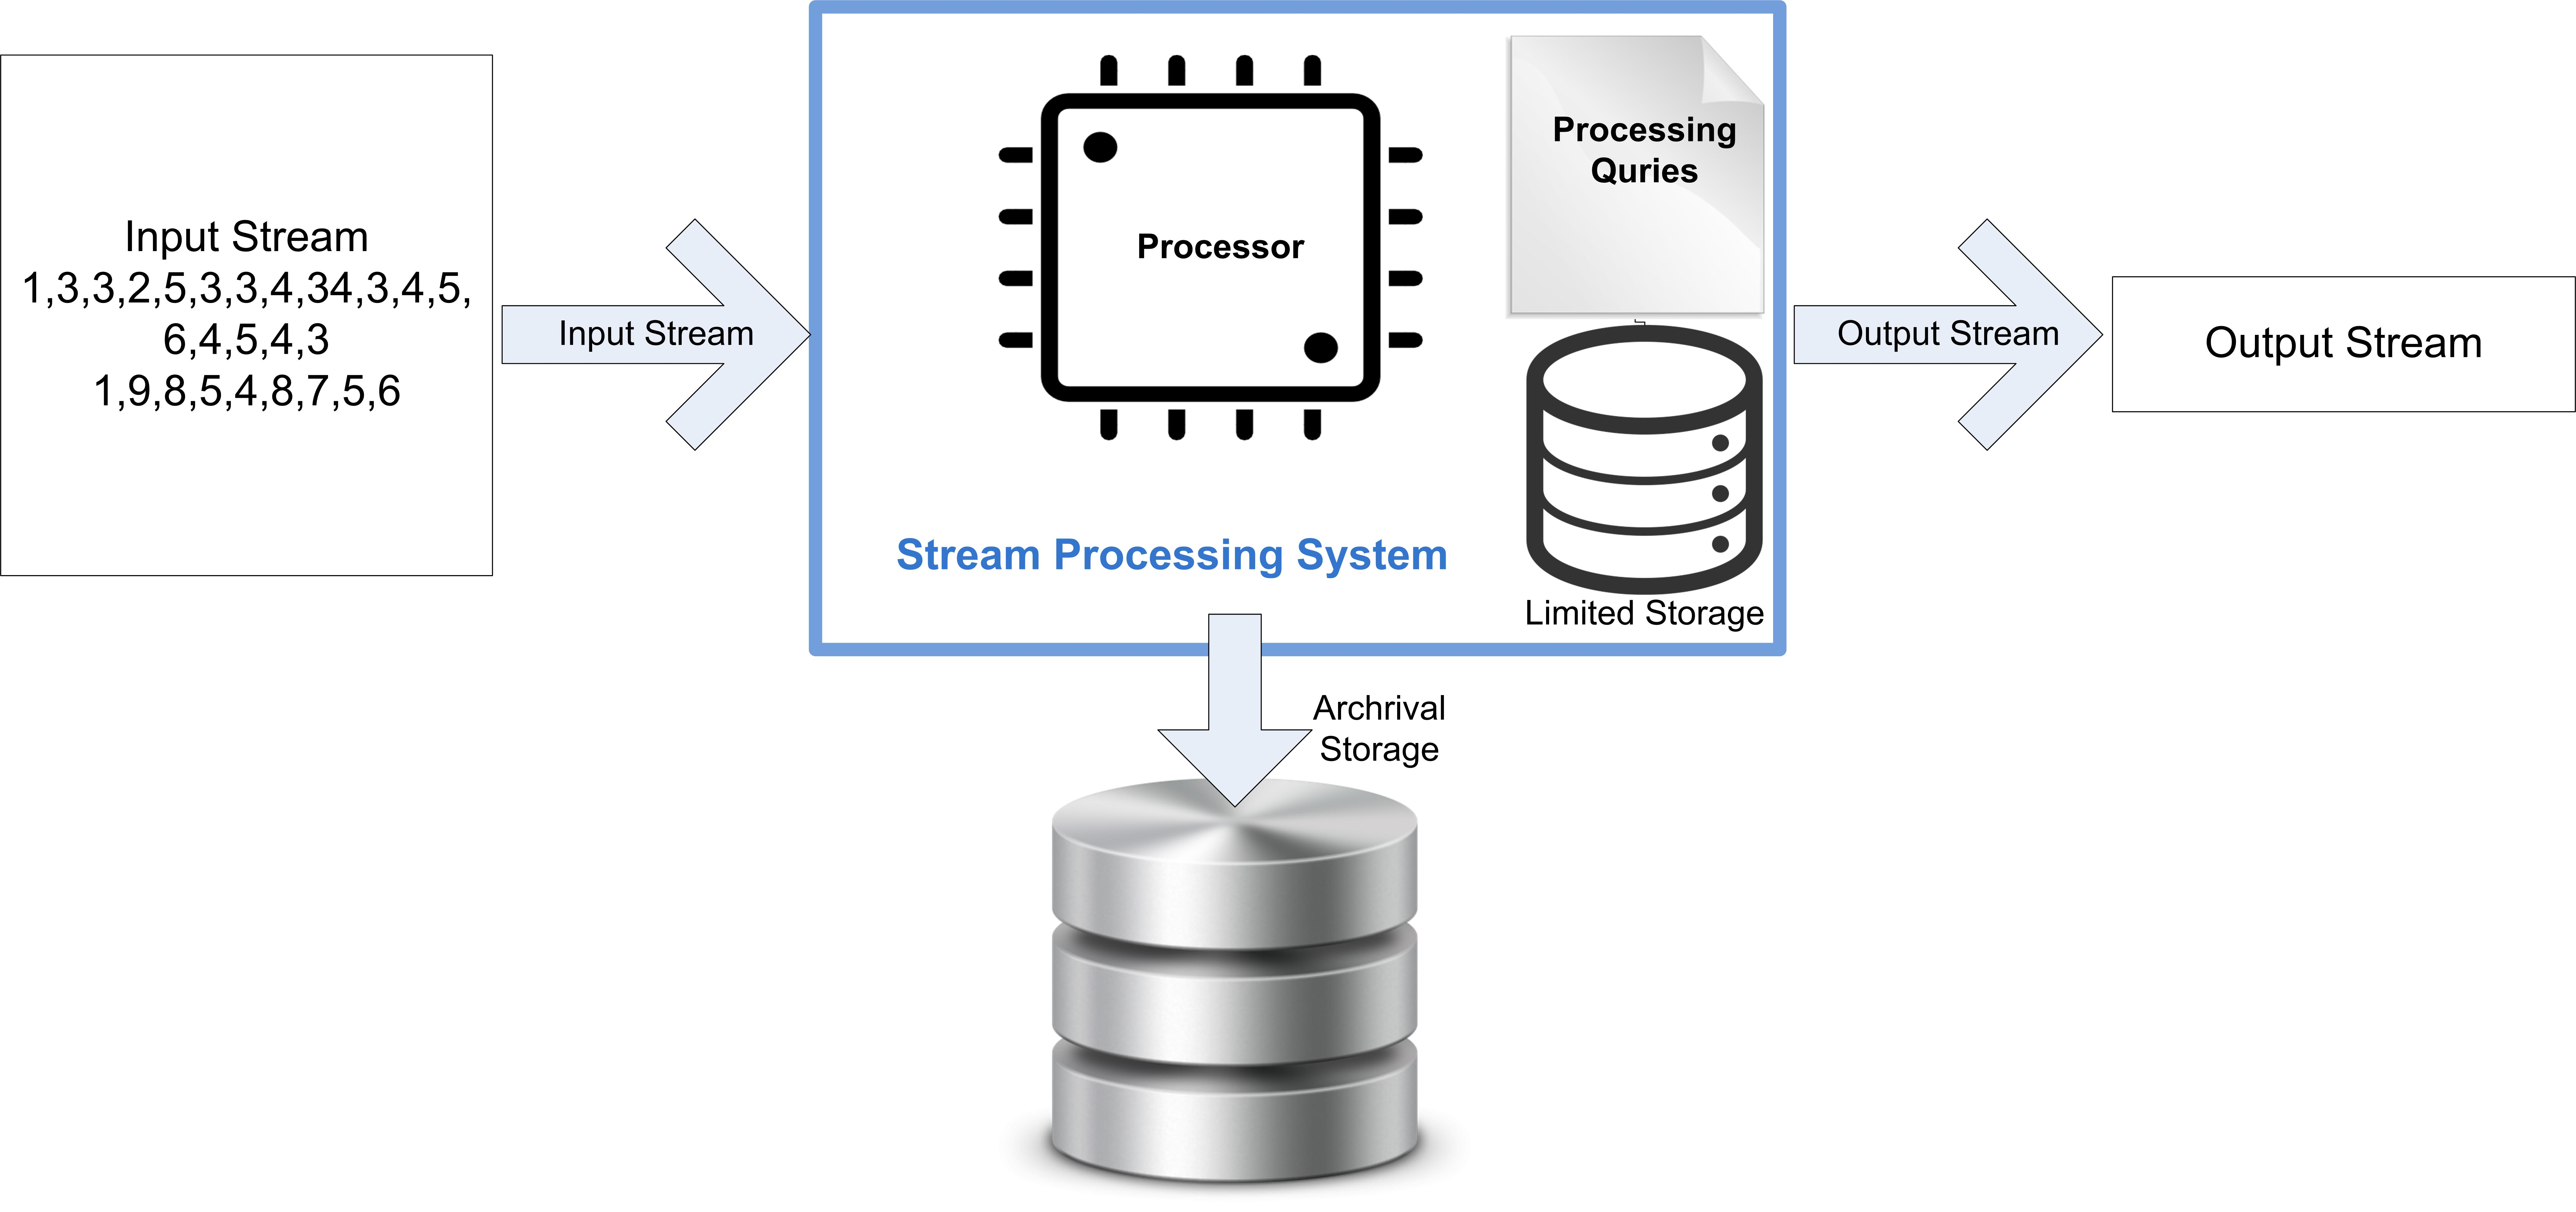
\includegraphics[width=.9\textwidth]{images/stream_data.jpg}
\caption{Types of Uncertainty}
\label{figure:stream_data}
\end{figure}


\section{Motivating Example}
Let us consider \emph{Google Search} ~\cite{google} service as our data source. If we analyze the data coming from source, we find that in each and every millisecond, thousands of people and intelligent devices (e.g. different smart applications of smartphones or PC) are searching in \emph{Google Search}. This search is a continuous process and never stops and we cannot predict earlier when the incoming will be fast and when it will be slow. We can think data incoming like stream. Now if we look at search criteria, we find that \emph{Google Search} service users (both human and machine) are not always searching exactly what she/he/it is looking for. There is much more search with partial key data or key words. For example, when a user searches in Google with key word \emph{Tom Cruise} we cannot surely tell that she/he/it wants to get information of personal life of \emph{Tom Cruise}, next up-coming movie, his movie list, awards he already got or his social activities. We can hardly say, if he is searching for Hollywood movie actor or any other person. This fact makes the task very difficult to find the exact intention of user. The search information is with noise and we do not know exactly that the search key word is with noise or not. So the found information from the \emph{Google Search} is uncertain. The whole scenario indicates to uncertain stream data. \\
Now, if we want to find frequent searched patterns from \emph{Google Search} data then we have to find frequent patterns from these uncertain stream data. Now how can these patterns make us interested, is the first and foremost important question. Let’s consider, after finding frequent patterns, we get information that people are searching for baby food, baby wear for heavy winter, child specialist doctor etc. then we get many important decision. For online retailers the message can be such that if they discount on different products used by babies will increase their sale. For government, now this is heavy winter and much more children are being sick and need to take concerns. This information is really very much valuable.\\
From this scenario it is clear that the gathered information form \emph{Google Search} is very much dynamic and people search criteria can be changed without any prediction and this criteria is always dynamic that makes the frequent patterns finding form found information very much difficult. Again keeping all search information is very much costly as lots of incoming data flow is coming each time. Moreover, the incoming data is not that much precise that we can get any direct conclusion from the search key words.

\section{Aims and Objectives}
Many algorithms have been proposed for mining frequent patterns over certain and uncertain data. Among them in uncertain data mining exact approaches either runtime or the probabilistic models suffers from false positives. Moreover, extraction knowledge from uncertain stream data suffers a lot. The findings are listed briefly below:
\begin{itemize}
    \item Existing algorithms for uncertain data mining suffers either from runtime compromise or the compactness of data storage
    \item In probabilistic uncertain data modeling approach suffers from huge false positives with the frequent item-set.
    \item The proposed data structure in existing approaches for mining uncertain stream data suffers from memory optimization.
    \item Reduction of huge false positives from candidate frequent item-set suffers from runtime inefficiency.
\end{itemize}
To overcome these problems we have followed some objectives. They are given below:
\begin{itemize}
    \item A complete new efficient, robust, scalable approach work with the new data structure that will memory efficient.
    \item Memory and runtime efficient data-structure for both uncertain dynamic database and static databases.
    \item Attach any meta-data with each item of transaction that will make the runtime storage compact as much as possible.
    \item Most recent data is more significant - with this characteristic storing as much as recent data that has more probability to be important.
    \item Giving users the opportunity to keep her/his recent information data as she/he wishes.

\end{itemize}


\section{Our Contribution}
Our key contributions of this paper are given below:
\begin{itemize}
\item We have introduced a prefix value for each item in a transaction which always maintain upper bound of probability. That helps us to make compact pattern tree construction.
\item A new approach \emph{US-tree}, that is very much compact and very memory efficient.
\item A new mining algorithm \emph{USFP-growth}, that is very efficient and reduce mining time surprisingly.
\end{itemize}


\section{Thesis Organization}
	We have carried out the thesis work to consummate the objectives. An outline of rest of the chapters is provided as follows:
	\paragraph{Chapter 2} describes the necessary background study and existing approaches.
	\paragraph{Chapter 3} provides the details of our proposed approach with required analysis.
	\paragraph{Chapter 4} presents the results of experimental results in detail with comparison and analysis.
	\paragraph{Chapter 5} shows several real-life applications for our proposed approach and ends the thesis with a brief conclusion and future scopes.
%\end{document}
 % Introduction
%%
%\documentclass[a4paper,12pt]{book}
%\usepackage{fixltx2e}
%\usepackage{graphicx}	
%\begin{document}
\newpage

\chapter{Background Study and Related Works}
\paragraph{}
In this chapter we describe some related work and provide some background stuffs that are  pertinent to the remainder of this paper.
\section{Data Mining}
What is data mining and frequent pattern mining we have discussed in Chapter 1. Now we discussed related approaches for data mining and frequent pattern mining. There are two common approaches in determining frequent item set. First one is a well known algorithm called Apriori. Apriori is a prior knowledge based  algorithm, that is , if any pattern is not frequent then one of its super-pattern will be frequent.It works in a level wise approach. From the given database in each level it's generate frequent sub-patterns and merges them to propagate the candidates for next level. The second approach is pattern growth e.g., FP-growth method. The FP-Growth methods adopts a divide and conquer strategy as follows: compress the database representing frequent items into a frequent-pattern tree, but retain the itemset association information, and then divide such a compressed database into a set of condition databases, each associated with one frequent item, and mined from the tree. There are no need to generate candidate for next level or no need to generate candidate. Now we given a comparative discussion on this two algorithms or methods. Already we know FP-growth algorithm use divide and conquer strategy approach. That's why in this algorithm needs at most two scans of the database, while the number of database scans for the Apriori algorithm increases with the dimension of the candidate itemsets(Because this approach generate frequent sub-pattern and merges them to generate candidates for next level ). For this reason the performance of FP-growth algorithm is not influenced by the support factor while the performance of the Apriori algorithm decreases with the support factor. Thus prior knowledge based or candidate generating algorithms behave well only for small databases with a large support factor(at least 30\% ).

\section{Uncertain Data Mining}
Data uncertainty is an inherent property in various applications due to reasons such as outdated sources or imprecise measurement. In the age of Big data, uncertainty is one of the defining characteristics of data. Data is constantly growing in volume, variety, velocity and uncertainty. In a large range of applications domains uncertain data is found in abundance.  Today on the web, in sensor networks, within enterprises both in their structured and unstructured sources,in analysis of meteorological trends, of medical behavior of living organisms data are the example of uncertain data. Customer name of a super shop is an real life example of uncertain data.

\begin{figure}[h!]
  \centering
    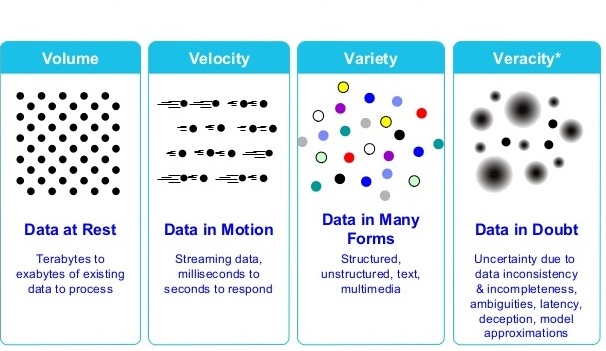
\includegraphics[width=1\textwidth]{images/ra_1}
    \caption{A picture of uncertain data source.}
\end{figure}
In real life we are faced with time series data and features the occurrence of temporal patterns composed of regularity repeating sequences of events, where cyclic activities play a key role.
\begin{figure}
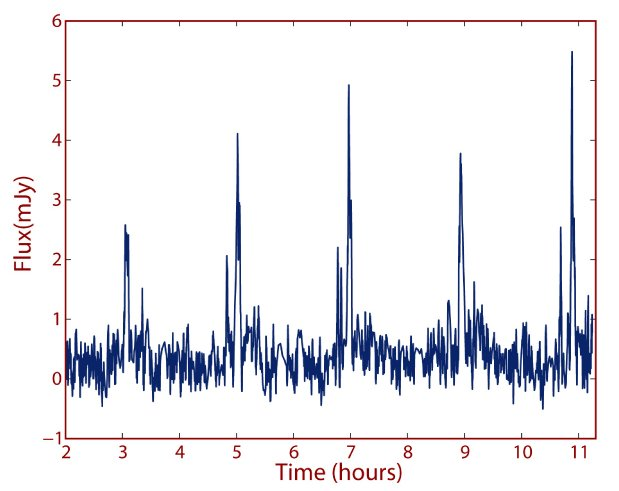
\includegraphics[width=1\textwidth]{images/ra_2}
\caption{A periodic patterns of specific physical medium}
\label{fig:Periodic time series}
\end{figure}
\paragraph{}
An example of periodic time series is given in Figure ~\ref{fig:Periodic time series}, showing the Flux is the presence of a force field in a specified physical medium, or the flow of energy through a surface repetitively occurs. Though consecutive Flux patterns show similar characteristics, they are not equal. It is possible to observe changes in the shape of consecutive periodic patterns that are of significant importance.
\paragraph{}
In the medical domain, physical activity becomes more and more important in the modern society. Nowadays, cardiovascular diseases cover a significant part of a annually occurring affections, which is due to the reduced amount of activity in the daily life. This leads to the research direction of uncertain or probabilistic data. Here, the basic question arises which of these observation in most likely to represent this object. Materialization this likelihood, the observations are associated with probability values; this creates existential dependencies among the observations, as the existence of an observation affects the existence of the other observations of the same object.
\paragraph{}
In the age of big data uncertain data is a common phenomenon.Coping with data uncertainty initiates a need for developing suitable data models and techniques for mining uncertain data. Commonly used models which are used for uncertain data mining are given beneath.
\subsection{Modeling of Uncertain Data}

\begin{figure}[h!]
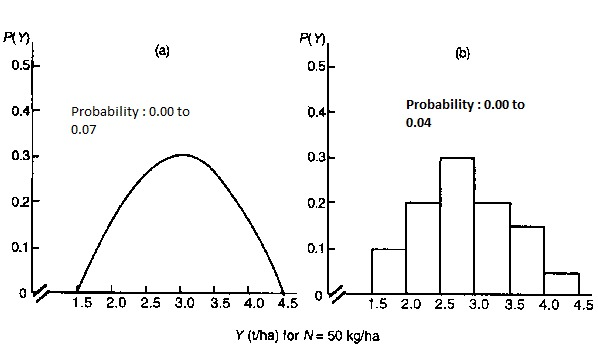
\includegraphics[width=1\textwidth]{images/ra_3}
\caption{Variants of attribute uncertainty}
\label{fig:Uncertainty modeling}
\end{figure}
\subsubsection{Categorization}
There are three main models of uncertain data in databases. In attribute uncertainty, each uncertain attribute in a tuple is subject to its own independent probability distribution. For example, if readings are taken of temperature and wind speed, each would be described by its own probability distribution, as knowing the reading for one measurement would not provide any information about the other.
\paragraph{}
In correlated uncertainty, multiple attributes may be described by a joint probability distribution. For example, if readings are taken of the position of an object, and the x- and y-coordinates stored, the probability of different values may depend on the distance from the recorded coordinates. As distance depends on both coordinates, it may be appropriate to use a joint distribution for these coordinates, as they are not independent.
\paragraph{}
In tuple uncertainty, all the attributes of a tuple are subject to a joint probability distribution. This covers the case of correlated uncertainty, but also includes the case where there is a probability of a tuple not belonging in the relevant relation, which is indicated by all the probabilities not summing to one. For example, assume we have the following tuple from a probabilistic database:
\paragraph{}
$(a, 0.4) | (b, 0.5)$
\paragraph{}
Then, the tuple has 10\% chance of not existing in the database.



\section{Stream Data Mining}
In large application systems or in the age of big data there always needs mining data from continuous or rapid data records. Data Stream Mining is the process of extracting knowledge structures from such kind of data source.A data stream is an ordered sequence of instances that in many applications of data stream mining can be read only once or a small number of times using limited computing and storage capabilities. Example of data source where stream mining is very essential the analysis of meteorological trends, of medical behavior of living organisms, or of recorded physical activity is built on temporally dependent observations or multi observation data, computer network traffic, phone conversations, ATM transactions, web searches, and sensor data.

\paragraph{}
In many data stream mining applications, the goal is to predict the class or value of new instances in the data stream given some knowledge about the class membership or values of previous instances in the data. Data stream mining can be considered a sub-field of data mining stream.
\section{Existing Approaches}
Many algorithms has been developed to mine frequent itemsets from uncertain databases like U-Apriori, UF-growth, UFP-growth, UH-Mine, CUF-growth, CUF-growth, PUF-growth etc.
\subsection{APriori}
Apriori is one of the common algorithm for data mining. It works in a level wise approach based on a prior knowledge. In each level Apriori algorithm generates frequent sub-patterns from the given database and merges them to generate the candidates for next level. That's why this kinds of algorithms called candidates generating algorithm.  Apriori is designed to operate on databases containing transactions (for example, collections of items bought by customers, or details of a website frequentation). Generating frequent sub-patterns it can use large itemset property. The sub-patterns are easily parallelized and it's easy to implement. For those reasons from it's proposed time Apriori is of the frequent used algorithm for data mining.
\paragraph{}
But, some of it's draw back many other algorithms took place over it. The draw back are given below.
\begin{itemize}
 \item Here, number of database scan increases with the dimension of the candidate itemset.
  \item Need transaction databases in memory resident for assumed performance.
\end{itemize}


\subsection{FP growth}
Description
\subsection{U-Priori}
U-Apriori is a  modification of Apriori algorithm which is proposed to handle uncertain data. We already know in Apriori algorithm support count play an important role. Number of databases scan and candidate for next level depends on support count. The modification of Apriori in U-Apriori in support count. Specially, instead of incrementing the support counts of candidate patterns by their actual support, U-Apriori increments the support counts of candidate patterns by their given support count in Apriori. Though U-Apriori come over Apriori to solve support count problem of Apriori but U-Apriori suffers from the following problems:
\begin{itemize}
 \item U-Apriori is a modification of the Apriori algorithm, performance of U-Apriori algorithm for large scale of data because it follows level wise sub-patterns generation and merge to generate candidate for next level. That's why number of databases scan increase with the dimension of itemset.
  \item If the existential probabilities of most items within a pattern I are small, increments for each transaction can be insignificantly small. Consequently, many candidates would not be recognized as infrequent until most transaction were processed.
\end{itemize}
  
\subsection{UF-growth}
Observing outperforms of FP-growth over Apriori UF-growth was proposed for mining uncertain data. We know key to success of FP-growth over Apriori is FP-tree, which is a compact tree structure capturing frequent items within transactions in the databases of precise data. By extracting appropriate tree paths to construct subsequent FP-trees, frequent itemset can be mined. Each tree path represents a transaction. Each node in a tree path captures(i) an item x and (ii) its actual support(i.e, occurrence count of x in that tree path). Tree paths (from the root) are merged if they share the same items(i.e., the captured transaction share the same prefix items). Due to this path sharing, the FP-tree is usually compact. However, when dealing with uncertain data, the situation is different (because each item is associated with an existential probability value). The expected support of any itemset X is the sum of products of existential probability of items within X. Hence, UF-growth uses a UF-tree to capture frequent items within transactions of uncertain data. Each node in an UF-tree captures (i) an item x, (ii) its existential probability value, and (iii) the occurrence count of x in that tree path. By doing so, UF-growth finds all and only those frequent itemsets by computing the expected support of an itemset X (as the sum of products of the captured existential probability values). Tree paths are merged if they share the same items and existential probability values. Consequently, UF-trees may not be as compact as FP-trees.

\subsection{UFP-growth}
To reduce the tree size, UFP-growth groups similar nodes (i.e., nodes with the same x but similar existential probability values) into a cluster. Each cluster of the item x captures (i) the maximum existential probability value of all nodes within the cluster and (ii) the number of existential probability values in each cluster. Depending on the clustering parameter, the resulting tree namely, UFP-tree may be as large as the UF-tree (i.e., no reduction in tree size). On the other hand, if the UFP-tree  is smaller than the UF-tree, then UFP-growth may return approximate results (e.g., with false positives or infrequent itemsets).
\subsection{CUF-growth*}
Description
\subsection{PUF-growth}
To reduce the size of the UF-tree and UFP-tree, the prefix-capped uncertain frequent pattern tree (PUF-tree  structure was proposed, in which important infor- mation about uncertain data is captured so that frequent patterns can be mined from the tree. The PUF-tree  is constructed by considering an upper bound of existential probability value for each item when generating a k-itemset (where k $>$ 1). This upper bound of an item x\textsubscript{r} in a transaction t\textsubscript{j} is called the (prefixed) item cap of x\textsubscript{r} in tj. Thus PUF-tree was compact.
\subsection{SUF-growth}
In this section we propose another algorithm called SUF-growth. SUF-growth algorithm outperforms over UF-streaming algorithm. It improves over UF-streaming by avoiding the aforementioned potential problems for mining frequent itemset from streams of uncertain data. The advantages of SUF-growth over existing others algorithm are given below:
\begin{itemize}
 \item SUF-growth is an exact algorithm. Its means SUF-growth returns only truly frequent itemset. Where UF-streaming returns both true or false frequent itemset.
  \item Its use only minsup. No need to use preMinsup. There also have any problem of finding an appropriate value of preMinsup.
  \item This algorithm does not need UF-stream structure to store the mined itemsets.
  \item Need transaction databases in memory resident for assumed performance. Instead of this its use "delayed" mode for mining. As a result unnecessary computation could be reduced.
\end{itemize}
\paragraph{}
Considering the advantages of SUF-growth over others algorithm there is question. The is how SUF-growth algorithm find frequent itemsets from streams of uncertain data using a new tree structure called SUP-tree. Now we describe about this. We first construct a SUF-tree, and then extract relevant paths from this SUF-tree (which is a global tree) to recursively form smaller UF-trees for projected databases. Due to the dynamic nature and Property 2 of data streams, expected support of items is continuously affected by the arrival of new batches (and the removal of the contents of older batches). Arranging items in frequency-dependent order in the SUF-tree may lead to swapping—which, in turn, can cause merging and splitting—of tree nodes when the global frequencies of items change. Hence, in the SUF-tree, items are arranged according to some canonical order (e.g., lexicographic order), which can be specified by the user prior to the construction of the SUF-tree or the mining process. Consequently, the SUF-tree can be constructed using only one scan of the streams of uncertain data, and the resulting SUF-tree captures the contents of the streams. Moreover, the SUF-tree preserves the usual tree properties:
\begin{itemize}
 \item  The occurrence count of a node is at least as high as the sum of occurrence counts of its children.
  \item The ordering of items is unaffected by the continuous changes in the expected support values of items.
 
\end{itemize}

\section{Summary}
Here is summary.

%\end{document} % Previous Work
%%%
%\documentclass[a4paper,12pt]{book}
%\usepackage{multirow}
%\usepackage{fixltx2e}
%\usepackage{array}
%\usepackage[english]{babel}
%\usepackage{amsmath}
%\usepackage{todonotes}
%\usepackage[]{algorithm2e}
%\begin{document}

\chapter{Our Proposed Approaches}
\lhead{Chapter 3. \emph{Our Proposed Approaches}}

In this section, we will discuss our proposed approach for mining frequent pattern over large uncertain stream data. Stream Data has a special property that it comes and flows away. For this reason, we will always lose data after data stream has flown away. To resolve this, we will propose a sliding window based approach, where we will keep the most recent information in a tree structure because the most recent data is most valuable. Later we will show how the window will slide, remove old data and insert new data in the tree. As, for uncertain data stream each same item in the different transaction has different existential probability, it becomes very difficult to merge (share) these nodes in the tree. This uncertainty property of item makes the tree huge. We have proposed a new \emph{U\textsuperscript{cap}} value for each item that helps to share a single node when constructing the tree which we named as \emph{US-tree}. We will show that our proposed tree \emph{US-tree} will be very compact and very efficient for later mining. Later, we will describe an approach for mining the \emph {US-tree} named \emph{USFP-growth} which is \emph{FP-growth} like approach. Later we will propose a method for filtering and removing false positives generated by our approach in the most probable candidate frequent patterns.

\section{Uncertain Stream Data Properties}
    In this chapter, we will talk about data properties. Our data has two special properties (1) Stream and (2) Uncertainty. For these properties, it becomes very much hard to get valuable and interesting information from data. So first we discuss the data set properties.

    \subsection{Stream Property}
    Stream data are such data those come and go away. They cannot be stored in any patterns. Data streams are continuous and unbounded. This property makes finding patterns so much difficult. As when stream flows away we lose them, we have no choice to store data and scan more than one time we have to find some technique to store valuable information that will help to find valuable information later. For example, table-\ref{table:uncertain_stream_transaction} shows the uncertain stream transaction database. Here \emph{T\textsubscript{1}, T\textsubscript{2}, T\textsubscript{3}, T\textsubscript{4}, T\textsubscript{5}, T\textsubscript{6}, T\textsubscript{7}, T\textsubscript{8}, T\textsubscript{9}} comes one after another and goes away. It may occur that when \emph{T\textsubscript{10}} comes after a long time of \emph{T\textsubscript{4} or T\textsubscript{5} or T\textsubscript{6}} came. So there is no way get \emph{T\textsubscript{4}} when \emph{T\textsubscript{10}} comes. As we are always interested in most recent data, because most recent data are most valuable, we proposed a sliding window based approach that holds the most recent data in our proposed \emph{US-tree} to hold valuable meta information for further valuable frequent pattern extraction.

    \subsection{Uncertainty Property}
    Data is not always precise. Hardware limitations, loss of information during transmission, sampling errors etc. can make precise data uncertain. For this reason the data existence is not for sure. Each time data can comes with a probability value that is called its existential probability. For example, in table-\ref{table:uncertain_stream_transaction}  we can see each transaction having items with item's probability. This value is its existential probability. Let for transaction-\emph{T\textsubscript{2}} there is four items \emph{a(0.9), c(0.6), d(0.5)} and \emph{e(0.2)}. Here \emph{0.9, 0.6, 0.5, 0.2} all are existential probability of corresponding \emph{a, c, d, e}. That means \emph{a's} existential probability is \emph{0.9}. Probability of existence of \emph{a} in those transactions is \emph{0.9}. This property makes mining very much difficult. This property says that in different transaction in a transaction data base same item can have different existential probability. So finding similarity between same items becomes another matter to worry about. For expected support calculation of item becomes very much tough. For expected support calculation equation-\ref{equation:exp_sup} is used.
    %\documentclass{article}
%\usepackage{fixltx2e}
%\begin{document}
\begin{equation}\label{equation:exp_sup}
\emph ExpSup \qquad = \qquad \sum_{i = 0}^{UDB} [\prod_{x \in I } p(x , t_i)]
\end{equation}
\begin{center}


\textbf{\emph {where,}}\\ 
\begin{itemize}
\item
\textbf{\emph {I}} is itemset,
\item
\textbf{\emph { p(x, ti)}} is existential probability value for any item \textbf{\emph {x}} in transaction \textbf{\emph {t\textsubscript{i}}} 
\item
\textbf{\emph {UDB}} is an uncertain database.

\end{itemize}
\end{center}
%
%\end{document}
    From this equation we can see that calculation of support is not that easy and straight forward like certain data. Certain data support is calculated just counting the total existence of that items in the transaction were as for uncertain data it depends on its existential probability. It may occur that some data set exists many times in a transaction database but with a low probability, so ultimately the data must not be frequent. For example, if we want to find the support of \emph{ae} of table-\ref{table:uncertain_stream_transaction} then we need to do the following calculation. For \emph{T\textsubscript{2}} $0.9*0.2=0.18$, \emph{T\textsubscript{2}} $0.9*0.1=0.09$, \emph{T\textsubscript{3}} $0.0$, \emph{T\textsubscript{4}} $0.0$, \emph{T\textsubscript{5}} $0.0$, \emph{T\textsubscript{6}} $0.9*0.3=0.27$, \emph{T\textsubscript{7}} $0.1*0.2=0.02$, \emph{T\textsubscript{8}}=$0.0$ and \emph{T\textsubscript{9}}=$0.0$.$Sup_{ae} =Sup_{ae(T_1)}+Sup_{ae(T_2)}+Sup_{ae(T_3)}+Sup_{ae(T_4)}+Sup_{ae(T_5)}+Sup_{ae(T_6)}+Sup_{ae(T_7)}+Sup_{ae(T_8)}+Sup_{ae(T_9)}=0.18+0.09+0.0+0.0+0.0+0.27+0.0+0.02+0.0+0.0=0.54$ So if \emph{minimum support is $0.9$} than \emph{ae} is not frequent but \emph{ae} exists four times in the transaction. So it makes very much difficult to find which a pattern is important or not.
    
    
\section{Preliminaries}
    \paragraph{Definition-1 Uncertain Frequent Pattern: }
    Given DB = \emph{\{T\textsubscript{1}, T\textsubscript{2}, T\textsubscript{3} . . . T\textsubscript{N} \}} , an uncertain database with \emph{N} transactions where minimum expected support threshold is $\delta$. The problem is to mine frequent item-sets \emph{FI} $\subset$ DB, where $ExpSup(FI_i) \geq \delta $ and $FI_i \in FI$.
    
    \paragraph{Definition-2 Batch: }
    A group of consecutive transactions from a transaction \emph{DB}inserted in \emph{US-tree} at a time. Let table-\ref{table:uncertain_stream_transaction} batch size = \emph{3}. \emph{T\textsubscript{1}, T\textsubscript{2}, T\textsubscript{3}} is one batch and its batch-1. Then next three \emph{T\textsubscript{4}, T\textsubscript{5}, T\textsubscript{6}} is one batch and its batch-2.
    
    \paragraph{Definition-3 Window: } Window is the size of consecutive batchs one \emph{US-tree} can hold. Let table-\ref{table:transaction_batch} be an example of grouped transaction and batch number tagged. So for window size \emph{2} The in a certain time batch-1 and batch-2 will create a window. Then after some times when batch-3 comes then batch-2 and batch-3 will create the next window.
    
    \paragraph{Definition-4 U\textsuperscript{cap} :}
    The following equation is for \emph{U\textsuperscript{cap}}    calculation.
    %\documentclass{article}
%\usepackage{amsmath}
%\begin{document}
\begin{equation}\label{equation:cap}
\text{\emph{U\textsuperscript{cap}}}(X_r) =\begin{cases}
				P(X_1), & \text{if $ h = 1$}\\
				P(X_r)*M, & \text{if $ h > 1$}
             
\end{cases}
where, M=max_{1\leq q\leq h}P(X_q)
\end{equation}
%\end{document}
    For transaction \emph{DB} example in table-\ref{table:uncertain_stream_transaction} for \emph{T\textsubscript{1}}, \emph{U\textsuperscript{cap}} of \emph{a{0.9}} is $0.9$ as a is the first item. For \emph{c(0.6)} \emph{U\textsuperscript{cap}} is $0.9*0.6=0.45$, \emph{d(0.50)} \emph{U\textsuperscript{cap}} is $0.9*0.5=0.45$ and \emph{e(0.2)} \emph{U\textsuperscript{cap}} is $0.9*0.2=0.18$. \emph{U\textsuperscript{cap}} is the upper bound of existential probability. As we are taking the max of all previous items coming in a particular order all items or item sets having existential probability must be less than or equal \emph{U\textsuperscript{cap}}. that is $\forall(i,j)\{ P(I_i)*P(I_j)\leq U_{cap}(I_j)\}$ where $i < j$. So support must be less than or equal \emph{U\textsubscript{cap}}.\\
    Calculated \emph{U\textsuperscript{cap}} should be the upper bound of two item's existential probability because we have taken the maximum value of item that has come earlier. So, by two item set support that can have maximum support value, is \emph{U\textsuperscript{cap}} value. Item set having \emph{U\textsuperscript{cap}} less than minimum support must frequent. Though this may cause some false positives but it is for sure that no false negative will insert into this. 
    %\documentclass{article} 
%\usepackage{graphicx}  
%\usepackage{multirow}
%\usepackage[table]{xcolor}
%\usepackage{fixltx2e}
%\usepackage{array}
%
%\begin{document}
\begin{table}[t]
\centering

\begin{tabular}{|c|c|c|c|c|c|}
\hline
& No & \multicolumn{4}{c|}{Items in Transaction} \\ \hline \hline
\multirow{3}{*}{Batch 1}	&	T\textsubscript{1} & a(0.9) & c(0.6) & d(0.5) & e(0.2)\\
							&	T\textsubscript{2} & a(0.9) & b(0.4) & e(0.1) & --    \\
							&	T\textsubscript{3} & a(0.2) & c(0.9) & d(0.7) & --    \\\hline
\multirow{3}{*}{Batch 2}	&	T\textsubscript{4} & b(0.3) & c(0.9) & -- & --\\
							&	T\textsubscript{5} & a(0.1) & b(0.3) & c(0.9) & --    \\
							&	T\textsubscript{6} & a(0.9) & e(0.3) & -- & --        \\\hline
\multirow{3}{*}{Batch 3}	&	T\textsubscript{7} & a(0.1) & d(0.6) & e(0.2) & --    \\
							&	T\textsubscript{8} & a(0.1) & c(0.2) & f(0.6) & --    \\
							&	T\textsubscript{9} & c(0.2) & d(0.9) & f(0.6) & --    \\\hline
							
\multirow{3}{*}{Batch 4}	&	T\textsubscript{10} &  --  &  --  &  --  & --    \\
							&	T\textsubscript{11} &  --  &  --  &  --  & --    \\
							&	T\textsubscript{12} &  --  &  --  &  --  & --    \\\hline
\end{tabular}
\caption{Uncertain Stream Transaction Data Divided into Batch}
\label{table:transaction_batch}
\end{table}


%
%\end{document}
	
    \paragraph{Definition-5 : False Positive: } False positive is pattern which exists in frequent pattern set but actually not frequent. Probabilistic approach for mining frequent patterns sometimes generates false positive patterns. Let, \emph{\{a, ab, b, bc, c, d, cd, de, cde\}} be frequent pattern set found from any mining algorithm. Here, \emph{\{a, ab, b, bc, c, d, cd, de\}} is actual frequent pattern set, but \emph{\{ cde\}} is not frequent, then \emph{\{ cde\}} is false positive. Exact mining algorithms do not produces false positive patterns.
    
	\paragraph{Definition-5 : False Negative: } False negative is pattern which does not exist in frequent pattern set but actually frequent. Probabilistic mining approaches sometimes produce false negative patterns. Let, \emph{\{a, ab, b, bc, c, d, cd, de, cde\}} be found frequent pattern set by any mining algorithm. Later it is found that, \emph{\{b\}} is actually frequent but not in frequent pattern set. So, \emph{\{ b\}} is false negative pattern. Exact mining algorithm does not generate false negative patterns.
	
	\paragraph{Theorem 1: } Let X be a $k$-itemset in transaction $T_j$ (where $k > 1$). The existential probability of any of its non-empty proper subset Y that shares the same suffix $x_r$ as X (i.e., $Y \subset X \subseteq T_j$) is always less than or equal to $U^{cap}(X_r$, $T_j)$.\\
		\emph{\textbf{Proof:}}\\
		Let'
		$T_j = \{X_1$, $X_2$, $X_3$ . . . , $X_r$, . . . , $X_h$\}
		$X = \{X_s$, . . . , xr\} be a k-itemset in $T_j$
		$Y = \{X_t$, . . . , $X_r$\} be a $k_1$-itemset (where $k_1 < k$) and a proper subset of $X$ (i.e. $Y \subset X \subseteq T_j$).\\
		$\prod_{(X \epsilon Y)\bigwedge (X\neq X_r)}P(X,T_j) \leq max_{1 \leq q \leq r-1}$ because $0< P(X, T_j)\leq 1$. So,\\
		 $P(Y,T_j)=P(X_r,T_j)*\prod_{(X \epsilon Y)\bigwedge (X\neq X_r)}P(X,T_j)$\\
		 $\leq P(X,T_j)*max_{1 \leq q \leq r-1}=U^{cap}(X$, $T_j)$
 
\section{Mining Frequent Patterns from Uncertain Databases}
    Our proposed algorithm is divided into five parts. (1) Grouping transactions into batches and window and giving each item in a transaction a prefix value is called \emph{U\textsuperscript{cap}}. (2) Insert transaction into \emph {US-tree}. (3) Sliding the \emph {US-tree} (4) mining the \emph {US-tree} with \emph{USFP-growth} algorithm and (5) Eliminating false positive (not frequent but exists infrequent item set) . For simulating our approach we consider Table~\ref{table:uncertain_stream_transaction} as uncertain stream transaction data. For this simulation, we consider window size as 2 and batch size 3. That means 3 transactions creates a batch and 2 batches create a window. After completing window construction (inserting batch 1 and 2), the \emph {US-tree} will be full. When new batch comes we slide the window. That means we remove oldest batch batch-1 and put batch-2 as the old batch. Then insert new batch in the tree as batch-3. So for window size 2 the tree always contains at most 2 batches. Thus, the tree always holds the latest information. In next subsections, we will elaborately explain our approach of every step.

    \subsection{Preparation}
    %\documentclass{article} 
%\usepackage{graphicx}  
%\usepackage{multirow}
%\usepackage[table]{xcolor}
%\usepackage{fixltx2e}
%\usepackage{array}
%
%\begin{document}
\begin{table}
\centering

\begin{tabular}{|l|l|l|l|l|l|}
\hline
	Batch No& No & \multicolumn{4}{c|}{Items in Transaction} \\ \hline \hline
	\multirow{3}{*}{Batch 1}	&	T\textsubscript{1} & a(0.9) & c(0.54) & d(0.45) & e(0.18)			\\\cline{2-6}
								&	T\textsubscript{2} & a(0.9) & b(0.36) & e(0.09) & --			\\\cline{2-6}
								&	T\textsubscript{3} & a(0.2) & c(0.18) & d(0.63) & --			\\\hline
	\multirow{3}{*}{Batch 2}	&	T\textsubscript{4} & b(0.3) & c(0.27) & 	--     & --	\\\cline{2-6}
								&	T\textsubscript{5} & a(0.1) & b(0.03) & c(0.27) & --  			\\\cline{2-6}
								&	T\textsubscript{6} & a(0.9) & e(0.27) & --	   & --  			\\\hline
	\multirow{3}{*}{Batch 3}	&	T\textsubscript{7} & a(0.1) & d(0.06) & e(0.12) & --	\\\cline{2-6}
								&	T\textsubscript{8} & a(0.1) & c(0.02) & f(0.12) & --   			\\\cline{2-6}
								&	T\textsubscript{9} & c(0.2) & d(0.09) & f(0.54) & --   			\\\hline
								
	\multirow{3}{*}{Batch 4}	&	T\textsubscript{10} &  --  &  --  &  --  & --    				\\\cline{2-6}
								&	T\textsubscript{11} &  --  &  --  &  --  & --    				\\\cline{2-6}
								&	T\textsubscript{12} &  --  &  --  &  --  & --    				\\\hline
	\end{tabular}
\caption{Window and Batch of Table\ref{table:uncertain_stream_transaction}}
\label{table:prefix_assigned}
\end{table}


%
%\end{document}
    In this section we will describe the batch and window grouping and the prefix value \emph{U\textsuperscript{cap}} calculation. First we calculate batch and window calculation and grouping our transaction data. As we describe earlier for the example Table-\ref{table:uncertain_stream_transaction} easy simulation we take batch size as \emph{$3$} and window size as \emph{$2$}. So first \emph{$3$} transactions \emph{T\textsubscript{1}}, \emph{T\textsubscript{2}} and \emph{T\textsubscript{3}} are grouped and labeled as \emph{Batch-1}. Then next \emph{$3$} \emph{T\textsubscript{4}}, \emph{T\textsubscript{5}} and \emph{T\textsubscript{6}} are grouped together and labeled as \emph{Batch-2}. Next \emph{$3$} \emph{T\textsubscript{7}}, \emph{T\textsubscript{8}} and \emph{T\textsubscript{9}} are grouped together and labeled as \emph{Batch-3}. Thus the consecutive next \emph{$3$} transaction should be grouped as batch and ready to be inserted into \emph{US-tree}. As our window size is $2$, after inserting two batches into the \emph{US-tree} the window will be completed. Before inserting next batch \emph{Batch-3} we need to remove \emph{Batch-1}(oldest one) from tree and move \emph{Batch-2} to \emph{Batch-1 's} position and then insert new batch, \emph{Batch-3}. Thus the latest information is inserted and kept into the \emph{US-tree}. table-\ref{table:transaction_batch} shows the window and batch grouped for stream transaction example table-\ref{table:uncertain_stream_transaction}.
    For this calculation we earlier proposed an equation-\ref{equation:cap}. From this equation we can create \emph{U\textsuperscript{cap}} for each item in a transaction. To calculate one transaction, for each item in a transaction, if item is the first item in a transaction than item's existential probability is its \emph{U\textsuperscript{cap}} value, otherwise item's \emph{U\textsuperscript{cap}} is max of previous items existential probability multiplied by item's  own existential probability. For example, let Table-\ref{table:transaction_batch} T1 is \emph{a(0.9), c(0.6), d(0.5), e(0.2)}. \\
    In this transaction item \emph{a(0.9)} is the first item. So its \emph{U\textsuperscript{cap}} is 0.9.\\
    For second item, \emph{c(0.60)} previous item is only \emph{a(0.90)}. So c's $\emph{U\textsuperscript{cap}} = 0.9*0.6 = 0.54$. \\
    For third item, \emph{d(0.50)} there are two items before it, \emph{a(0.9)} and \emph{c(0.6)}. Among them \emph{a} has max existential probability, that is \emph{0.9}. So \emph{d's } $\emph{U\textsuperscript{cap}} = 0.9*0.5 = 0.45$.\\
    For fourth item \emph{e(0.2)} there are three items before it, \emph{a(0.9)} ,\emph{c(0.6)} and \emph{d(0.5)}. Among them \emph{a} has max existential probability is \emph{0.9}. So \emph{e's}  $\emph{U\textsuperscript{cap}} = 0.9*0.2 = 0.45$. Thus we can calculate each item's \emph{U\textsuperscript{cap}} value for a transaction. For easier understanding we have calculated all the item's \emph{U\textsuperscript{cap}} of Table-\ref{table:transaction_batch} and put into Table-\ref{table:prefix_assigned}.
    
    
    
    \subsection{US-tree Construction}
    In this section we will describe about our tree construction \emph{US-tree}. We have described earlier about our batch and window. A batch should be inserted into the tree in its own window slot. After inserting all batches, the window will be complete and be ready to mine. We said earlier section that our tree will be very compact. For this we have proposed an approach for sharing nodes. For sharing same tree nodes two items with same id and order should not care about own existential probability. If item is already in the tree with same id then two items should share the node. Thus the tree will be very compact. When inserting an item in the tree the \emph{U\textsuperscript{cap}} of the tree should be updated by adding the prefix value of the node. Thus each batch should be inserted into the tree. The algorithm is given in the algorithm section Algorithm-\ref{algorithm:tree_construction}.
    %\documentclass{article}
%\usepackage{graphicx}
%\usepackage{caption}
%\usepackage{subcaption}
%
%\begin{document}
\begin{figure}[!tbp]
  \centering
	\fbox{  
	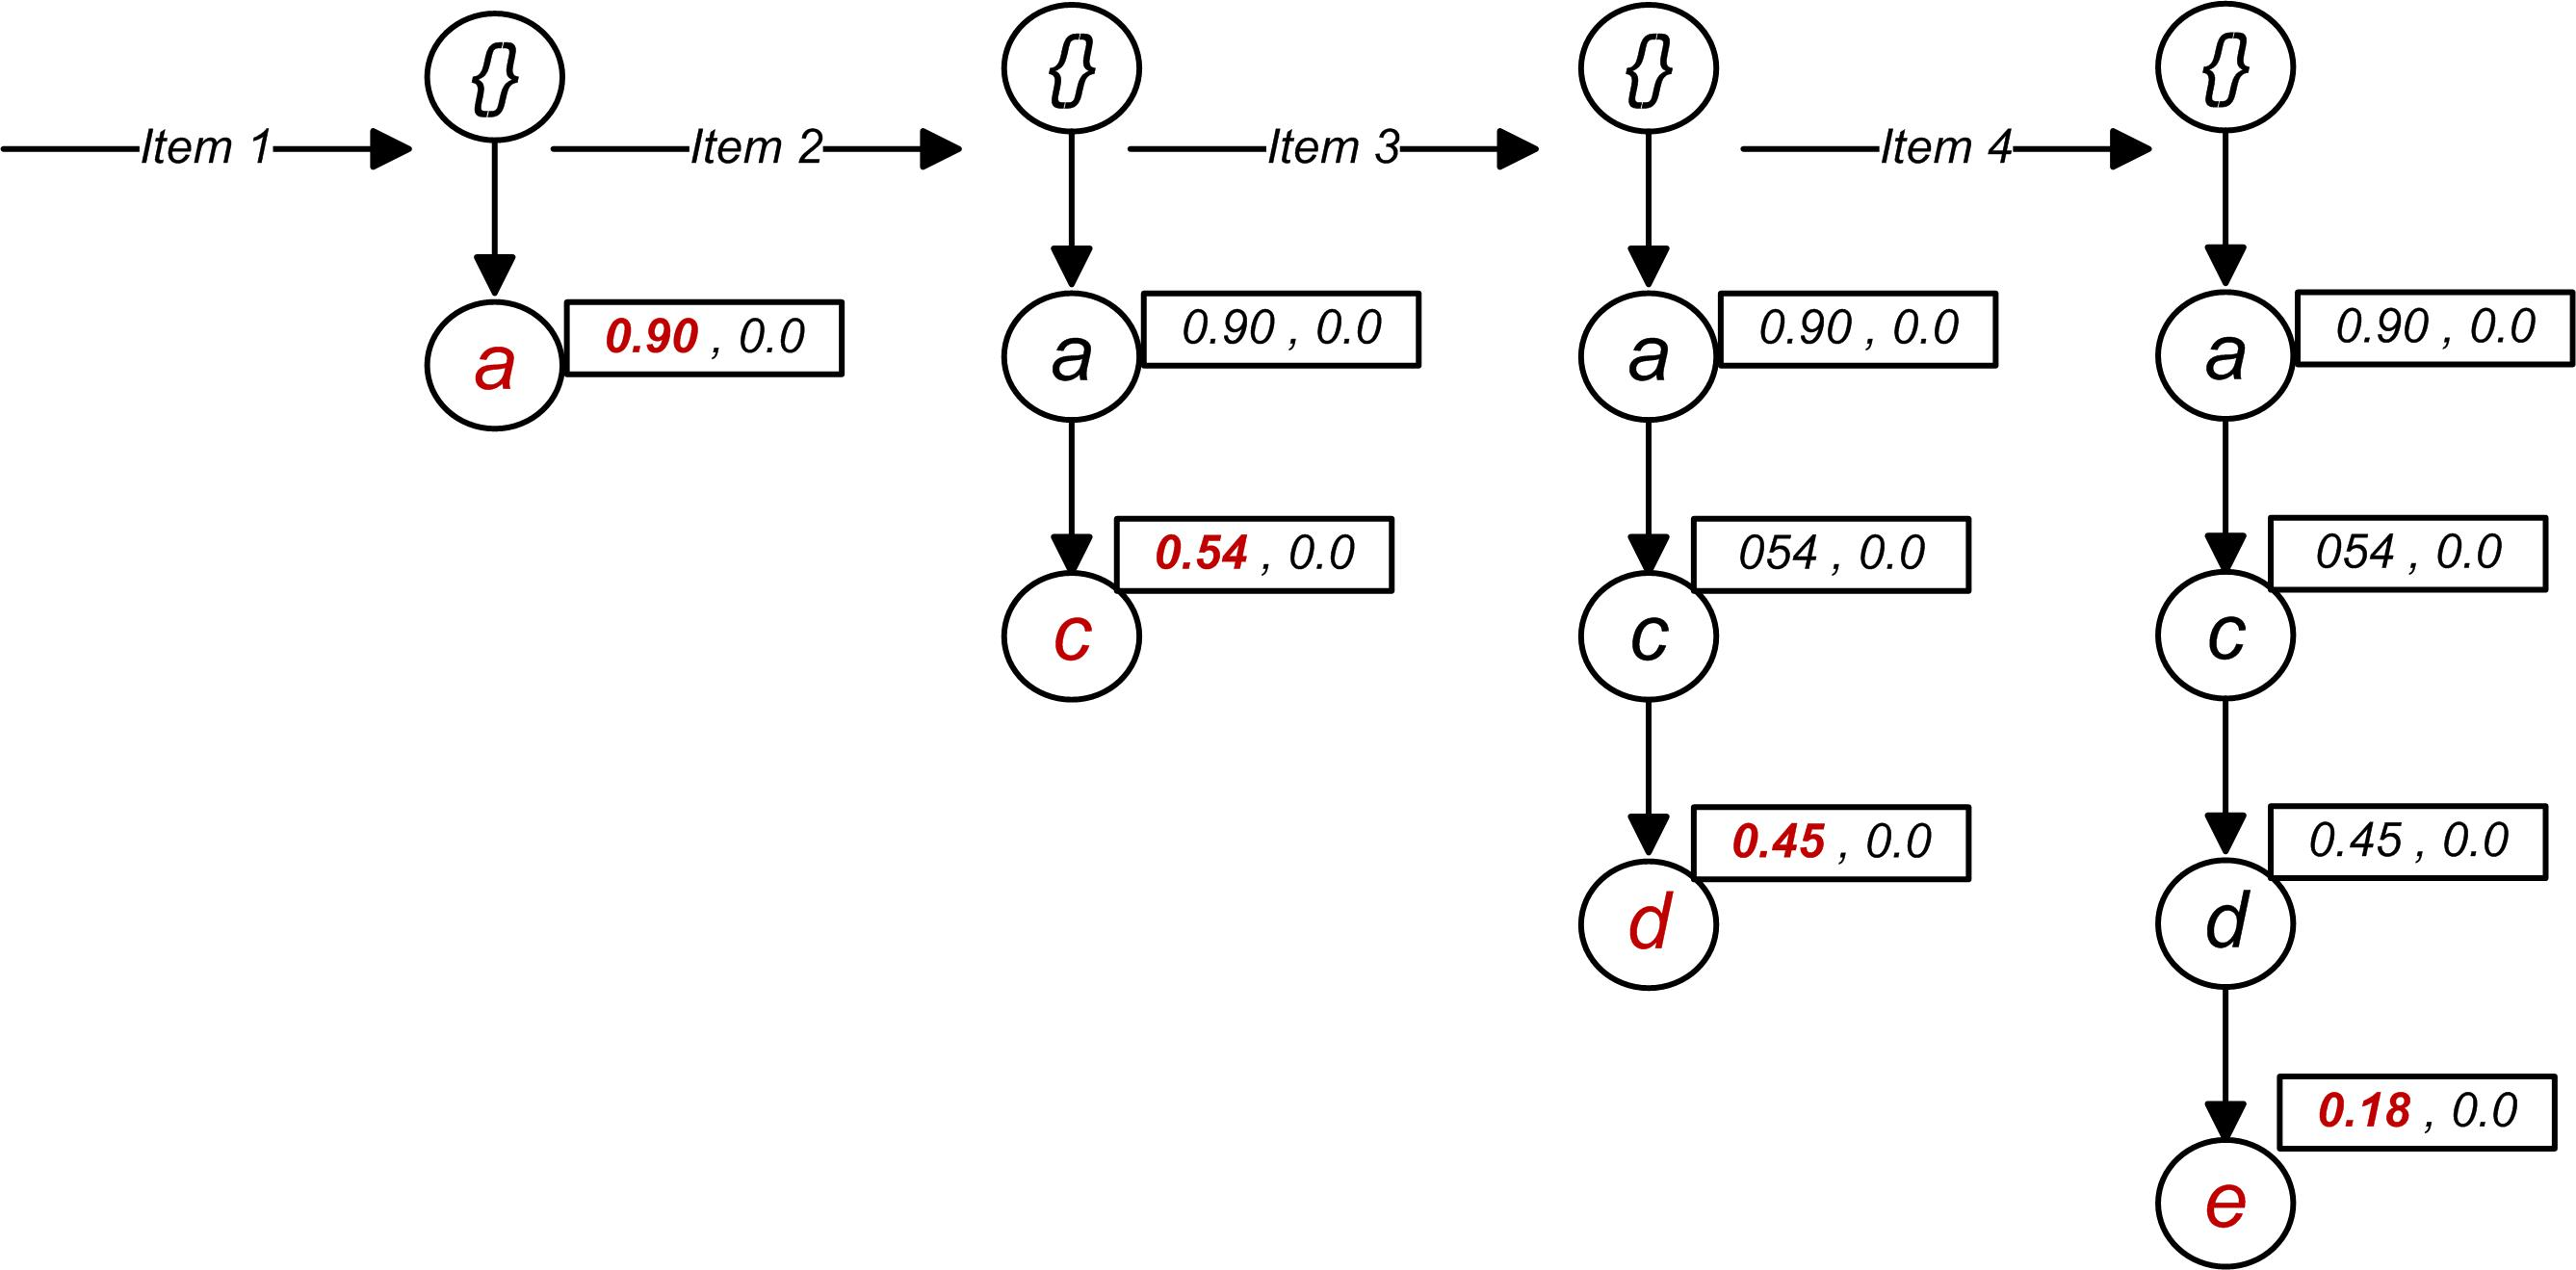
\includegraphics[width=.8\textwidth,height=5cm]{images/sim_01.jpg}  
	}
	\caption{Inserting \emph{T\textsubscript{1}} into \emph{US-tree}}
	\label{figure:t1}
\end{figure}
\begin{frame}

\begin{figure}[!tbp]
  \centering
	\fbox{  
	 	\begin{subfigure}[b]{0.40\textwidth}
	 	\centering
	    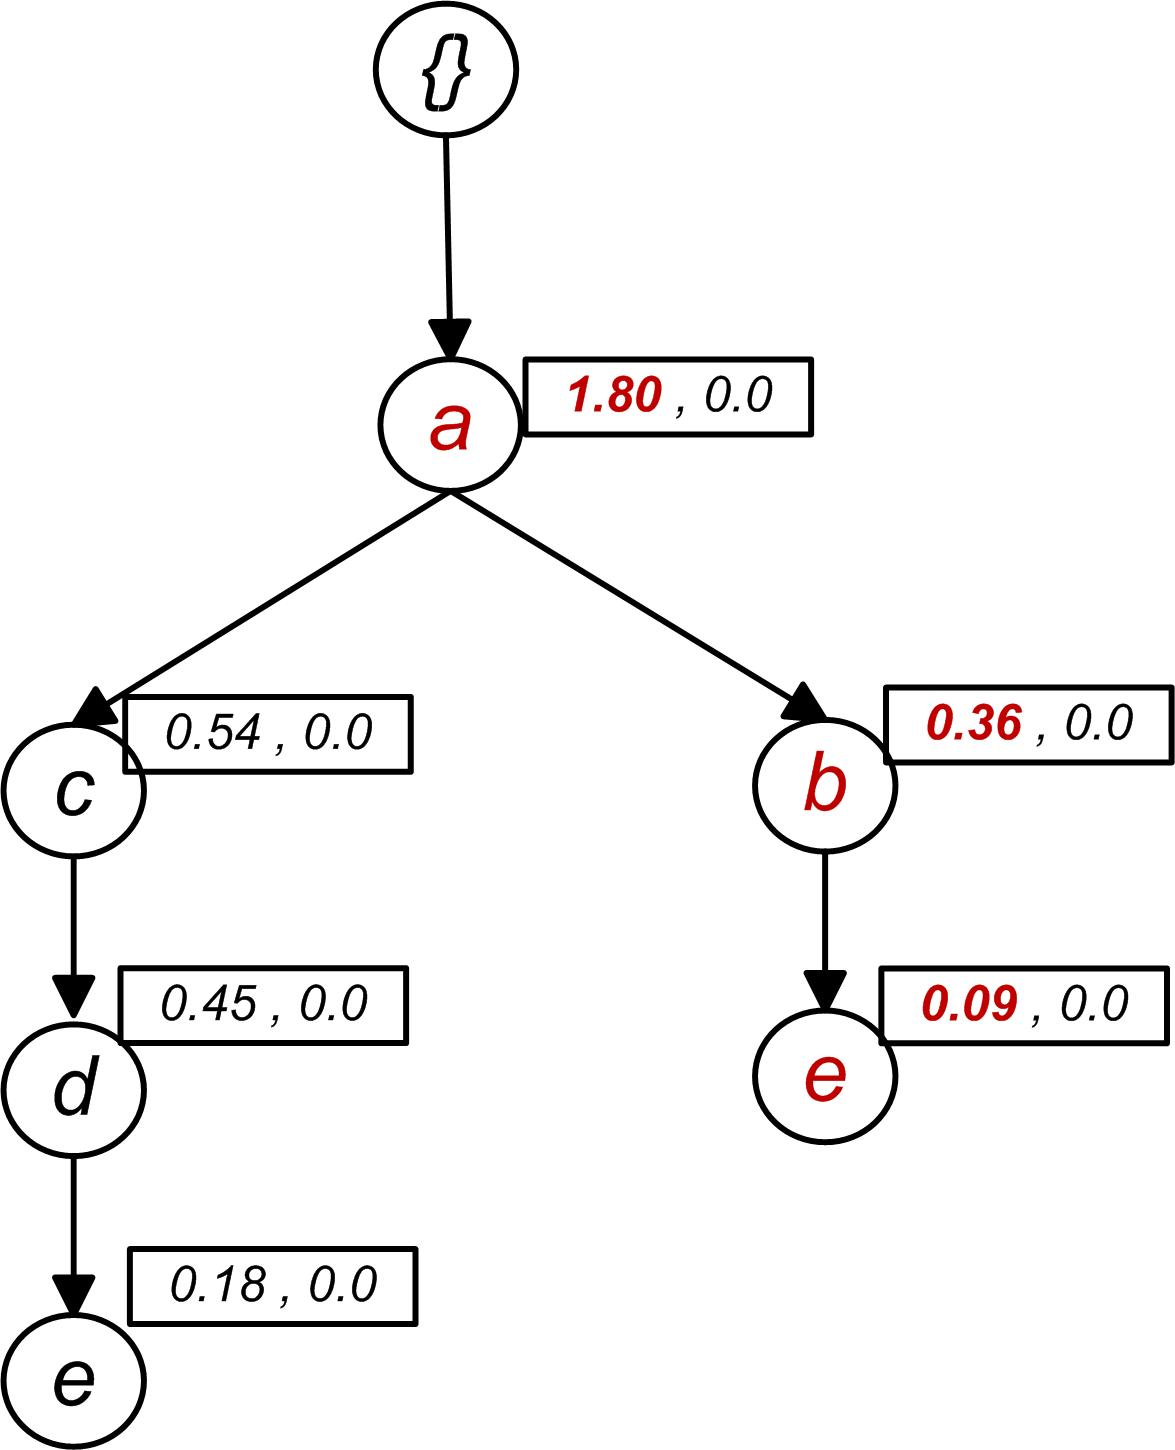
\includegraphics[width=.8\textwidth,height=4cm]{images/sim_02.jpg}
	    \caption{T\textsubscript{2}}
		\end{subfigure}
	  
	 	\begin{subfigure}[b]{0.40\textwidth}
	 	\centering
	    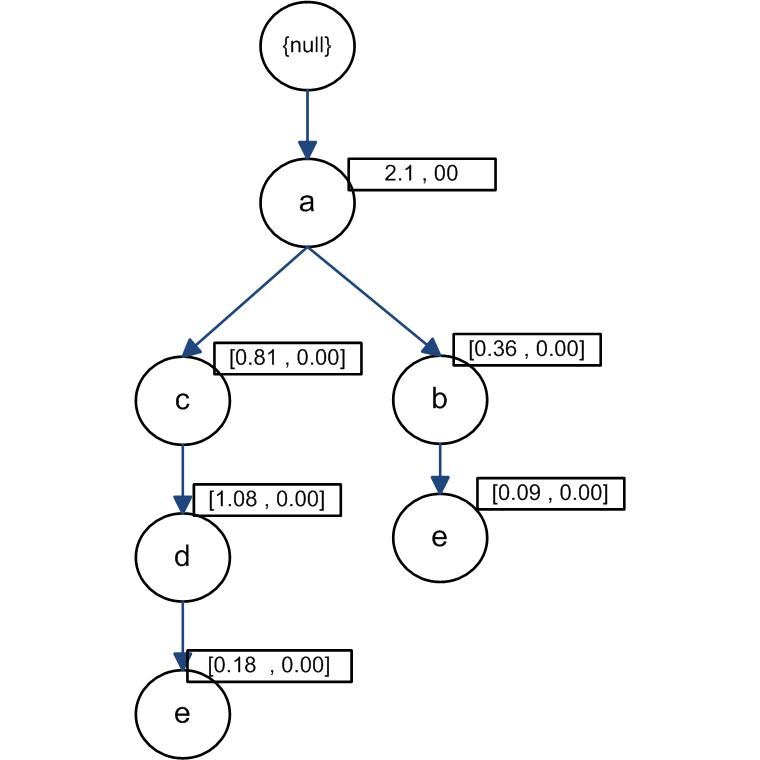
\includegraphics[width=.8\textwidth,height=4cm]{images/sim_03.jpg}
	    \caption{T\textsubscript{3}}
		\end{subfigure}
	}
 \caption{Inserting \emph{T\textsubscript{2}} and \emph{T\textsubscript{3}} in \emph{US-tree}}
 \label{figure:t23}
\end{figure}
\end{frame}
\begin{frame}

\begin{figure}[!tbp]
  \centering
	\fbox{  
	 	\begin{subfigure}[b]{0.22\textwidth}
	 	\centering
	    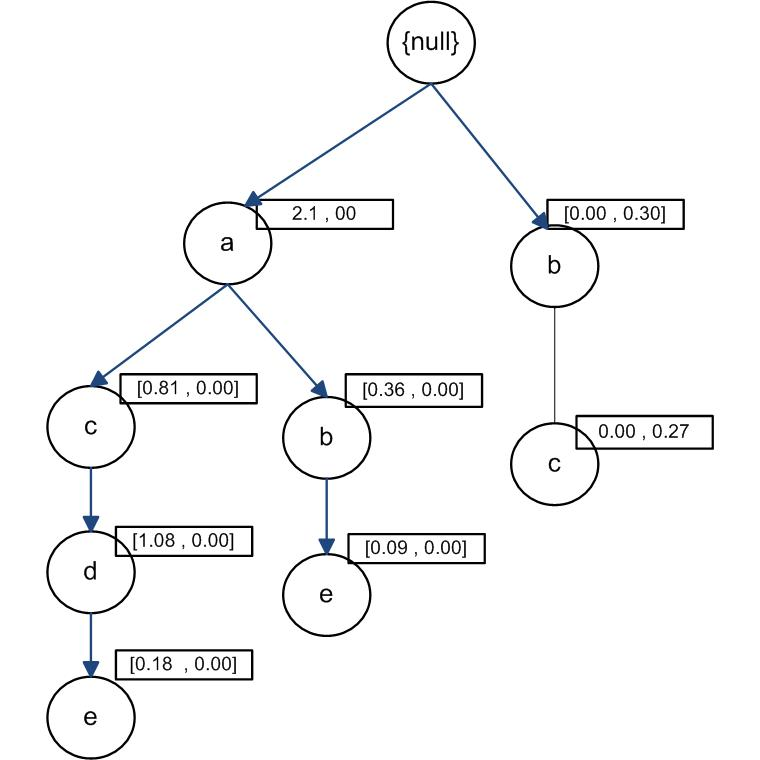
\includegraphics[width=\textwidth,height=4.0cm]{images/sim_04.jpg}
	    \caption{T\textsubscript{4}}
		\end{subfigure}
	 
	 	\begin{subfigure}[b]{0.27\textwidth}
	 	\centering
	    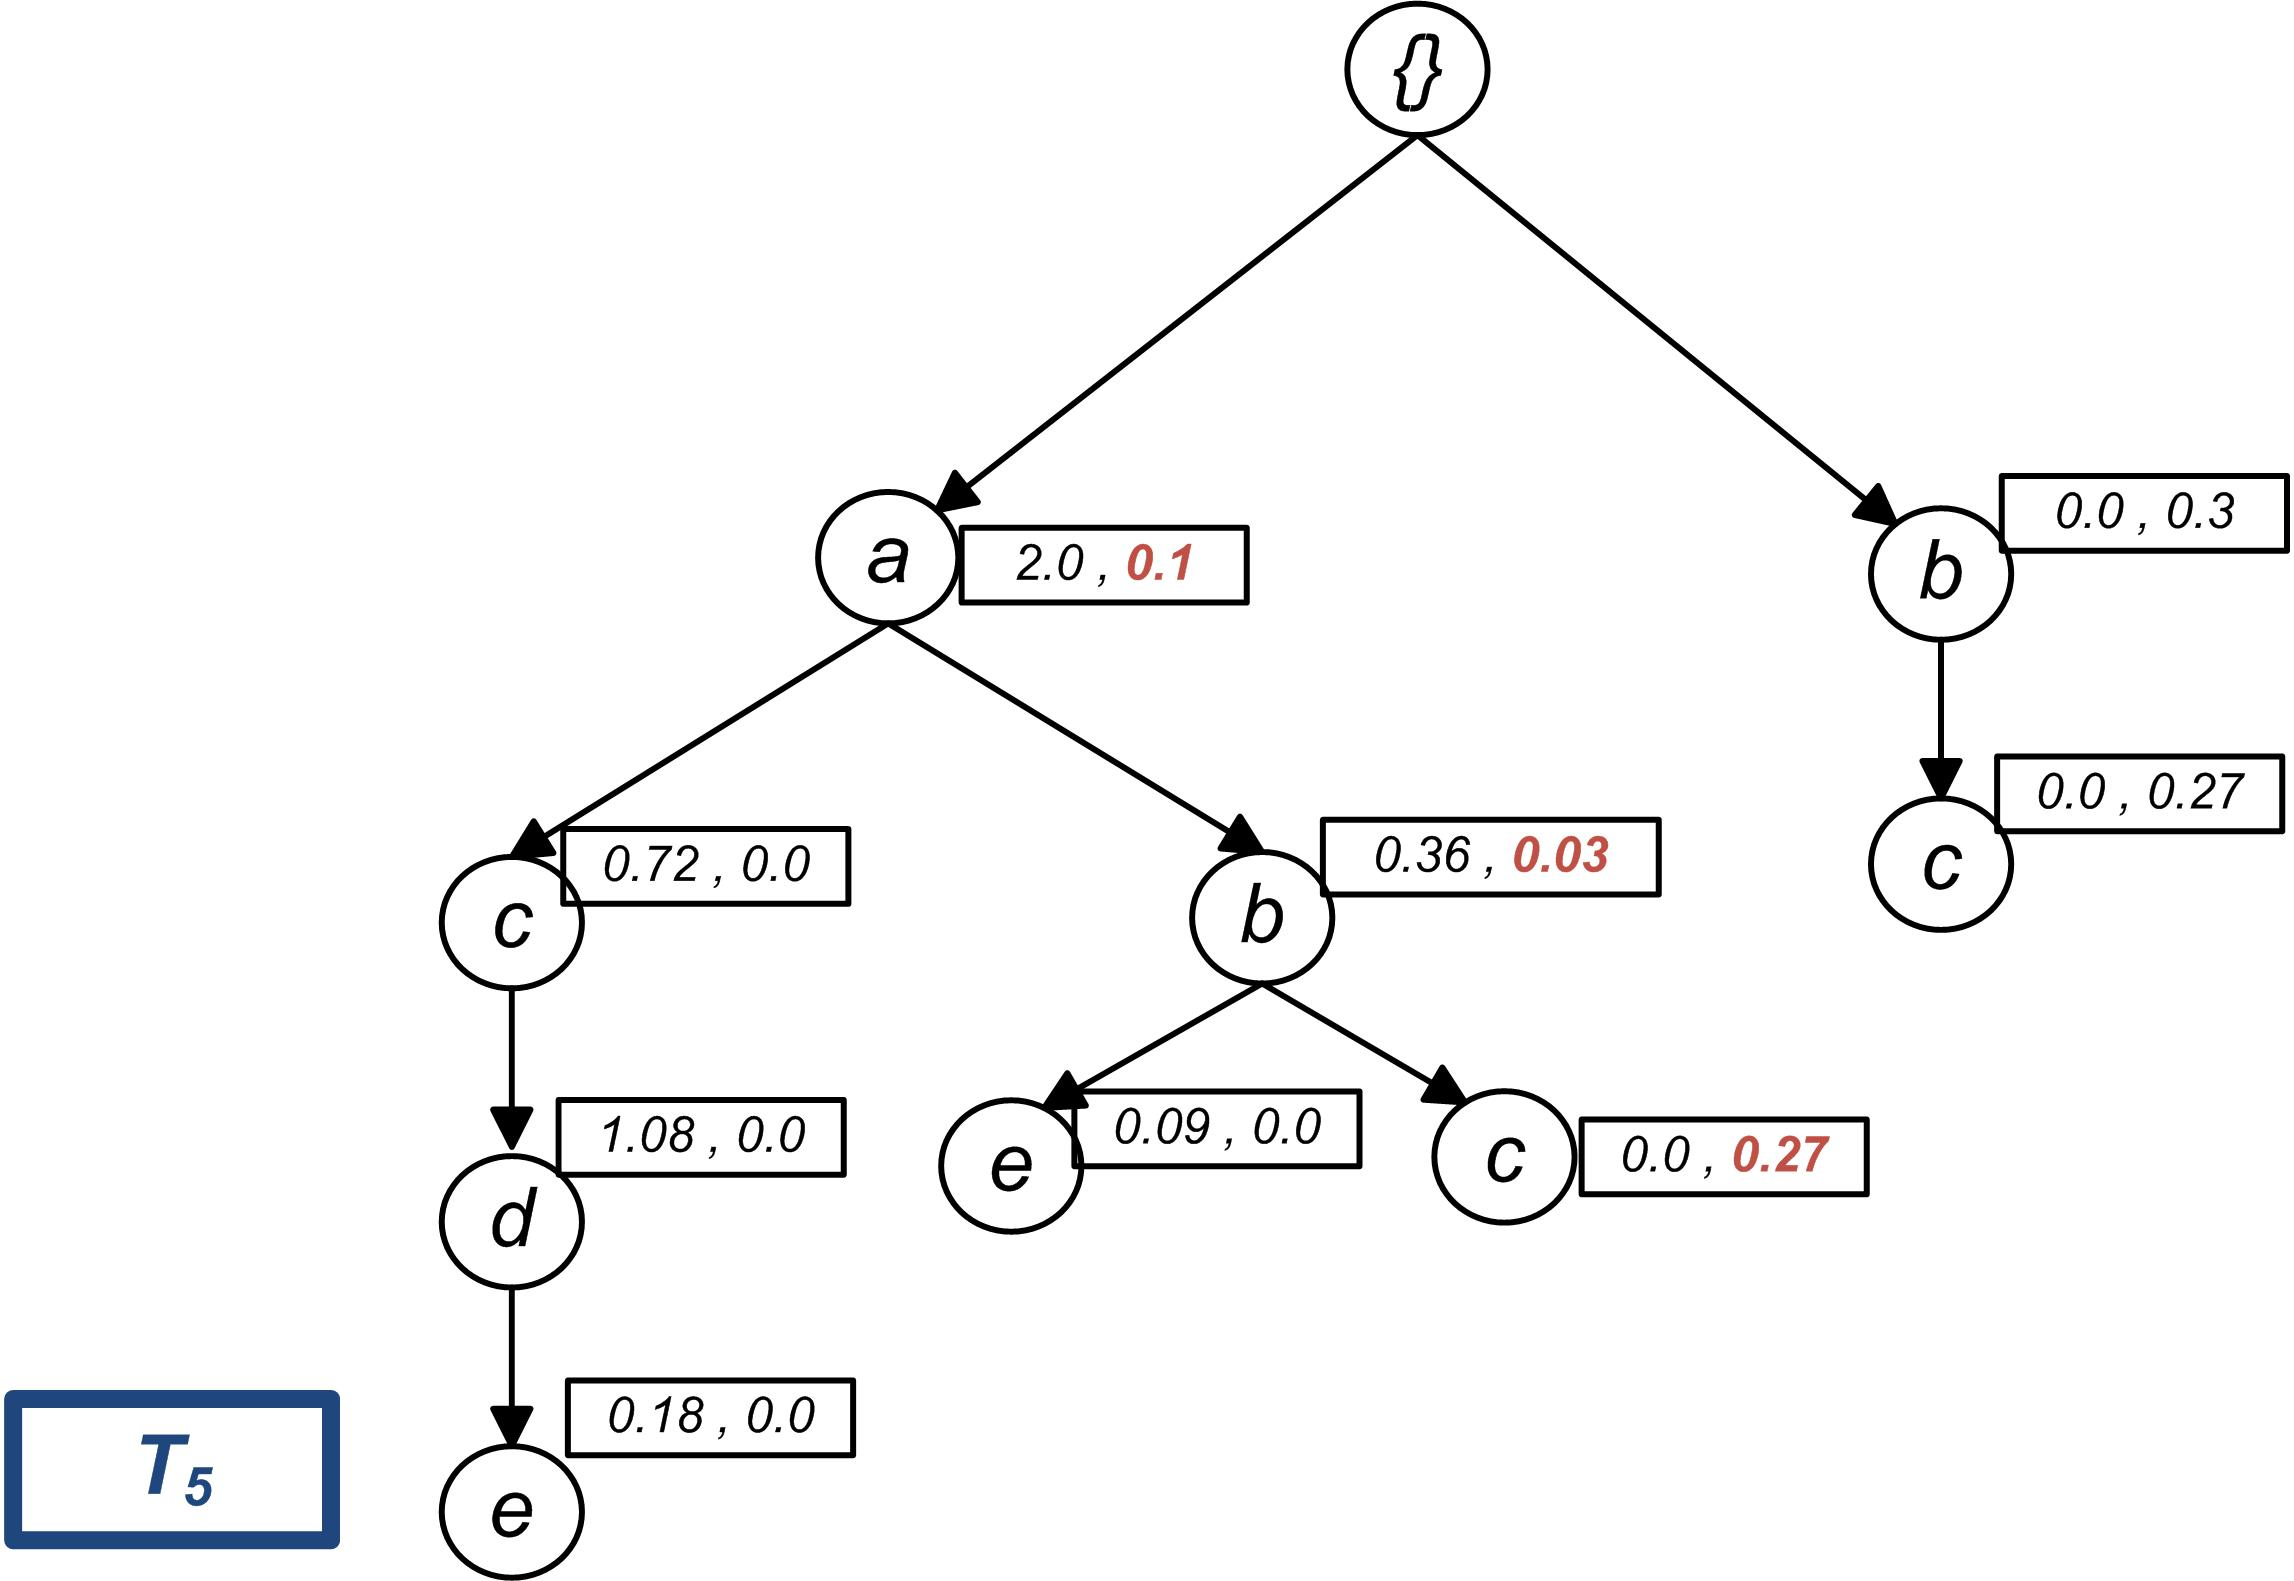
\includegraphics[width=\textwidth,height=4.0cm]{images/sim_05.jpg}
	    \caption{T\textsubscript{5}}
		\end{subfigure}
	  
	 	\begin{subfigure}[b]{0.31\textwidth}
	 	\centering
	    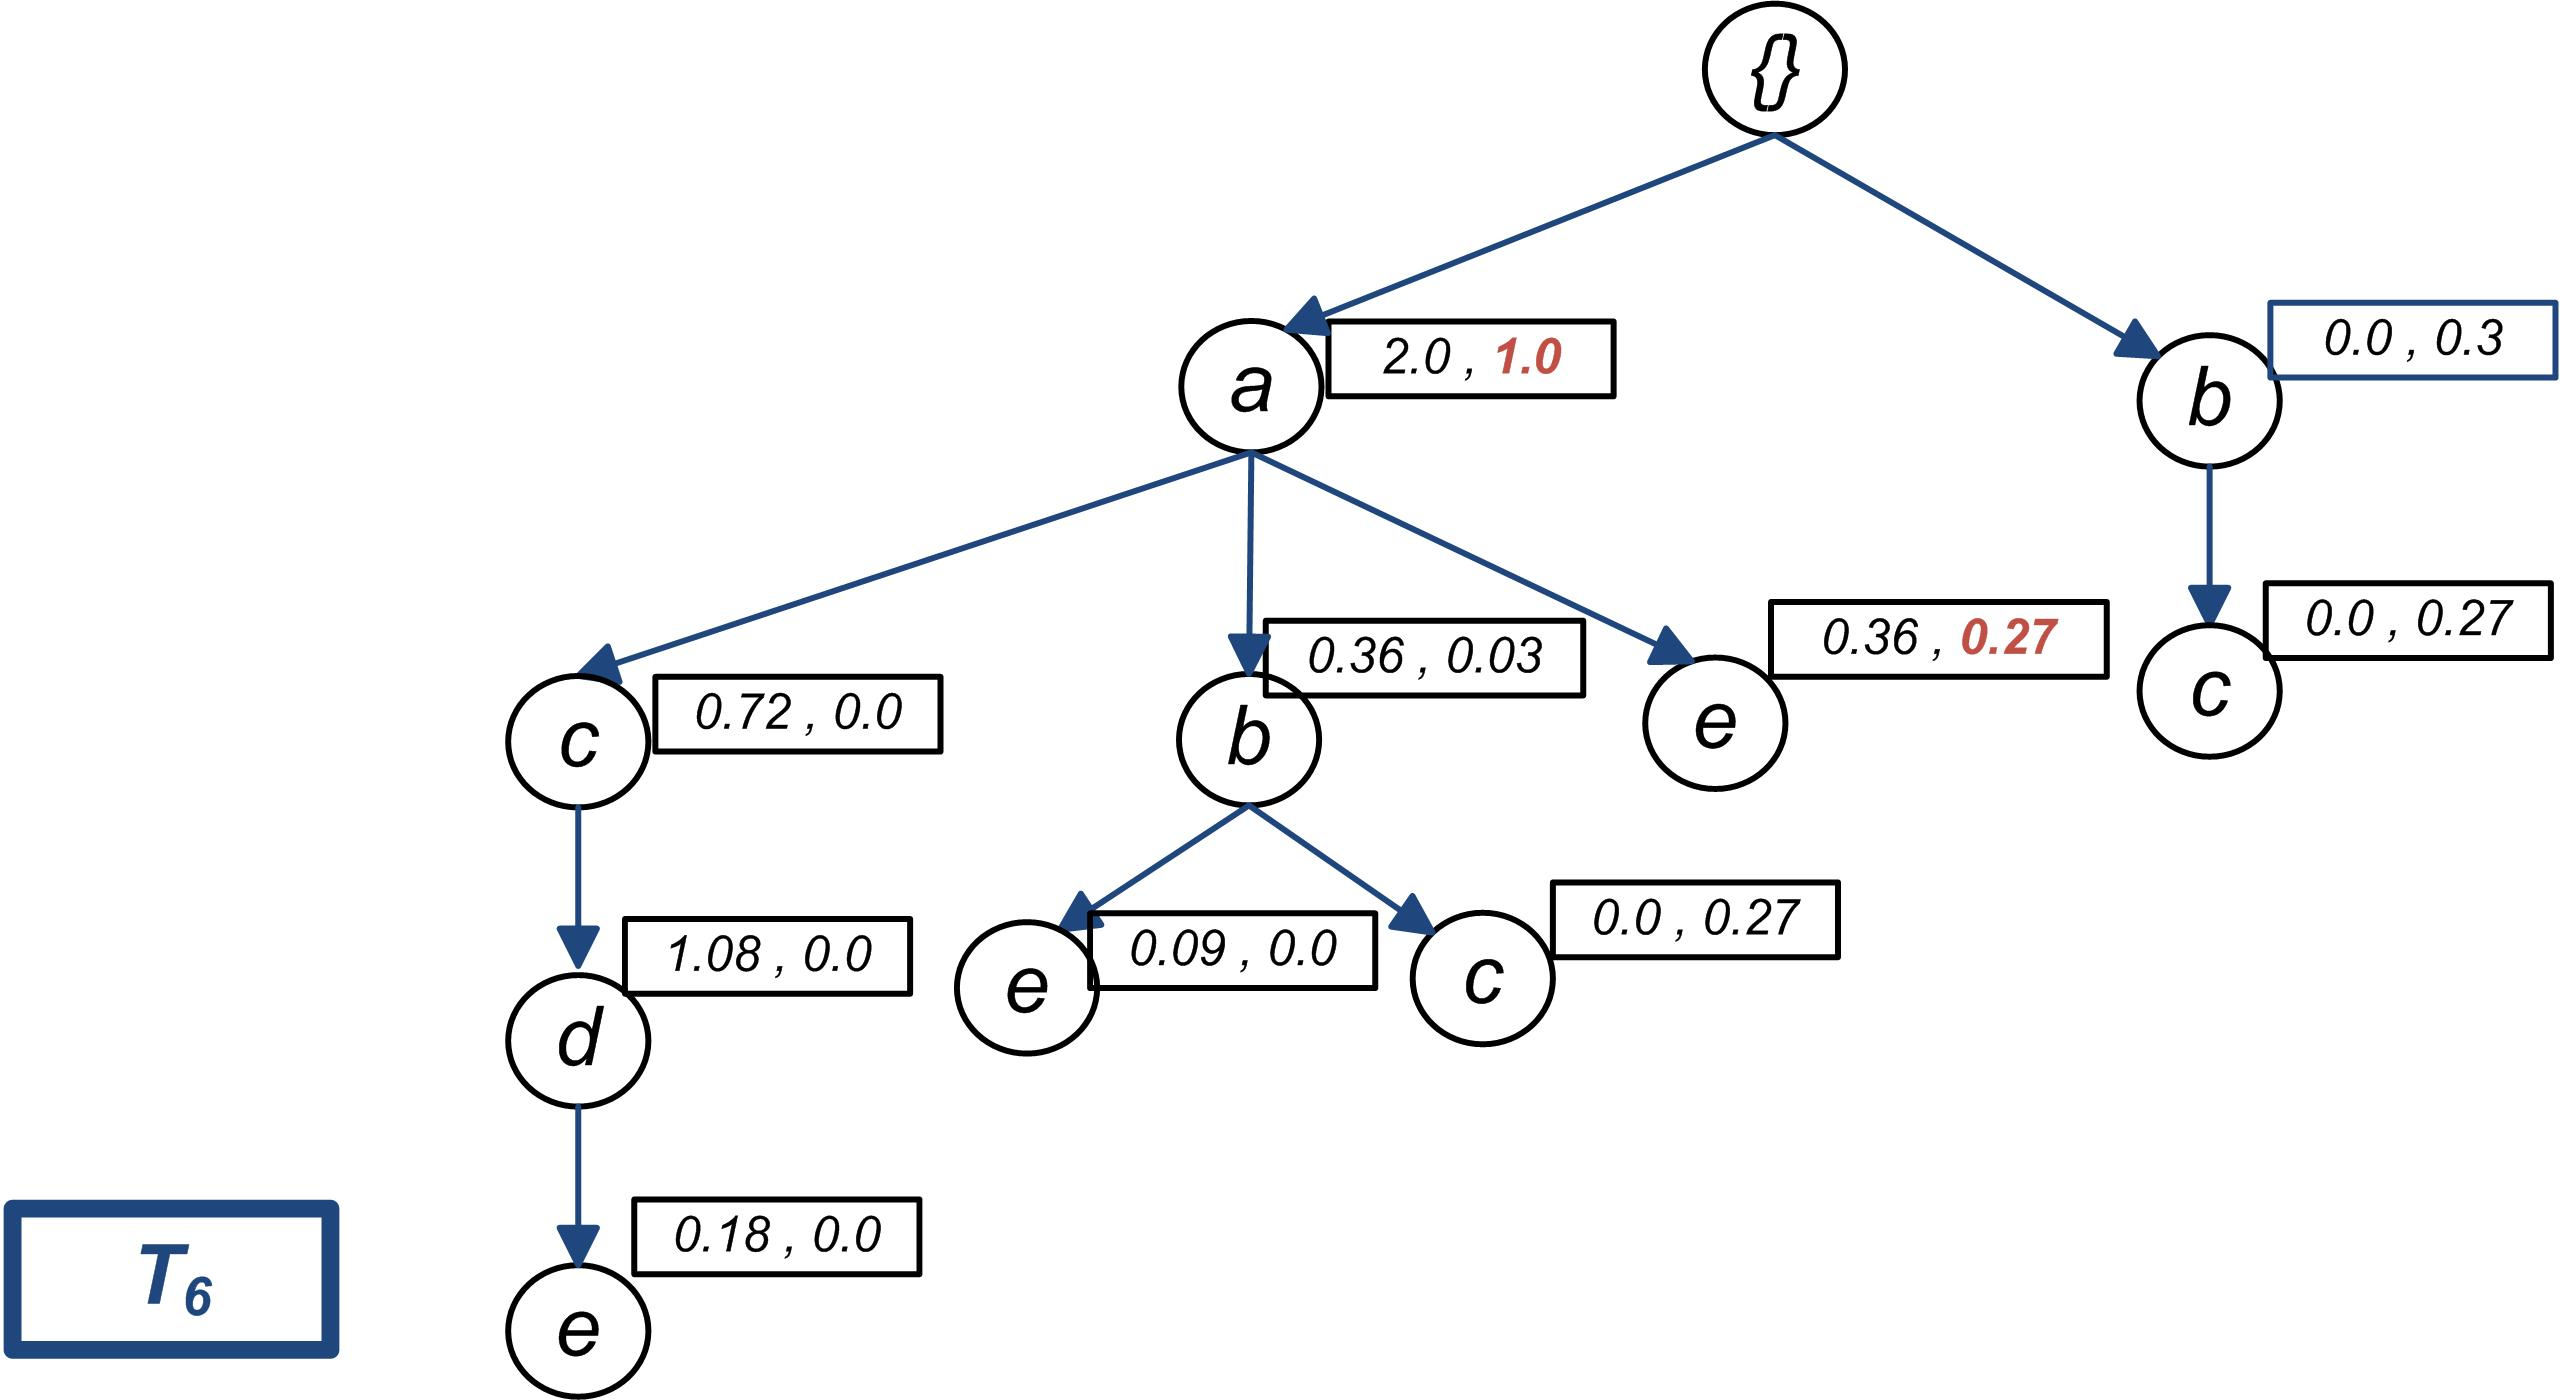
\includegraphics[width=\textwidth,height=3.0cm]{images/sim_06.jpg}
	    \caption{T\textsubscript{6}}
		\end{subfigure}
	}
 \caption{Inserting \emph{T\textsubscript{4}},\emph{T\textsubscript{5}} and \emph{T\textsubscript{6}} in \emph{US-tree}}
 \label{figure:t456}
\end{figure}
\end{frame}
%\end{document}
    Let construct tree for Table-\ref{table:prefix_assigned}. First we insert \emph{Batch-1 (T\textsubscript{1}, T\textsubscript{2}, T\textsubscript{3})} in the window 1. First when inserting the \emph{T\textsubscript{1} - a(0.9), c(0.54), d(0.45), e(0.18)} we insert item \emph{a(0.9)} as a child of root \emph{\{\}} (Figure-\ref{figure:t1}). Update a's prefix value as $0.9$. Then we add \emph{c(0.54)} as a's child update c's prefix value as $0.54$. Aad \emph{d(0.45)} as c's child update d's prefix value as $0.45$. Add \emph{e(0.18)} as d's child update e's prefix value as $0.18$. Thus \emph{T1} is inserted into the tree (Figure-\ref{figure:t1}). For \emph{T\textsubscript{2} - a(0.9), b(0.36), e(0.09)} first we insert \emph{a(0.9)}. Here we found \emph{a} is already inserted so we just update existing node a's prefix value $0.9 + 0.9 = 1.8$ (Figure-\ref{figure:t23}). Then we insert \emph{b(0.36)}. As \emph{a} has no child \emph{b} we insert a new child b and update its prefix value $0.36$. Then insert new e(0.09) as the child of \emph{b}. For \emph{T\textsubscript{3} - a(0.2), c(0.18), d(0.63)} we follow the existing path \emph{a(1.8), c(0.54), d(0.45)} and update corresponding prefix value as $1.8 + 0.2 = 2.0$, $0.54 + 0.18 = 0.72$ and $0.45 + 0.63 = 1.08$ (Figure-\ref{figure:t23}). After inserting the This \emph{T\textsubscript{3}} window 1 is completed. Then we will go for inserting next batch \emph{Batch-2 (T\textsubscript{4}, T\textsubscript{5}, T\textsubscript{6})} in the tree. For \emph{Batch-2} we shall put prefix value in the window's newest place. And thus the latest batch becomes the most recent information. For inserting \emph{T\textsubscript{4} - b(0.3), c(0.27)} we insert new node \emph{b} as there is no child b of root node \emph{\{\}}. So we insert \emph{b} as a child of root \emph{\{\}}. Update its prefix value as $0.3$. Then insert \emph{c(0.27)} as child of \emph{b} and update prefix value $0.27$. Here as this \emph{T\textsubscript{4}} is inserting in \emph{Batch-4} we update prefix value for recent batch's information. Next we insert \emph{T\textsubscript{5} - a(0.1), b(0.03), c(0.27)}. We merge \emph{a(0.1), b(0.03)} with previous \emph{a, b } nodes and update prefix value $0.1$ and $0.03$ in the second batch's portion and insert new node \emph{b} as a child of \emph{b} and update its prefix value as $0.27$ (Figure-\ref{figure:t456}).
    %\documentclass{article}
%\usepackage{graphicx}
%\usepackage{caption}
%\usepackage{subcaption}
%
%\begin{document}
\begin{figure}
  \centering
	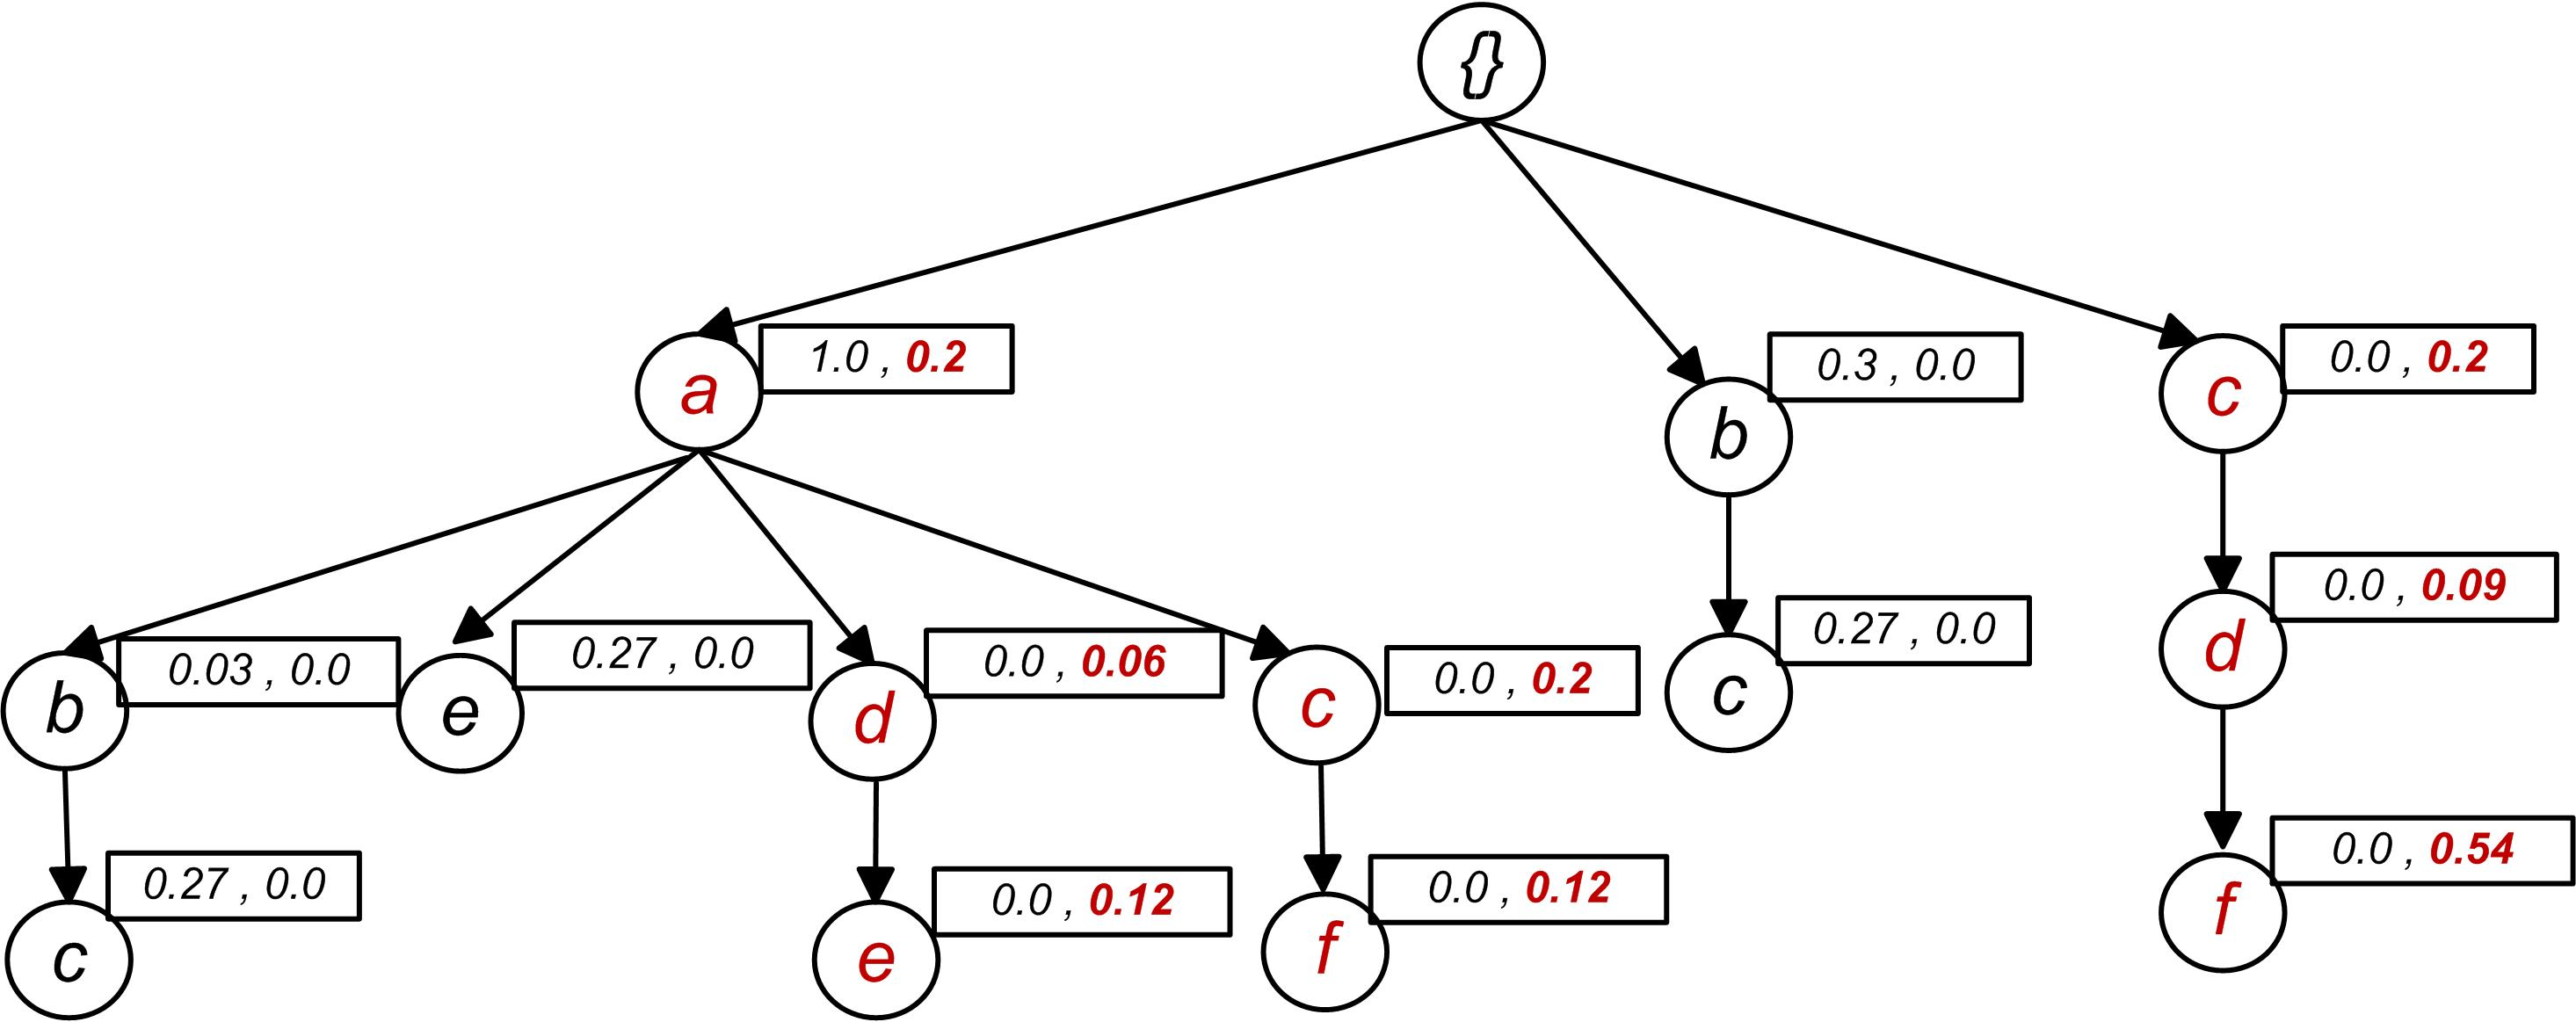
\includegraphics[width=.8\textwidth]{images/sim_789.jpg}  
	\caption{Inserting \emph{T\textsubscript{7}, T\textsubscript{8}, T\textsubscript{9}} into \emph{US-tree} after sliding}
	\label{figure:w2}
\end{figure}
%\end{document}
    Now our window is completed and can our \emph{USFP-growth} mine \emph {US-tree}. When new transaction batch comes like \emph{Batch-3 (T\textsubscript{7}, T\textsubscript{8}, T\textsubscript{9})} comes to be inserted into the tree then first we have to slide the window. For this when we construct the tree we maintain a header table which contains the information for the oldest data. Thus pointer points to the oldest data can be found easily and slide the whole tree. Figure-\ref{figure:slide} shows the sliding and getting the old data removed tree and ready to insert next batch \emph{Batch-3}. After inserting \emph{Batch-3} we get the tree like Figure-\ref{figure:w2}. 
    \documentclass{article}
\usepackage{graphicx}
\usepackage{caption}
\usepackage{subcaption}

\begin{document}

\begin{frame}

\begin{figure}[!tbp]
  \centering
	\fbox{  
	 	\begin{subfigure}[b]{0.44\textwidth}
	 	\centering
	    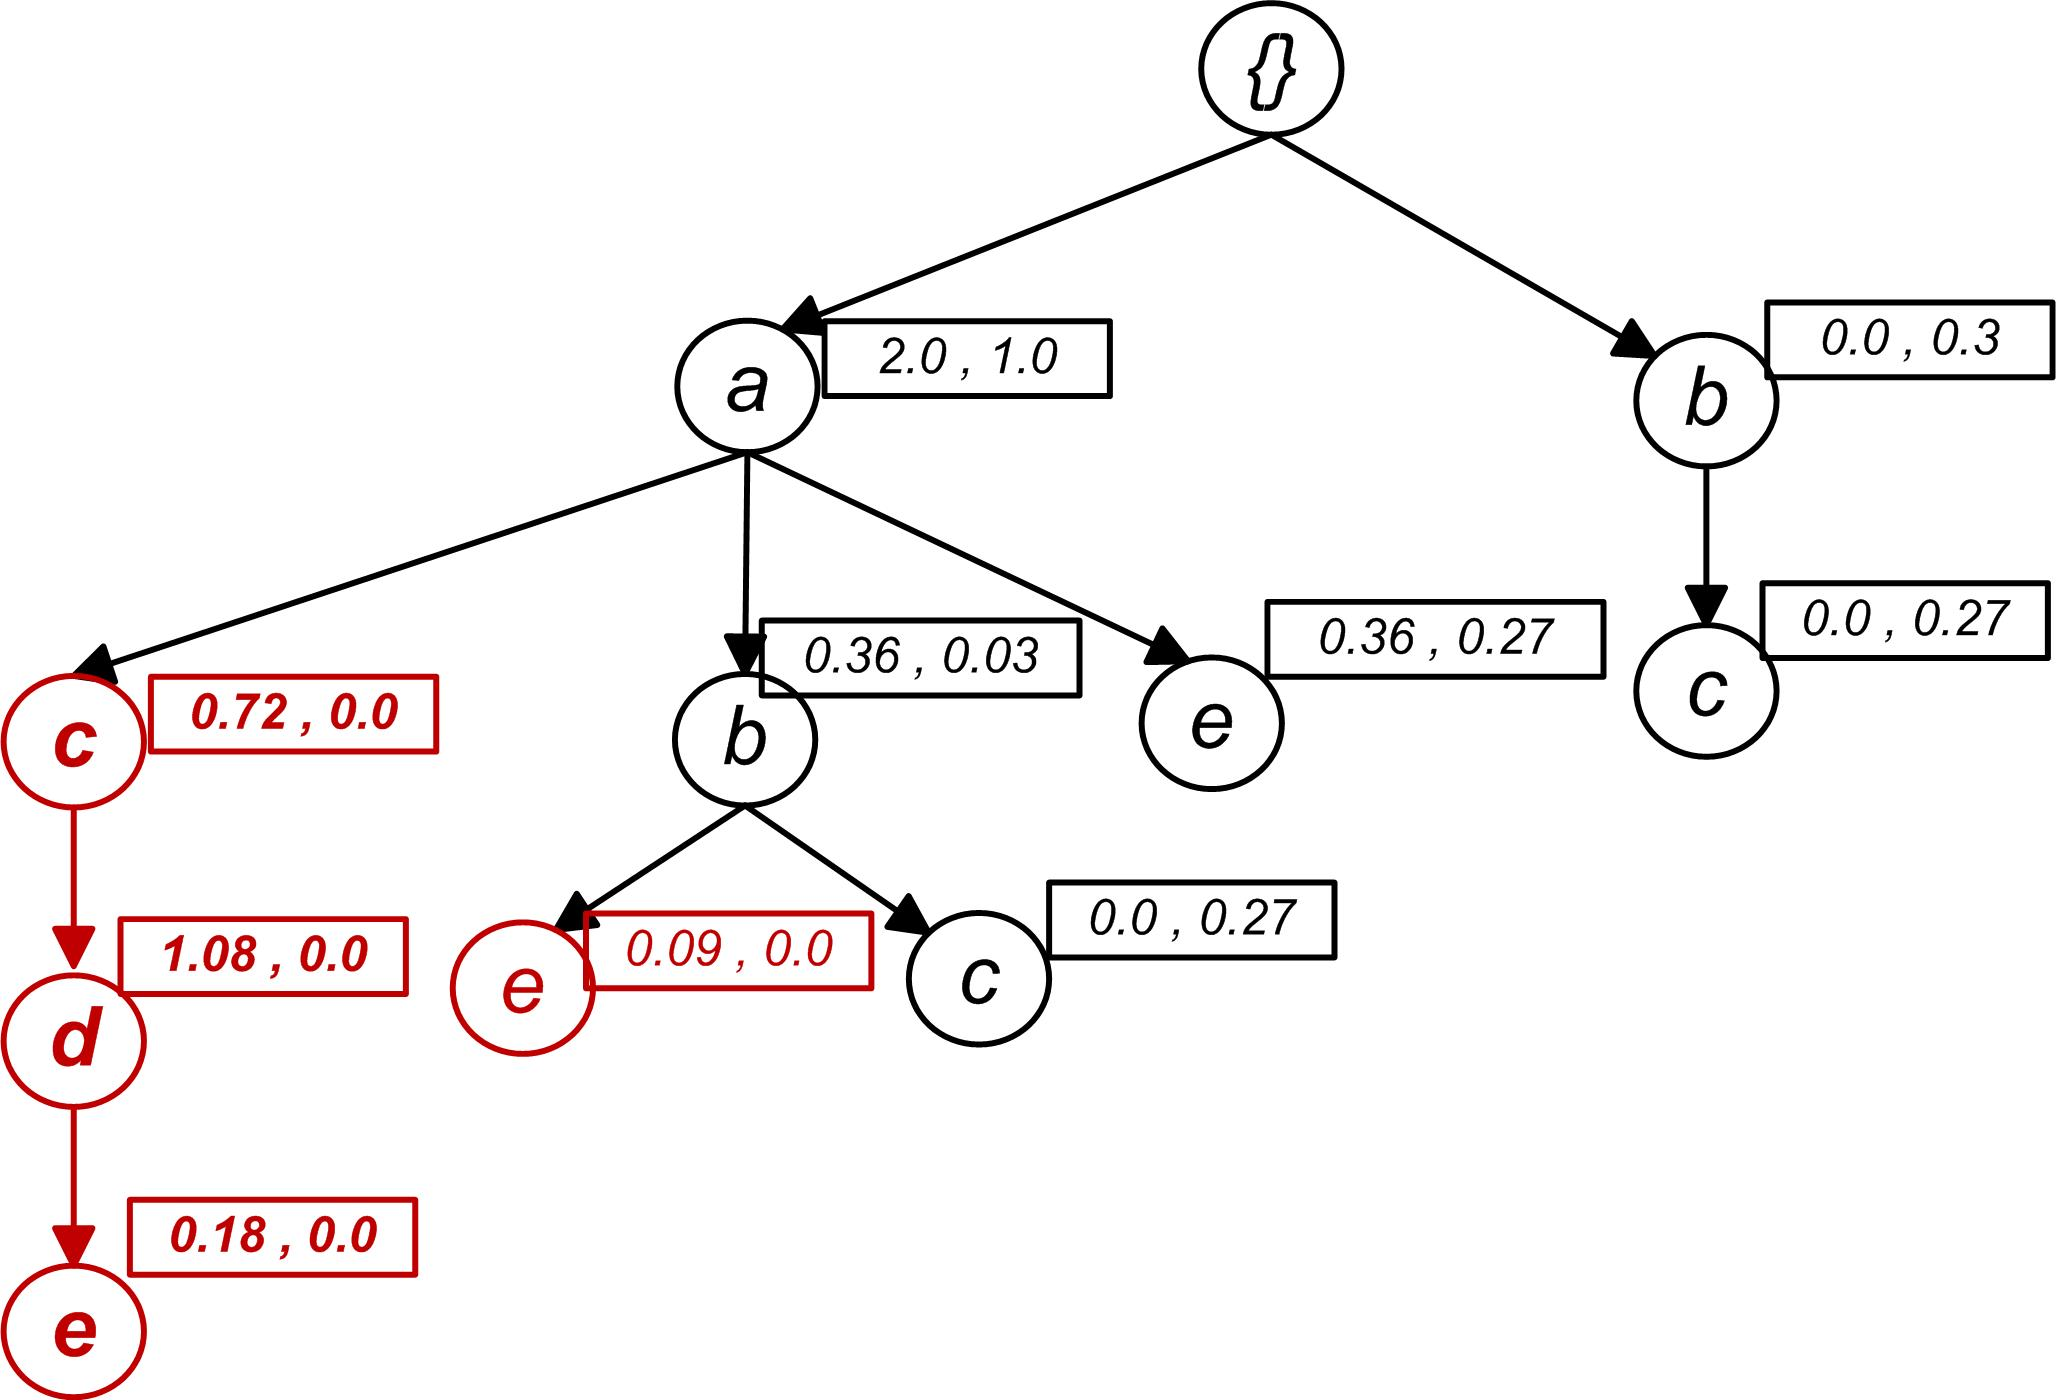
\includegraphics[width=\textwidth,height=4.5cm]{../images/sim_06_slide.jpg}
	    \caption{Before Sliding}
		\end{subfigure}
 
	 	\begin{subfigure}[b]{0.36\textwidth}
	 	\centering
	    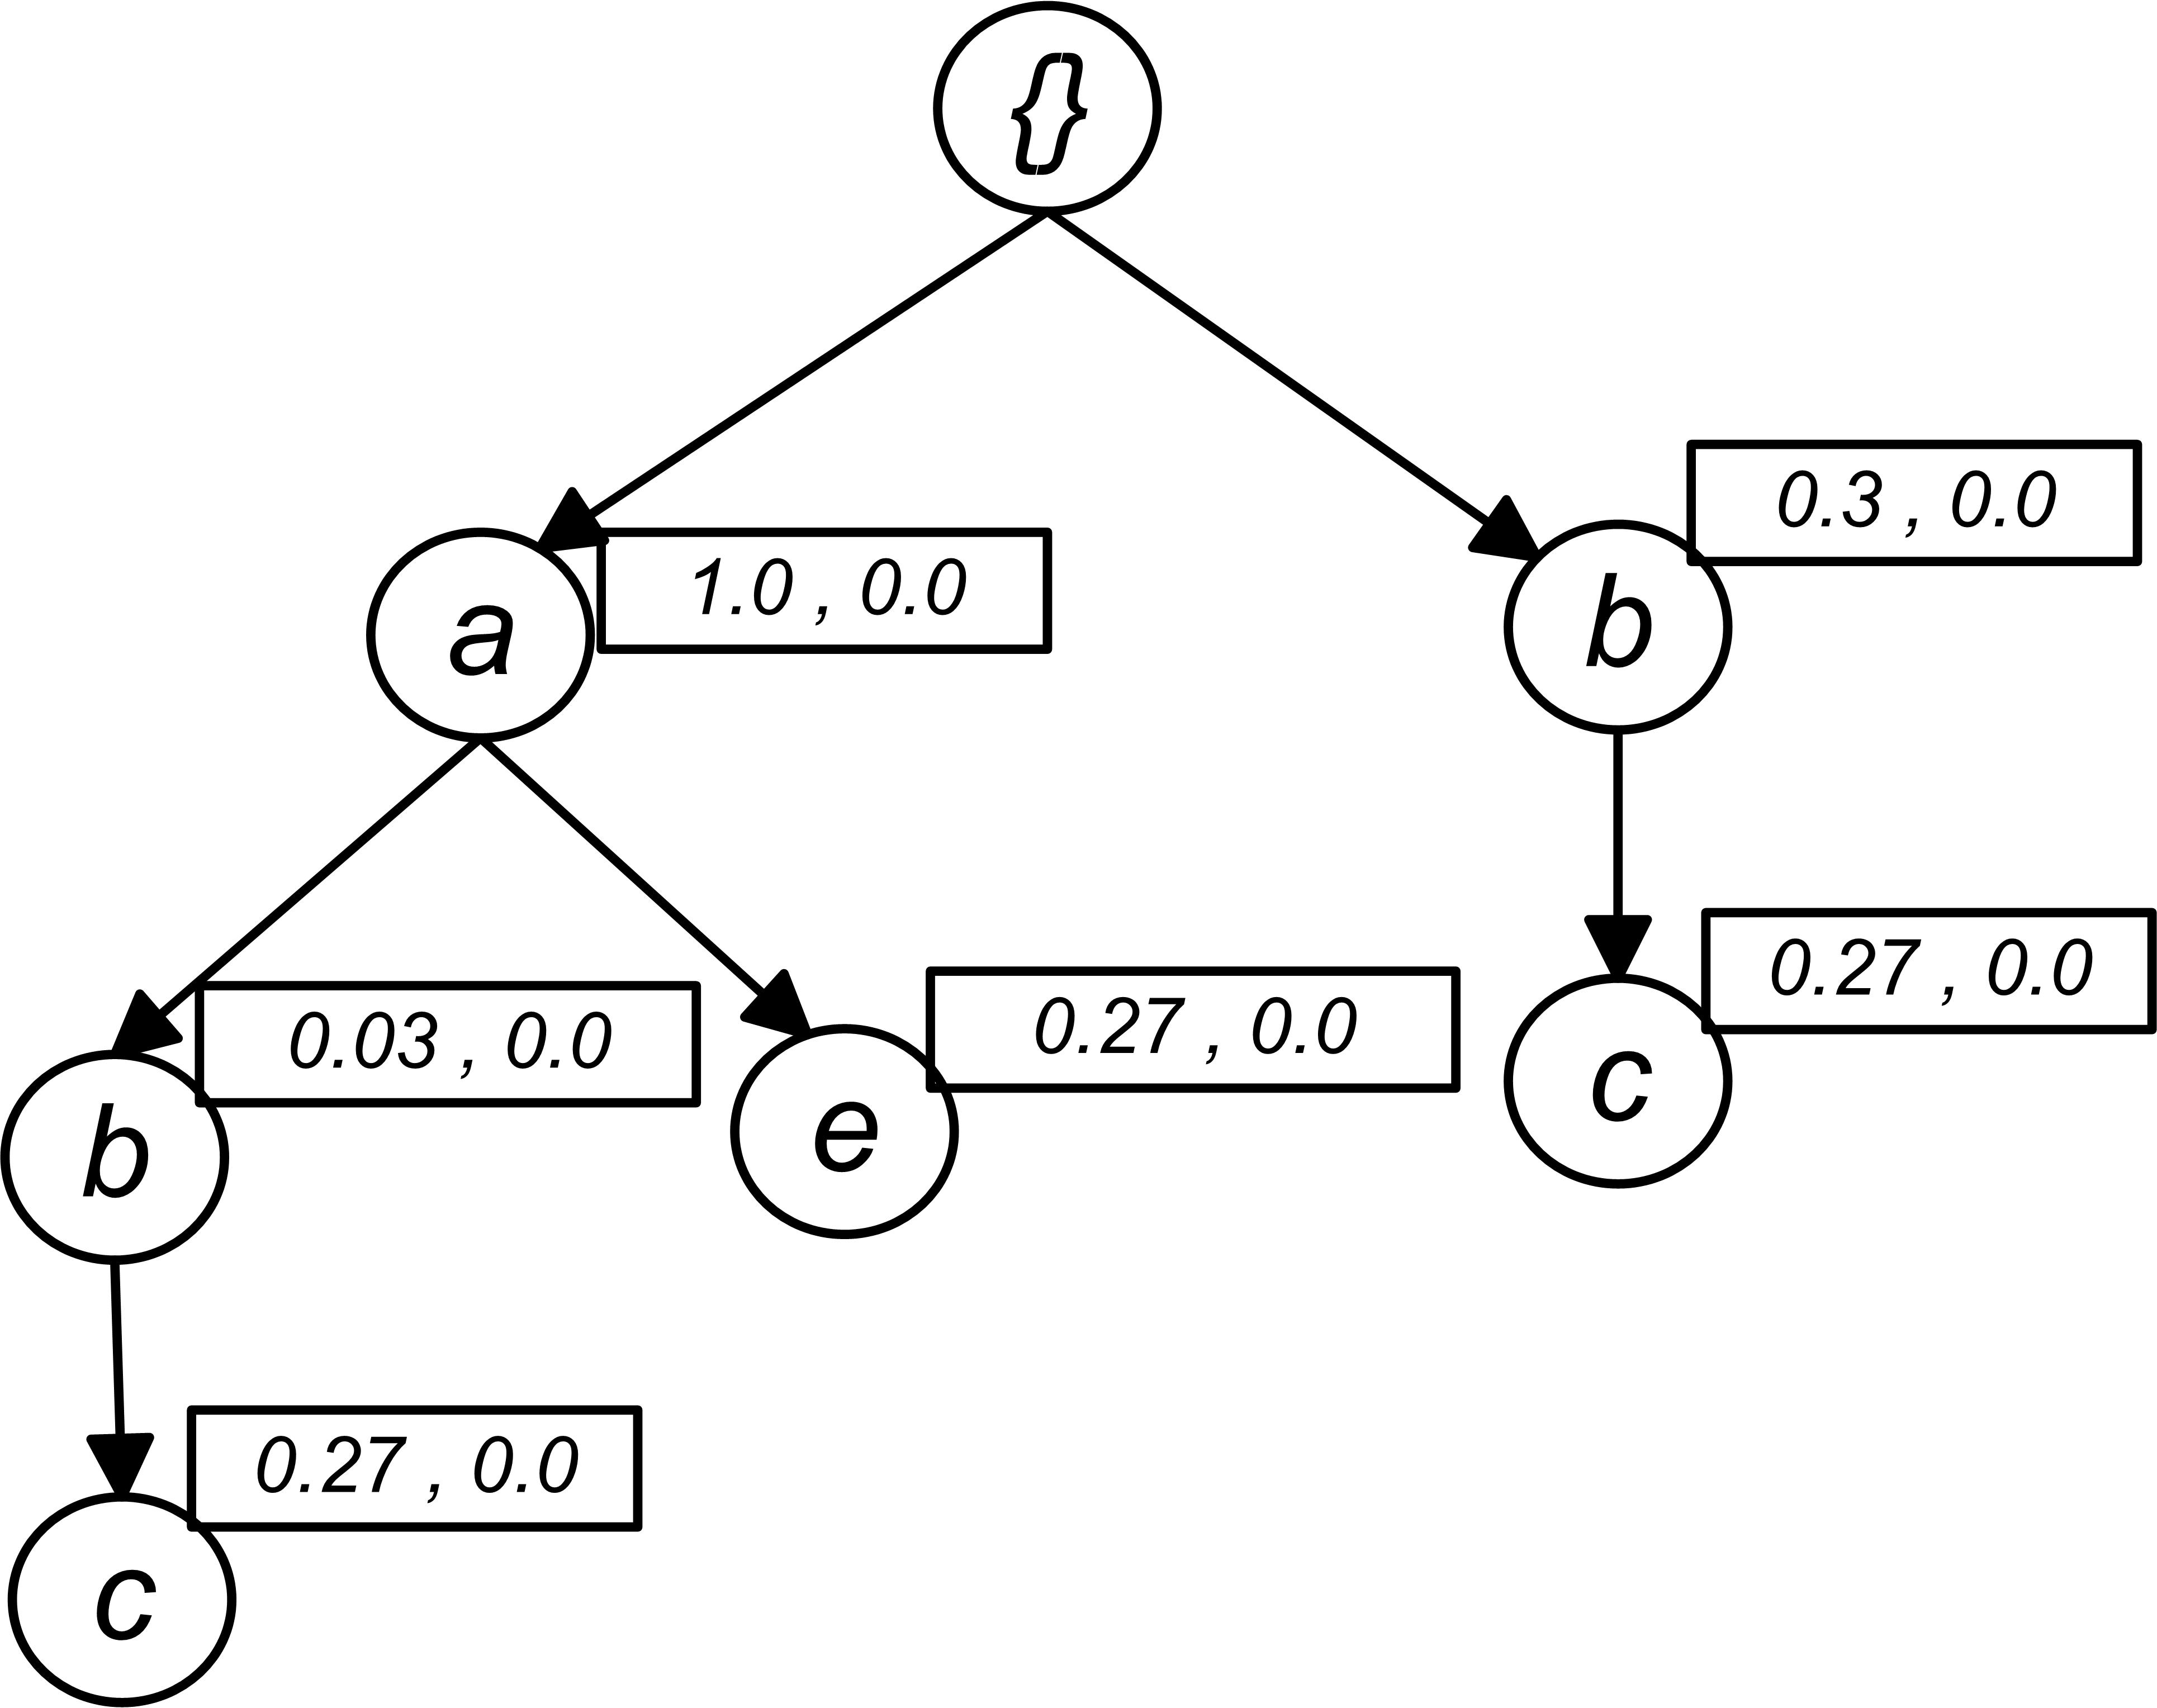
\includegraphics[width=\textwidth,height=4.5cm]{../images/sim_06_slide_2.jpg}
	    \caption{After Sliding}
		\end{subfigure}
	}
 \caption{Sliding \emph{US-tree}}
\end{figure}
\end{frame}



\end{document}
    In the described \emph{US-tree} construction process we see that tree sharing is very much common and regular. That makes our tree very compact and memory needed to hold items becomes less. Moreover, the tree construction time improves surprisingly. When to mine this \emph{US-tree} we can gain a lot time when mining. As the tree size is small, conditional tree will be much more less when mining. We will gain a lot time when trying to mine the conditional trees. In the experimental result section we will provide necessary graphs for our simulations.
    \subsection{Mining US-tree FPUS-growth}
    In this section we will discuss about our mining algorithm \emph{USFP-growth} (algorithm-\ref{algorithm:mine}) That will find frequent patterns. For mining we used \emph{FP-growth} like approach. Generally, we can remove all the nodes having support less than \emph{minimum support}. From header table we get such information that which nodes is less than \emph{minimum support}. We told earlier that for \emph{U\textsuperscript{cap}} value we took the upper limit, we also can we can remove all the nodes having prefix value less than \emph{minimum support}. In this process we can eliminate most of the infrequent nodes from tree. For this purpose we used header table that was created when creating the \emph{US-tree}. Then we construct conditional tree starting from the lowest support holding node. From header table we also get the position of all nodes containing same item in the tree. 
    Let’s mine the tree we constructed earlier. Figure-\ref{figure:min_before} is \emph{US-Tree} for mining and corresponding header table before starting mining. From the header table, we get that support of \emph{a} is $3.00$, \emph{b} is $1.00$, \emph{c} is $3.30$, \emph{d} is $1.20$, \emph{e} is $0.60$. So, \emph{e} is not frequent for one item set frequent pattern. So it is sure that no item set contains \emph{e} will be frequent. That is the basic upward closure property of frequent item set. So we remove all the nodes of \emph{e} and get the new mining tree Figure-\ref{figure:min_ready} and its header table. Here we find all one item sets that are frequent and that is \emph{\{a\}, \{b\}, \{c\} \{d\}} Now we will construct conditional tree for the found frequent one item and mine the conditional tree. But items having total \emph{U\textsuperscript{cap}} less than \emph{minimum support} is not needed to construct conditional tree because this \emph{U\textsuperscript{cap}} value has been take as the upper bound. So total \emph{U\textsuperscript{cap}} value less than \emph{minimum support} indicates that item must not be exists in the $2$ or more frequent item set. So we do not construct conditional tree for these items.
    We construct conditional tree from items having lowest total \emph{U\textsuperscript{cap}} value greater than \emph{minimum support}. As \emph{b} having total \emph{U\textsuperscript{cap}} is $.69$ \emph{b}, is ignored for constructing conditional tree. Then the next candidate is \emph{d}. From header table pointer we find that there is only one path item \emph{d} exists in the mining tree Figure-\ref{figure:min_ready}. That is \{\emph{a, c, d}\}:$1.08$. So we create conditional tree and update all nodes mining probability with \emph{d's} \emph{U\textsuperscript{cap}} $1.08$. For this conditional tree Figure-\ref{figure:d_cond} the header tables says all the nodes in the tree are having \emph{U\textsuperscript{cap}} greater than \emph{minimum support} $.9$. So, all the items are ready to be constructed as conditional tree. As here is only one branch so we do not further construct conditional tree and take all the combinations as frequent items Figure-\ref{figure:d_cond} Table. So we find \emph{\{dc\}, \{da\}, \{dca\}} as frequent pattern. Next we create conditional tree for \emph{c}. Here c exists in the tree for three path those are \emph{\{a, c\} : $0.72$ , \{a , b, c\} : $.027$ and \{b, c\} : $0.27$}. So we create conditional tree (Figure-\ref{figure:c_cond}). Total mining value of \emph{c} is the sum of item caps in each respective path of \emph{c}. From the header we see that \emph{b} has total cap having less than \emph{minimum support} so we remove \emph{b} and create two item set \emph{\{ca\}}. Next we construct \emph{ca} conditional tree that contains only root (\emph{\{\}}). So no further tree is needed to be constructed and minned. Than we create conditional tree for \emph{a}. And find only root \emph{\{\}}. Thus we get all the frequent patterns. All the patterns are \emph{\{a\}, \{b\}, \{c\} \{d\}, \{dc\}, \{da\}, \{dca\} and \{ca\}}. As we have found all patterns from upper bound, so that it is guaranteed that there will be no false negative. But some false positive can be exists in the found frequent item set as there may be some value less than max value we assumed. So in the next section we will show an approach that eliminates the all false positives (if exists) in the data set.
    %\documentclass{article}
%\usepackage{caption}
%\usepackage{graphicx}
%\begin{document}

\begin{figure}
\begin{minipage}{0.40\textwidth}
  \centering
  
	\begin{center}
	\begin{tabular}{ |c|c|c| } 
 	\hline
 		Item&\emph{U\textsuperscript{cap}}&Support\\ \hline\hline
 		a &  3.00  & 3.00	\\ \hline
 		c &  1.26  & 3.30	\\ \hline
 		d &  1.08  & 1.20	\\ \hline
 		e &  0.54  & 0.60	\\ \hline
 		b &  0.69  & 1.00	\\ \hline
\end{tabular}
\end{center}   
  \captionof{table}{Header Table of US-tree}
\end{minipage}
\hfill
\begin{minipage}{0.40\textwidth}
  \centering
  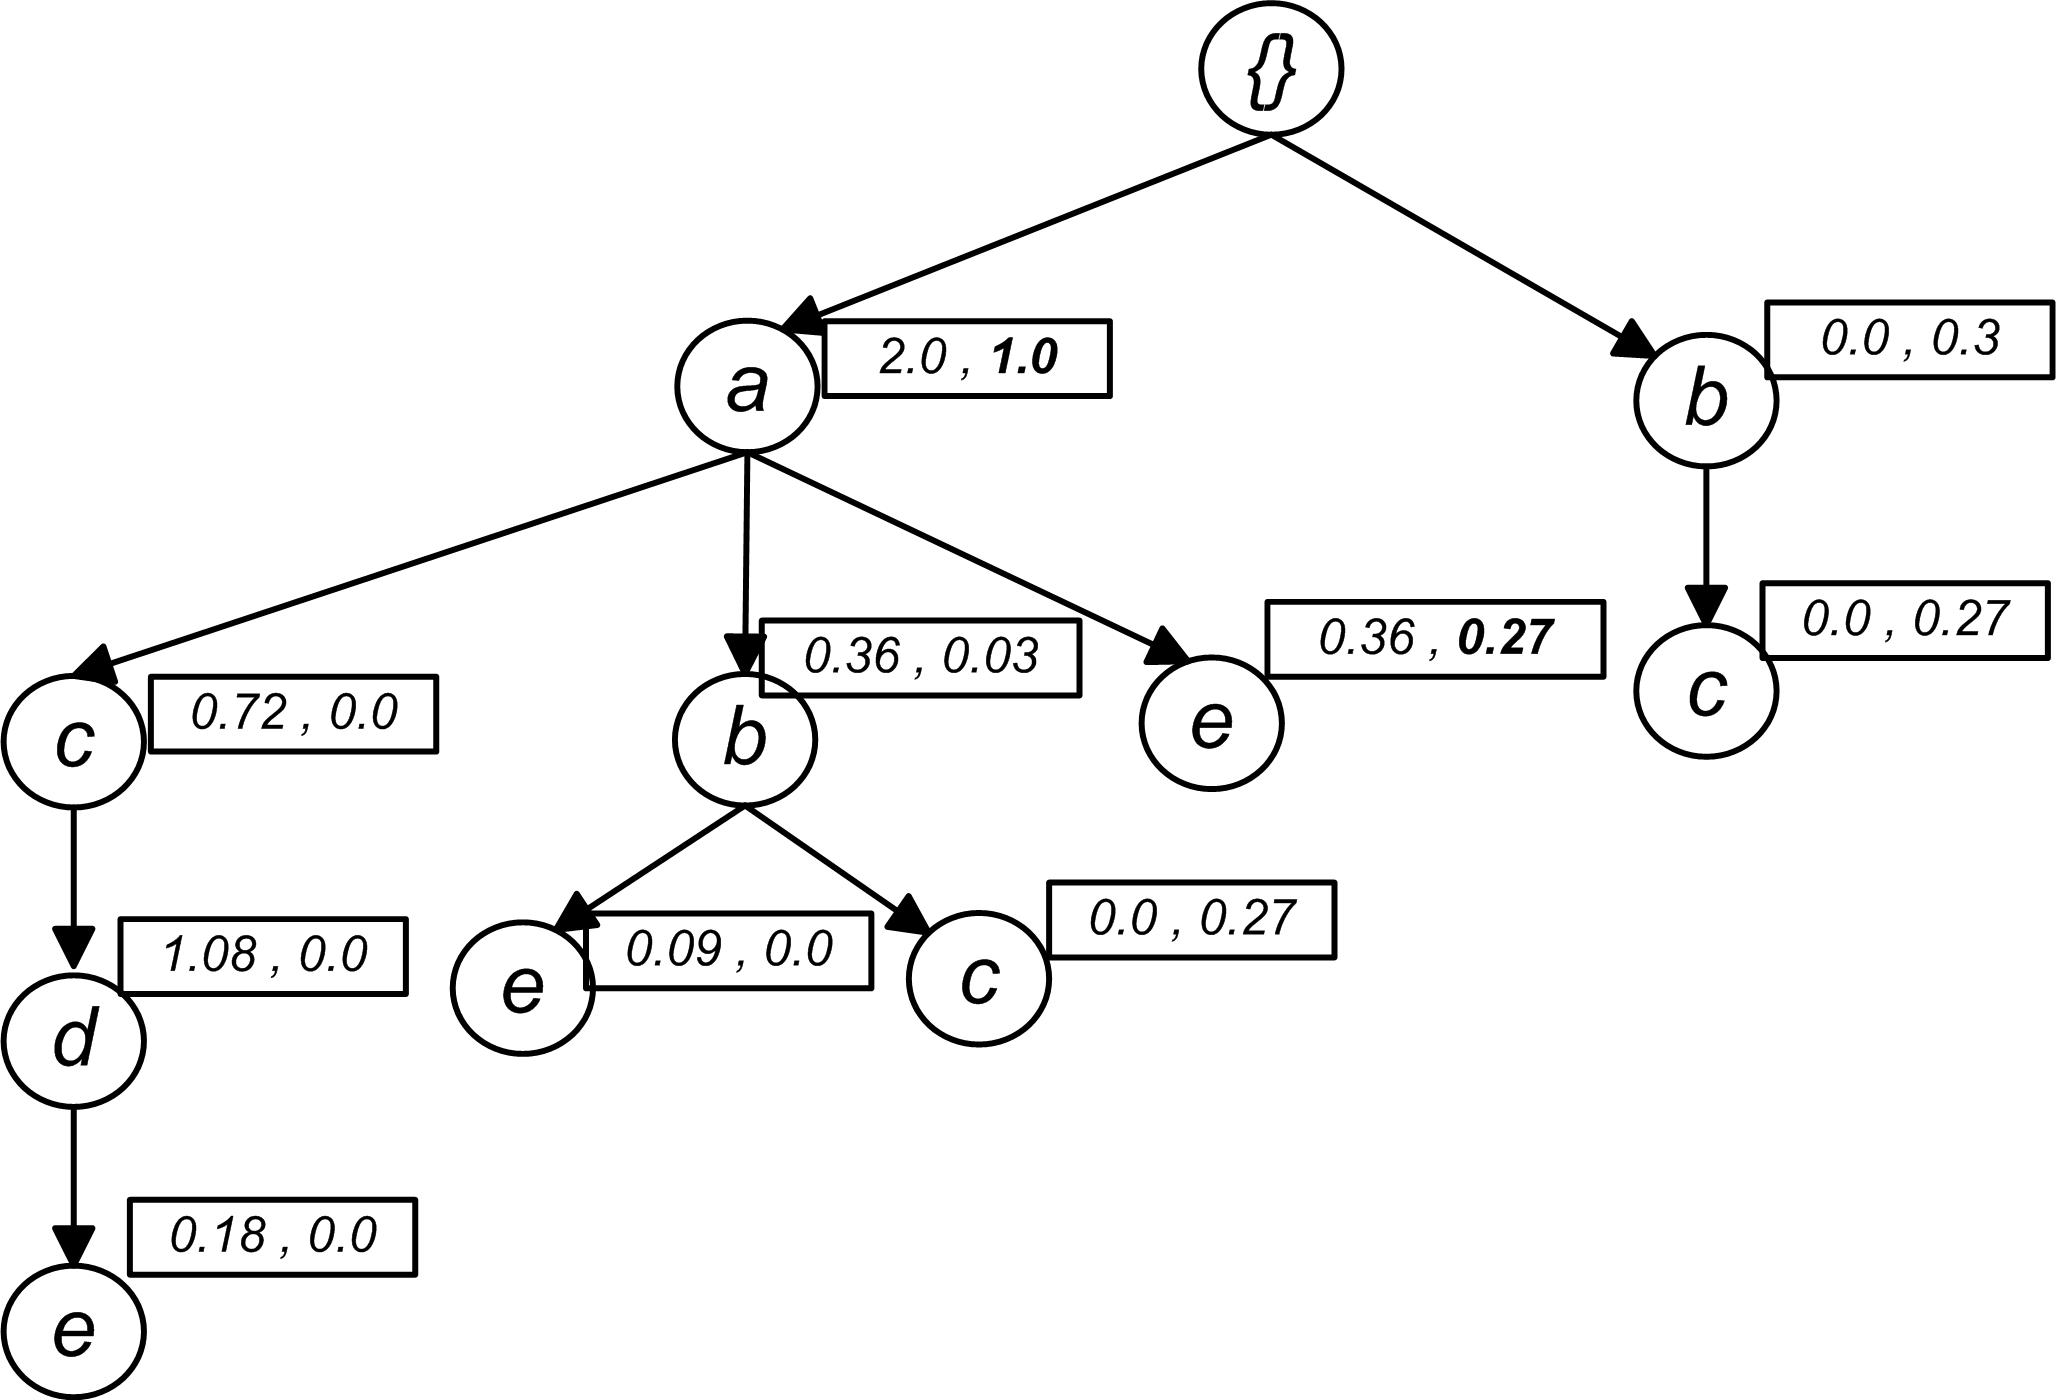
\includegraphics[width=\textwidth]{images/us_tree.jpg}
  \captionof{figure}{US-tree}
\end{minipage}
\caption{US-tree and Header Table}
\label{figure:min_before}
\end{figure}


\begin{figure}
\begin{minipage}{0.40\textwidth}
  \centering
  
	\begin{center}
	\begin{tabular}{ |c|c|c| } 
 	\hline
 		Item&\emph{U\textsuperscript{cap}}&Support\\ \hline\hline
 		a &  3.00  & 3.00\\ \hline
 		c &  1.26  & 3.30\\ \hline
 		d &  1.08  & 1.20\\ \hline
 		b &  0.69  & 1.00\\ \hline
\end{tabular}
\end{center}  
  
  
  \captionof{table}{Header Table for Mining}
\end{minipage}
\hfill
\begin{minipage}{0.40\textwidth}
  \centering
  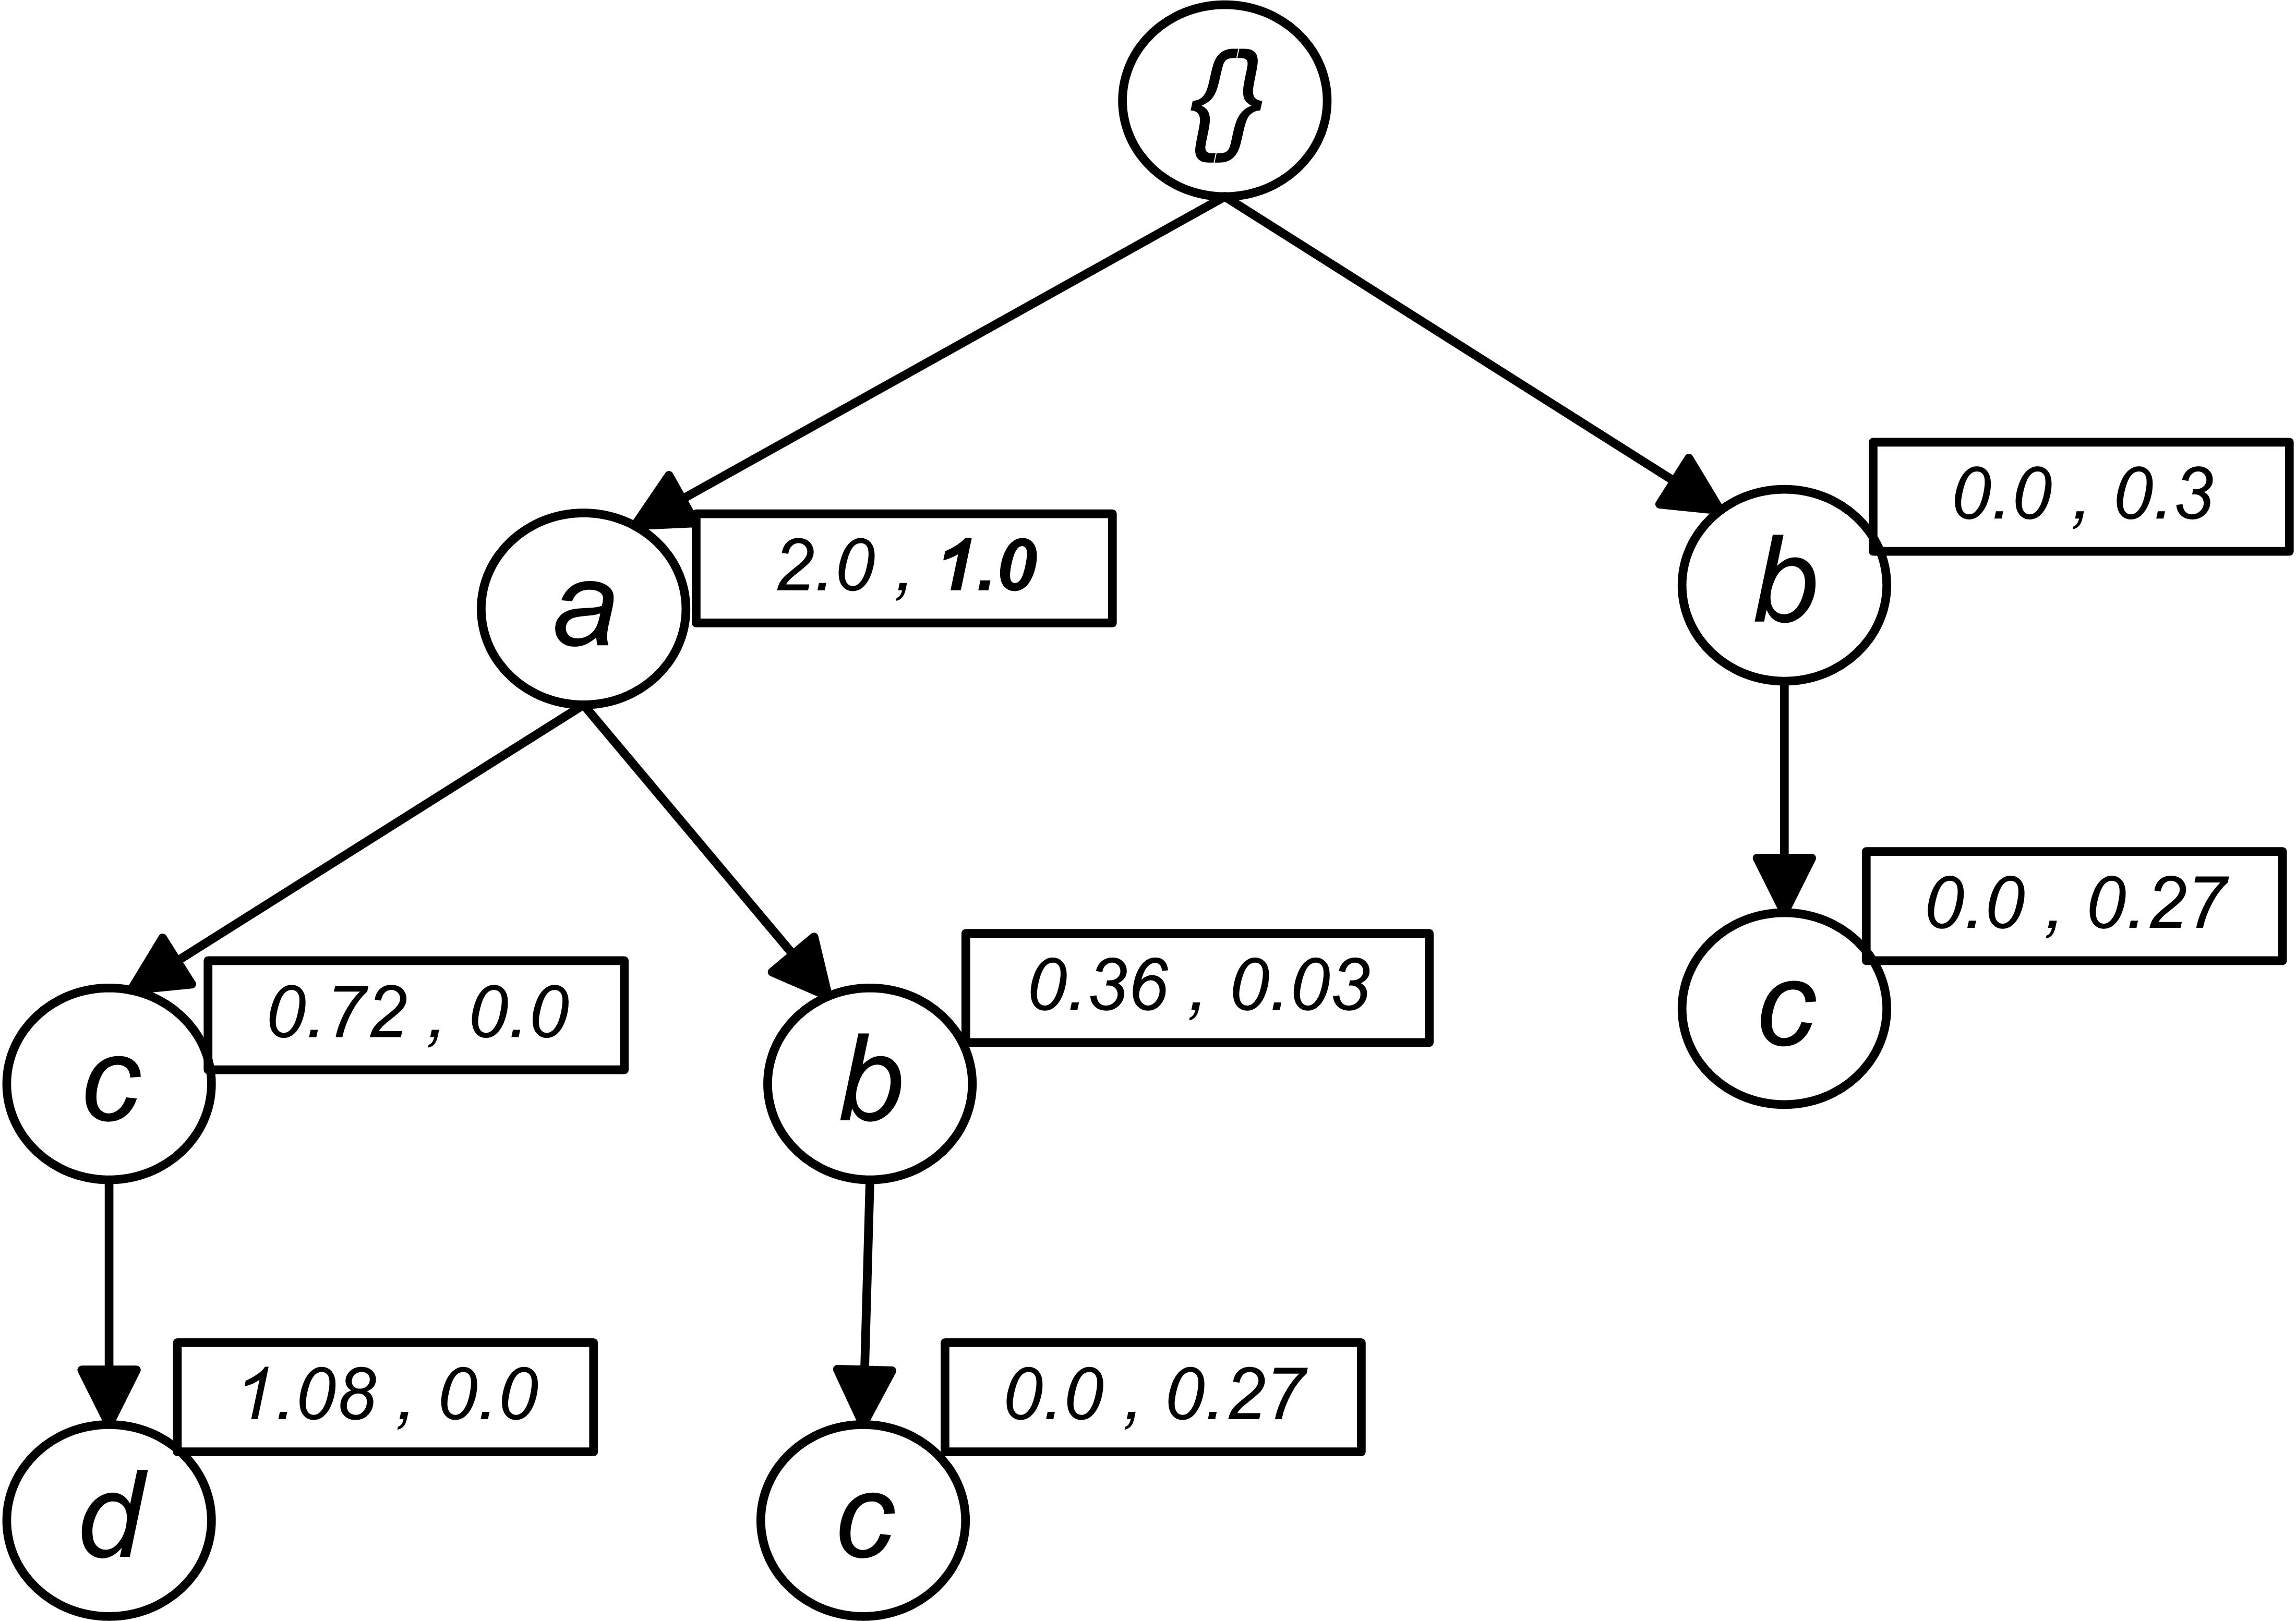
\includegraphics[width=\textwidth]{images/M_TREE.jpg}
  \captionof{figure}{US-tree for Mining}
\end{minipage}
\caption{US-tree and Header Table for Mining}
\label{figure:min_ready}
\end{figure}
%\end{document}
    %\documentclass{article}
%\usepackage{caption}
%\usepackage{graphicx}
%\begin{document}
\begin{figure}
\begin{minipage}{0.40\textwidth}
  \centering
	\begin{center}
	\begin{tabular}{ |c|c| } 
 	\hline
 		Item&Value\\ \hline\hline
 		a &  1.08  	\\ \hline
 		c &  1.08   	\\ \hline
 		
\end{tabular}
\end{center}  
  \captionof{table}{\emph{d-cond tree} Header }
\end{minipage}
  \hfill
\hfill
\begin{minipage}{0.23\textwidth}
  \centering
  \hfill
  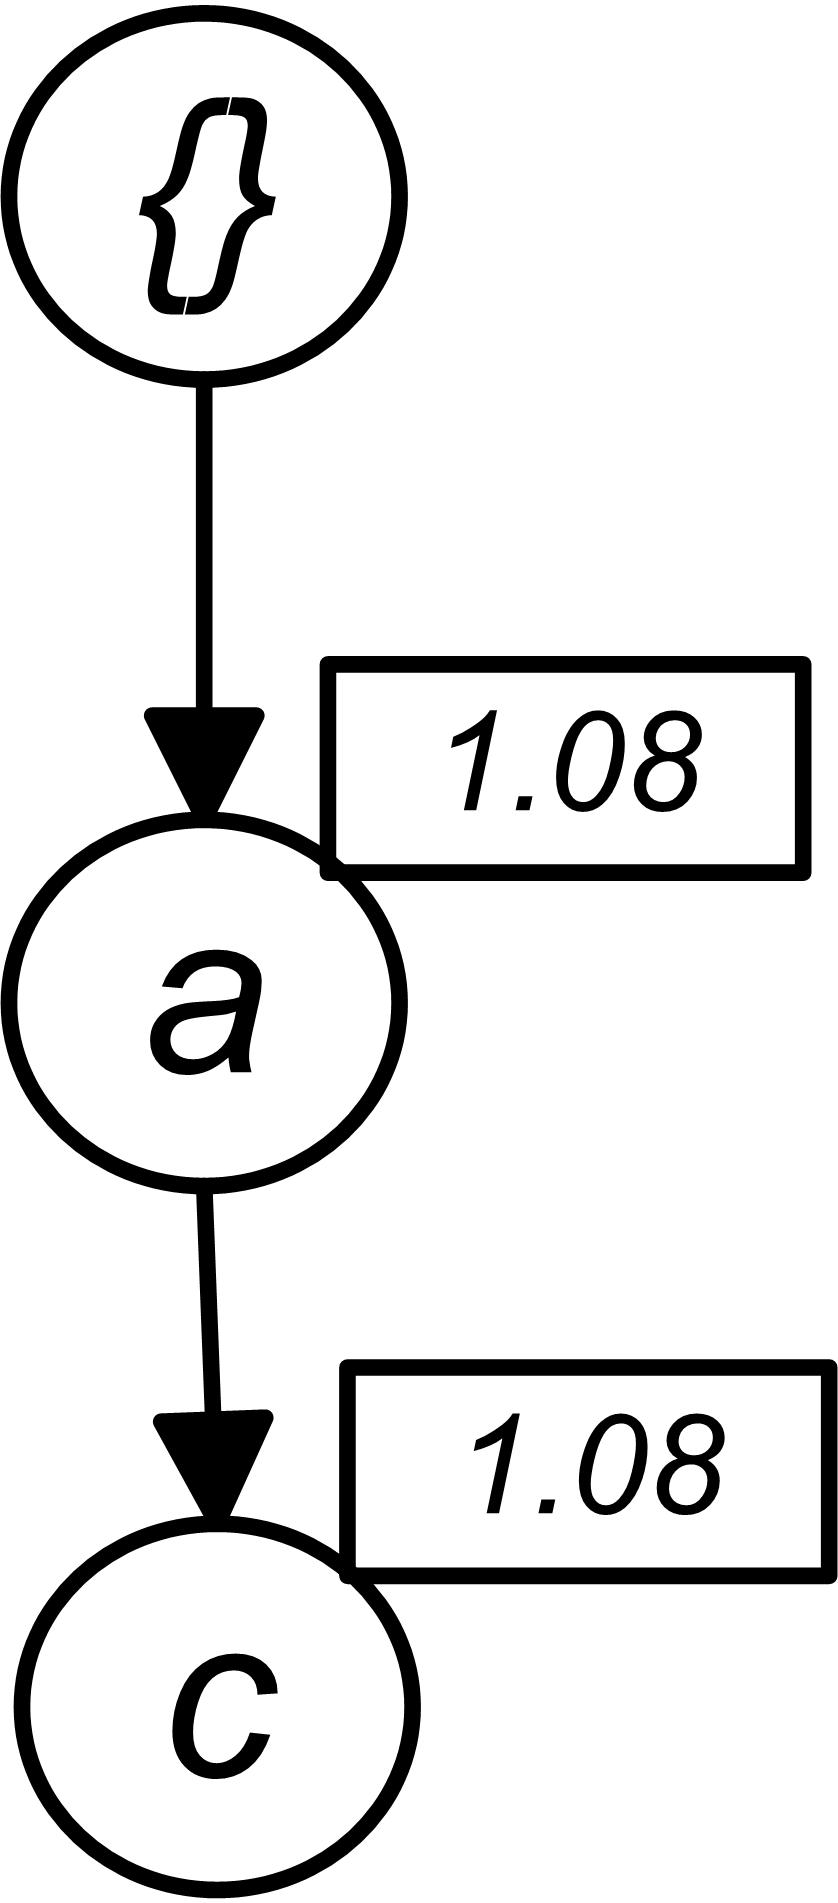
\includegraphics[width=.8\textwidth, height=5cm]{images/D_COND.jpg}
  \hfill
\end{minipage}
\hfill
\begin{minipage}{0.30\textwidth}
  \centering
  
	\begin{center}
	\begin{tabular}{ |c| } 
 	\hline
 		Freq Patterns \\ \hline\hline
 		dc  	\\ \hline
 		da   	\\ \hline
 		dca   	\\ \hline
 		
\end{tabular}
\end{center}  
  \captionof{table}{ \emph{Frequent Patterns} }
\end{minipage}
\caption{\emph{d-cond} Tree and corresponding Header}
\label{figure:d_cond}
\end{figure}
\begin{figure}
\begin{minipage}{0.30\textwidth}
  \centering
	\begin{center}
	\begin{tabular}{ |c|c| } 
 	\hline
 		Item&Value\\ \hline\hline
 		a &  .99  	\\ \hline
 		b &  .54   	\\ \hline
\end{tabular}
\end{center}  
  \captionof{table}{Header }
\end{minipage}
  \hfill
\begin{minipage}{0.29\textwidth}
  \centering
  \hfill
  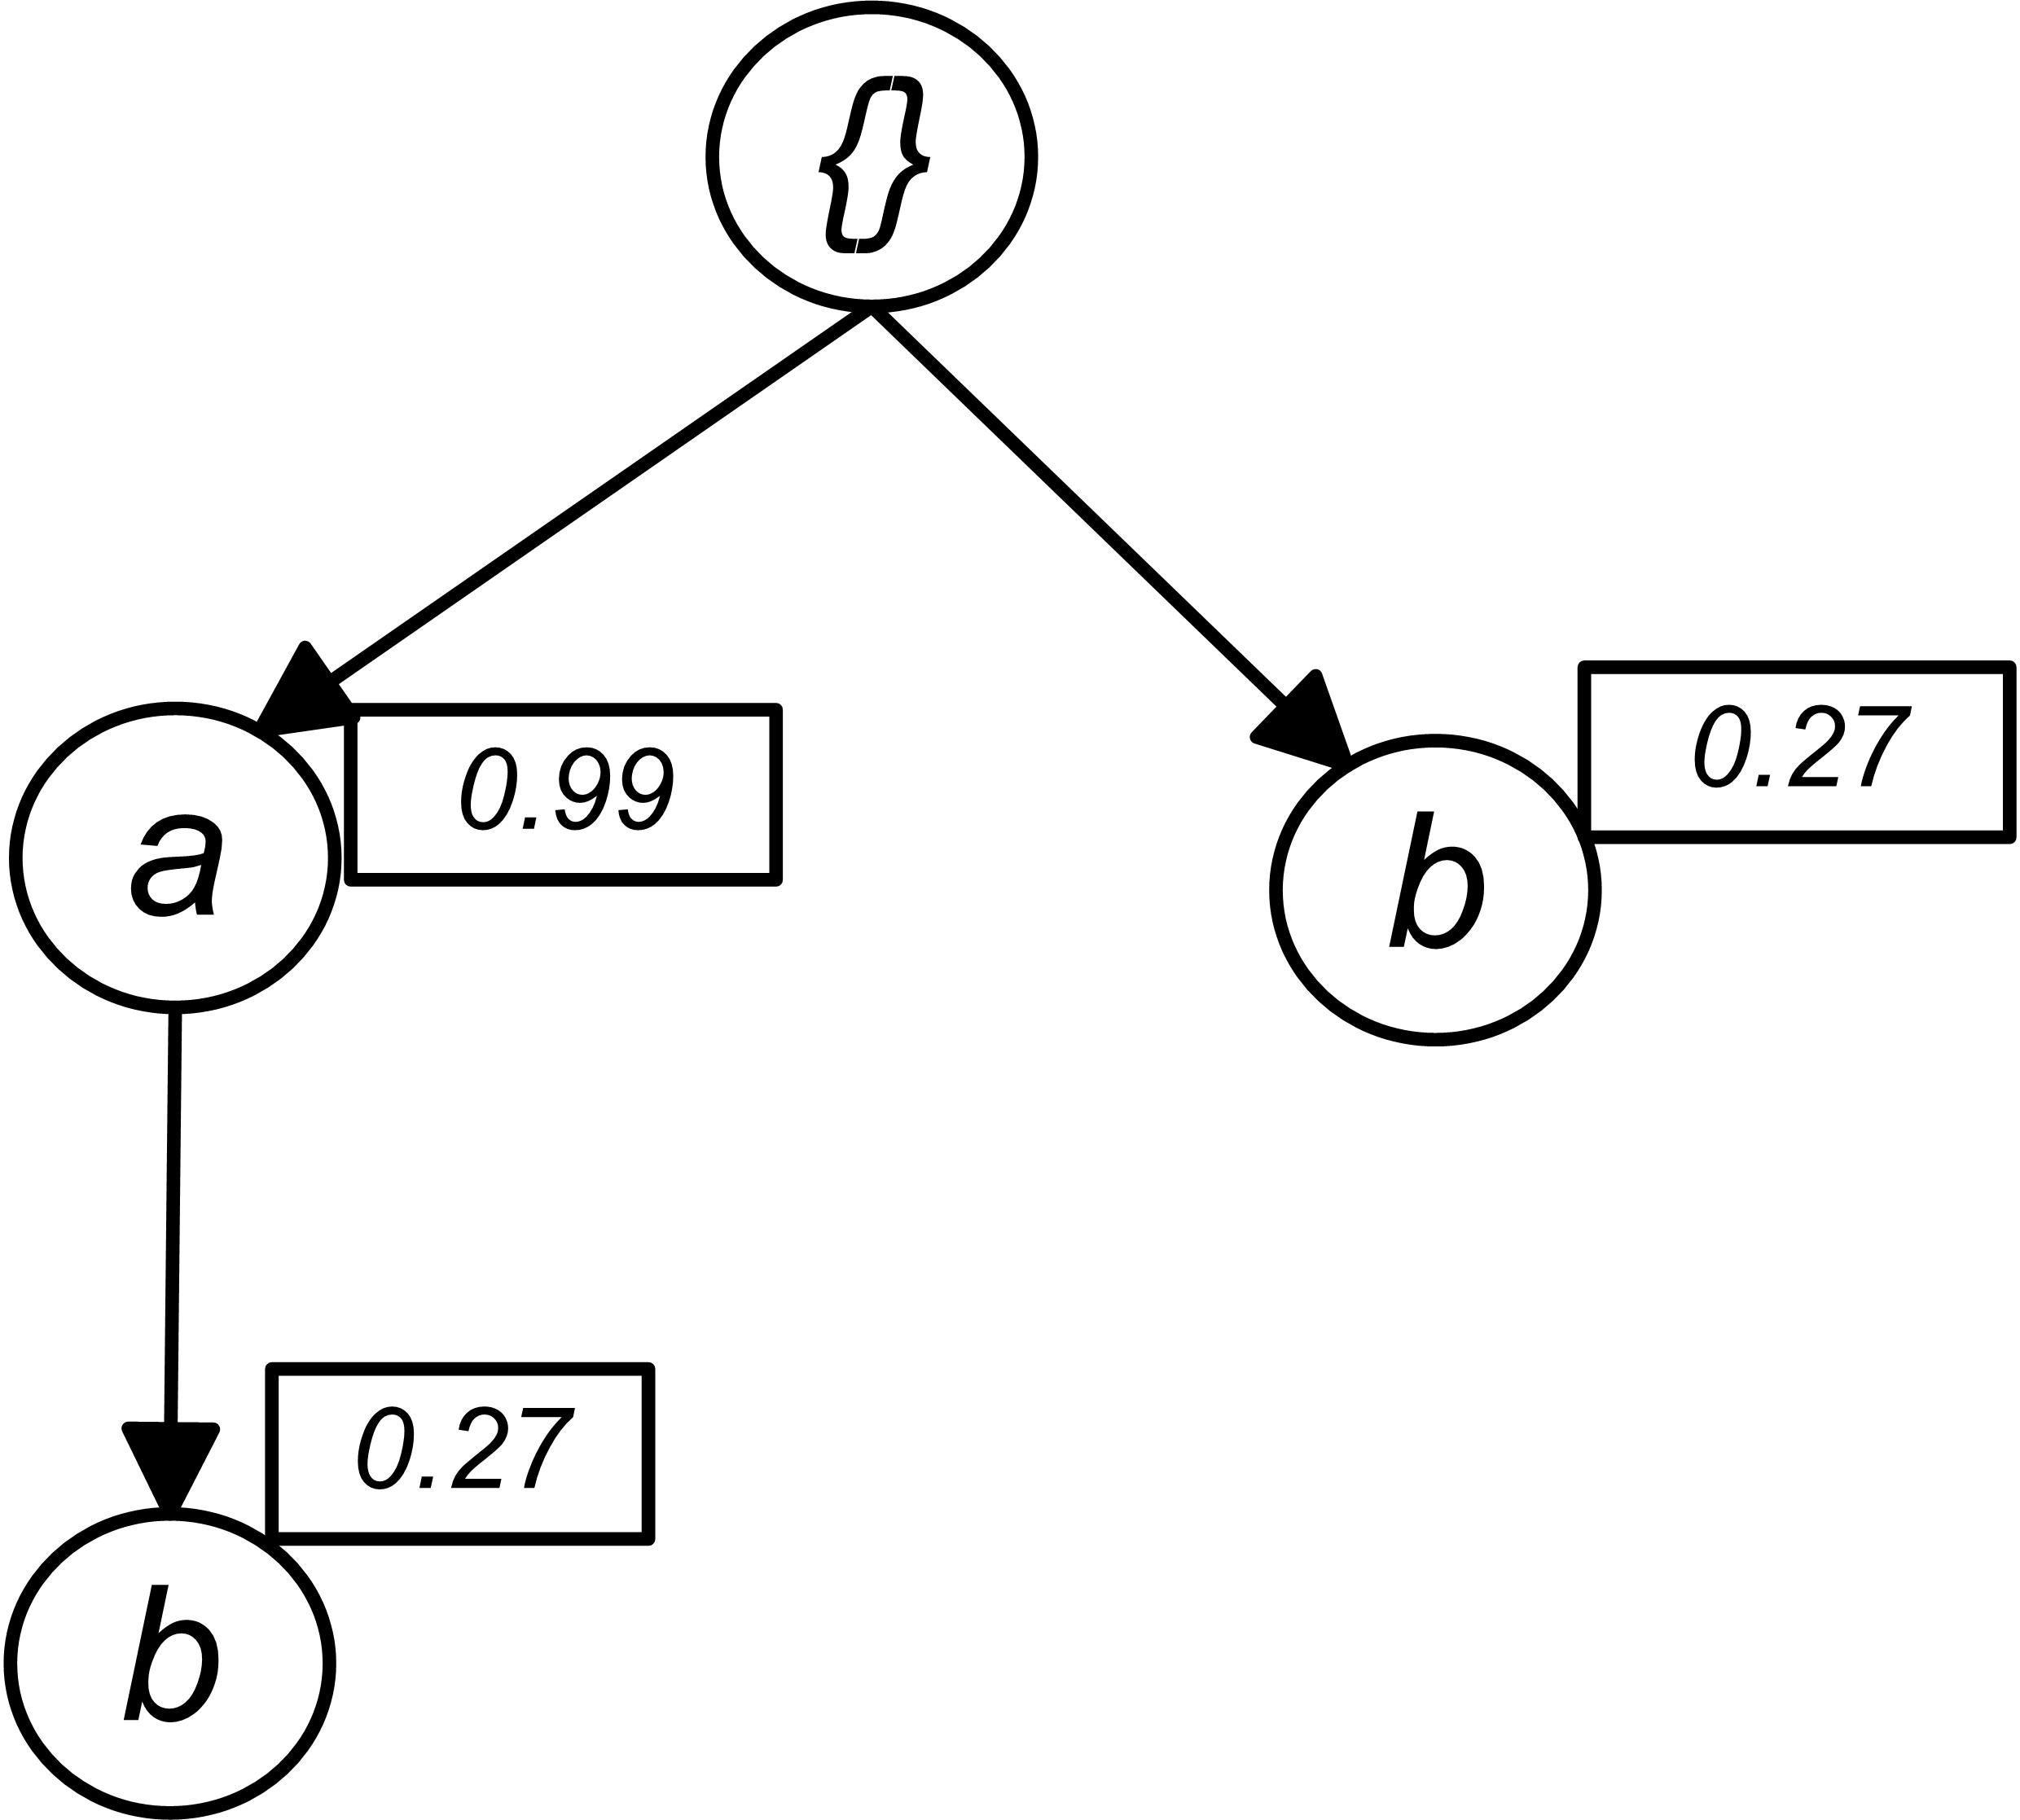
\includegraphics[width=.8\textwidth, height=3.5cm]{images/C_COND.jpg}
  \hfill  
\end{minipage}
\hfill
\begin{minipage}{0.30\textwidth}
  \centering  
	\begin{center}
	\begin{tabular}{ |c| } 
 	\hline
 		Freq Patterns \\ \hline\hline
 		ca  	\\ \hline
 		
\end{tabular}
\end{center}   
  \captionof{table}{ \emph{Freq Patterns} }
\end{minipage}
\caption{\emph{c-cond} Tree and corresponding Header}
\label{figure:c_cond}
\end{figure}
\begin{figure}
\centering
  
\includegraphics[width=.10\textwidth, height=1.1cm]{images/A_COND.jpg}
\caption{\emph{a-cond} Tree}
\label{figure:a_cond}
\end{figure}

%\end{document}

    \subsection{False positive reduction}
    False positives are such patterns those are exist in the frequent pattern list but not actually frequent. False negatives are such patterns those does not exist in the frequent pattern list but actually frequent. As our whole process of \emph{U\textsuperscript{cap}} assignment, construction of \emph{US-tree} and \emph{USFP-growth} mining algorithm, all are process are based on taking upper value of two item set supports, our process may create some false positives but no false negatives. In this section we will discuss about finding and eliminating all the false positives from found patterns from \emph{USFP-growth} mining result. For this elimination process we just use two scans of transactions. In the first scan we eliminate the infrequent one item set. In the second scan we update \emph{frequent tree} exact support that makes easily to find infrequent items if exists in our frequent item found. The process is given below.\\
    In the previous sections we described about tree construction and mining approach. Mining transaction table-\ref{table:transaction_batch} we found \emph{\{a\}, \{b\}, \{c\} \{d\}, \{dc\}, \{da\}, \{dca\}} and \emph{\{ca\}} as frequent patterns. From the patterns we first construct a pattern tree from the patterns. This tree is very much easier to construct. For tree construction we first create root node \emph{\{\}}. Then take each frequent item and insert into the root node as a child. for \emph{a}, \emph{b}, \emph{c}, \emph{d} we just insert as child as it does not exists in the tree. For \emph{dc} do not create new node for \emph{d} but create a new node \emph{c} as child of \emph{d} as there is no \emph{c} exists in the child of \emph{d}. Thus we construct the whole frequent pattern tree for further identification of infrequent patterns. \\
    Next, in the first scan of inserted transactions, we remove one item infrequent all items from transactions. Figure-\ref{figure:frequent_patterns_final} table shows the transaction table after eliminating all nodes accepts one item frequent. As for one item frequent checking we did not take any upper bound limit we get exact one item frequent patterns. From our \emph{Frequent Item Tree} all the children of \emph{root \{\}} are frequent and there is no false positive. So we can get \emph{\{a\}, \{b\}, \{c\} \{d\}} one item frequent set and without these all other items are infrequent.  Then in the second scan we take each transaction and update each nodes support. In the tree we update value with the equation-\ref{equation:exp_sup}. After scanning second time our \emph{Frequent Item Tree} becomes full fill with all information to find infrequent exists in our patterns. For this we need to traverse the \emph{Frequent Item Tree}. As the tree contains all nodes with its own support we get the true infrequent. For example, for \emph{\{d, a\}} path \emph{a : 0.89} as the actual support for {da : 0.89} pattern. We find this in frequent, so we can easily eliminate. Figure-\ref{figure:frequent_patterns_final} shows the identifying all the frequent item set infrequent. So we can eliminate all the false positives.    And find the exact frequent patterns. From the tree we find the patterns \emph{\{a\}, \{b\}, \{c\} \{d\} and \{dc\}}.
    %\documentclass{article}
%\usepackage{fixltx2e}
%\usepackage{caption}
%\usepackage{graphicx}
%\begin{document}
\begin{figure}
\begin{minipage}{0.40\textwidth}
  \centering
  
	\begin{center}
	\begin{tabular}{ |c| } 
 	\hline
 		Frequent Items\\ \hline\hline
 		a \\ \hline
 		b \\ \hline
 		c \\ \hline
 		d \\ \hline
 		dc \\ \hline
 		da \\ \hline
 		dca \\ \hline
 		ca \\ \hline
\end{tabular}
\end{center}  
  
  
  \captionof{table}{\emph{Frequent Items}}
\end{minipage}
\hfill
\begin{minipage}{0.40\textwidth}
  \centering
  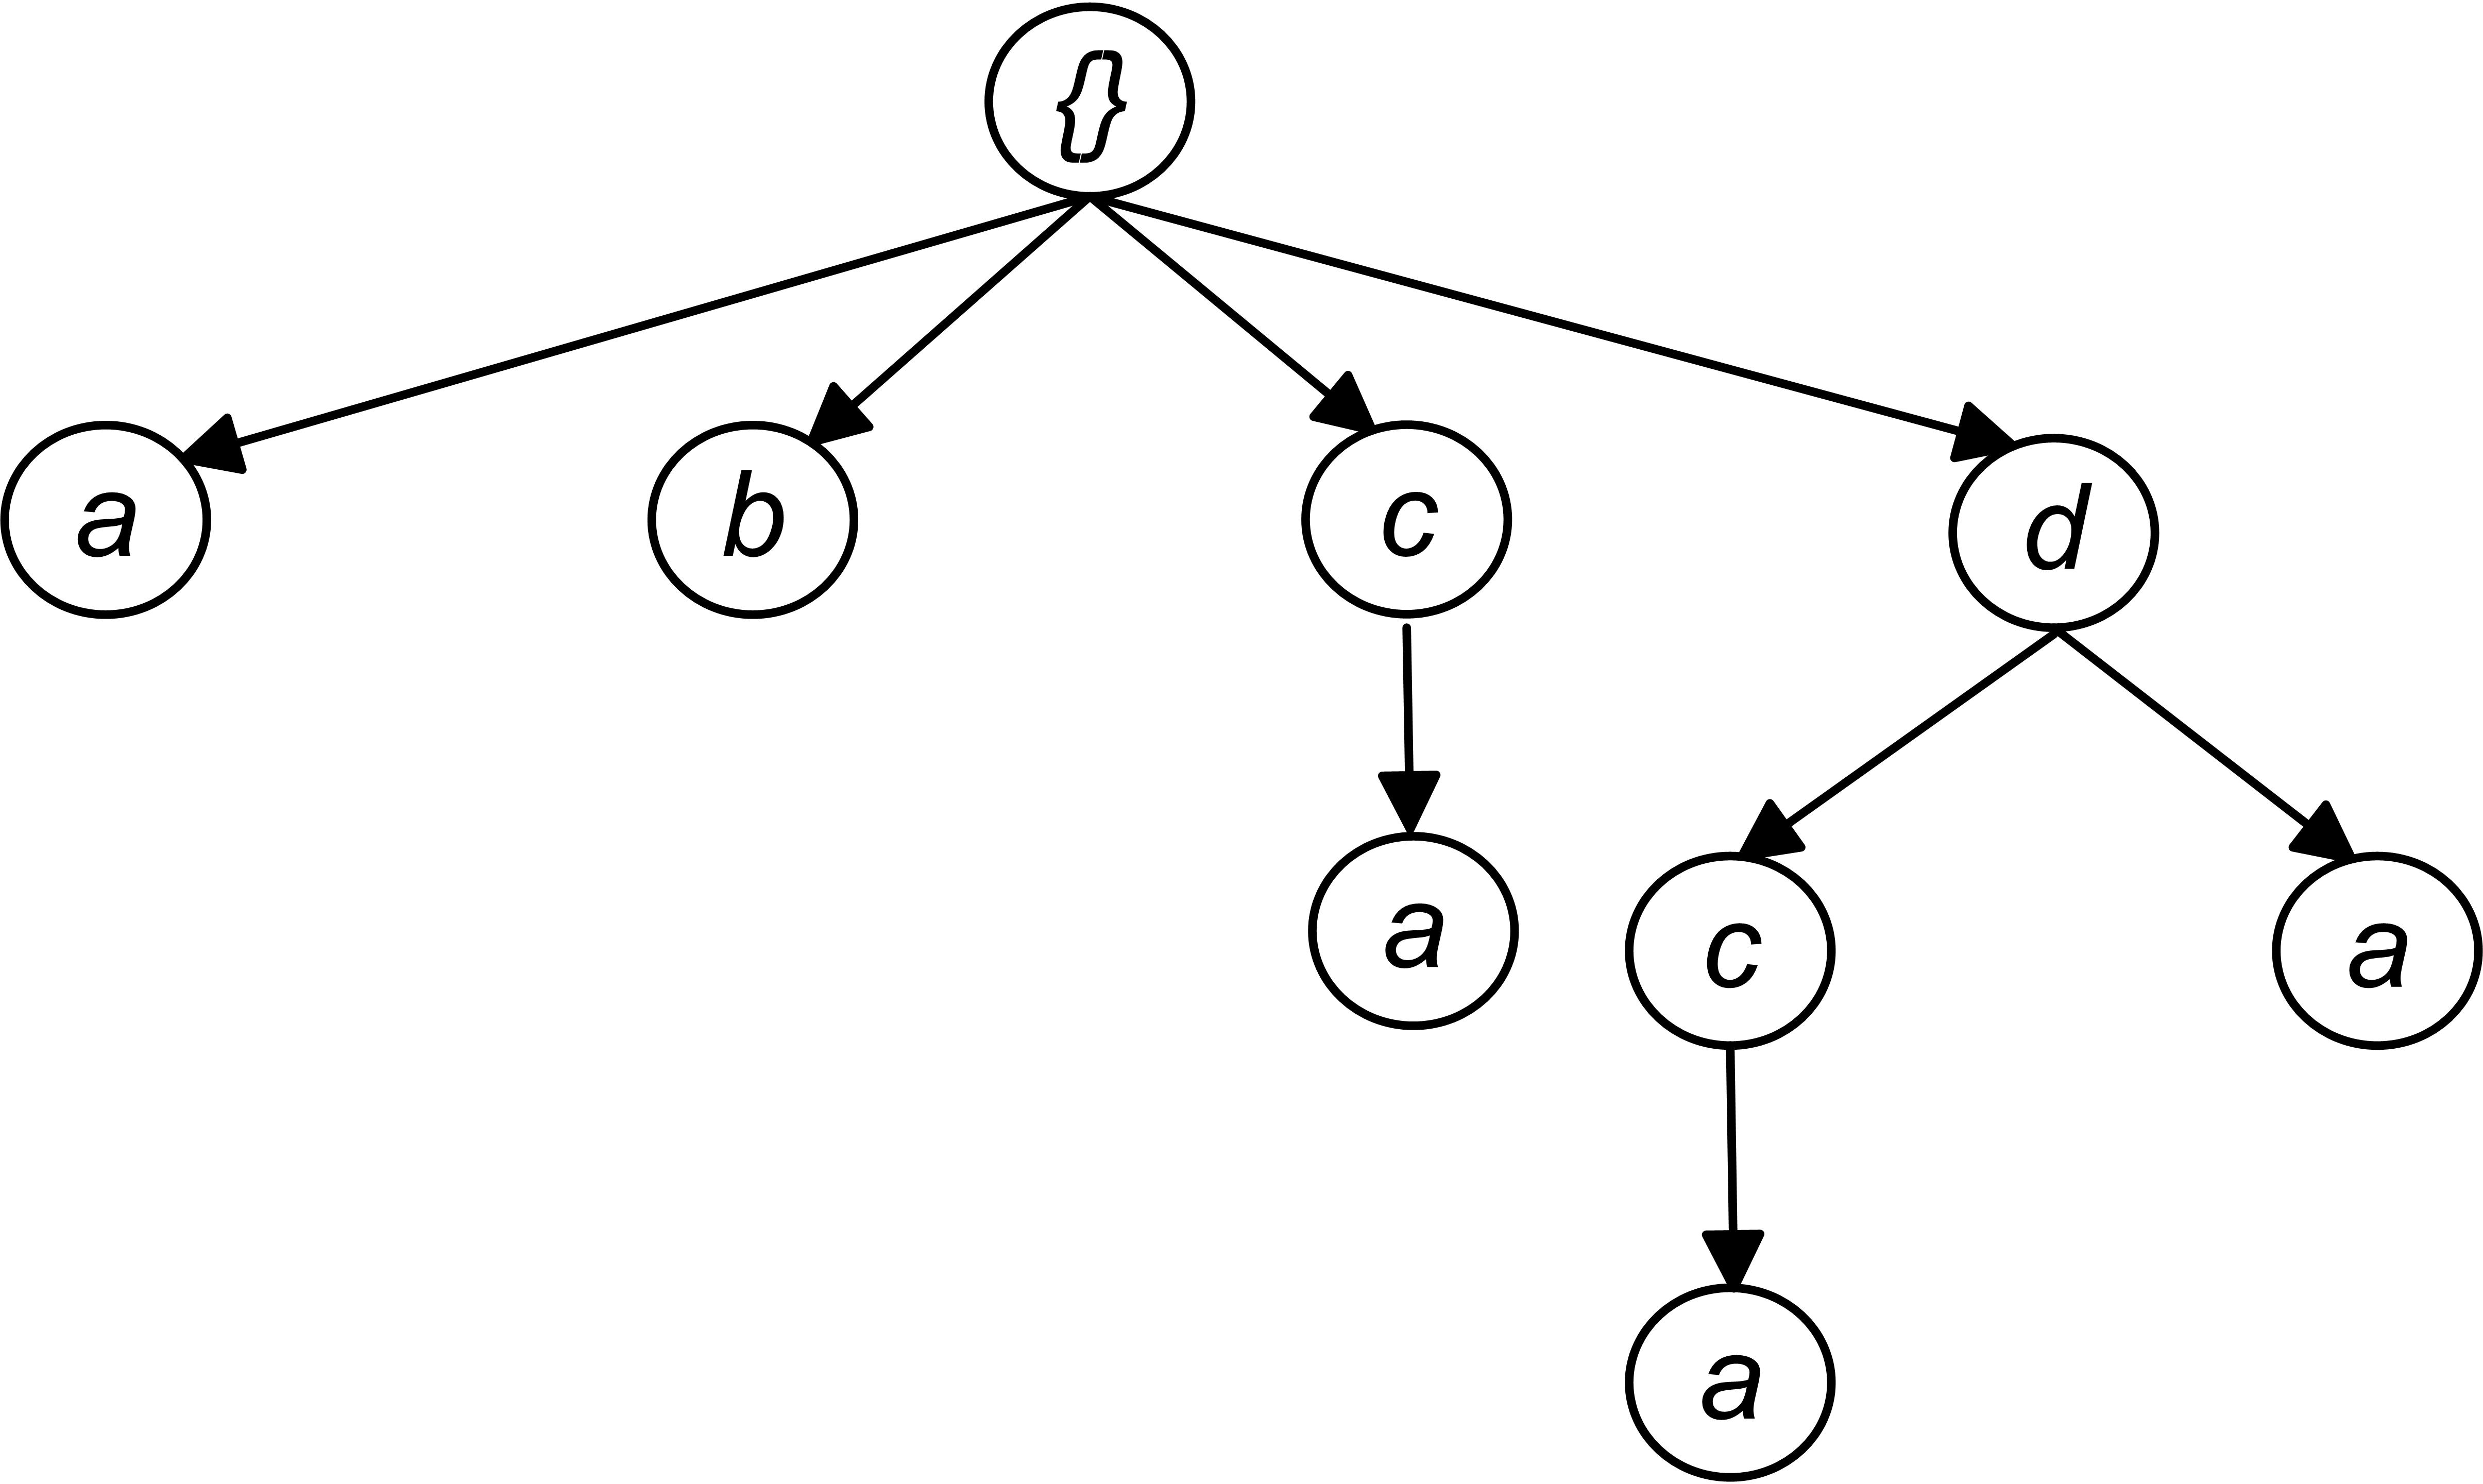
\includegraphics[width=\textwidth]{images/frequent_tree.jpg}
  \captionof{figure}{\emph{Frequent Item Tree} }
\end{minipage}
\caption{Frequent Patterns and Pattern Trees}
\label{figure:frequent_patterns}
\end{figure}
\begin{figure}
\begin{minipage}{.4\textwidth}
  \centering
  
	\begin{center}
	\begin{tabular}{ |c|c| } 
 	\hline
 		No & Items \\ \hline\hline
 		T\textsubscript{1} & \emph{a(0.9),c(0.6),d(0.5)}\\ \hline
 		T\textsubscript{2}& \emph{a(0.9),b(0.4),e(0.1)}\\ \hline
 		T\textsubscript{3}& \emph{a(0.2),c(0.9),d(0.7)}\\ \hline
 		T\textsubscript{4}& \emph{b(0.3),c(0.9)}\\ \hline
 		T\textsubscript{5}& \emph{a(0.1),b(0.3),c(0.9)} \\ \hline
 		T\textsubscript{6} & \emph{a(0.9),e(0.3)
}\\ \hline
\end{tabular}
\end{center}  
\end{minipage}
\hfill
\begin{minipage}{0.50\textwidth}
  \centering
  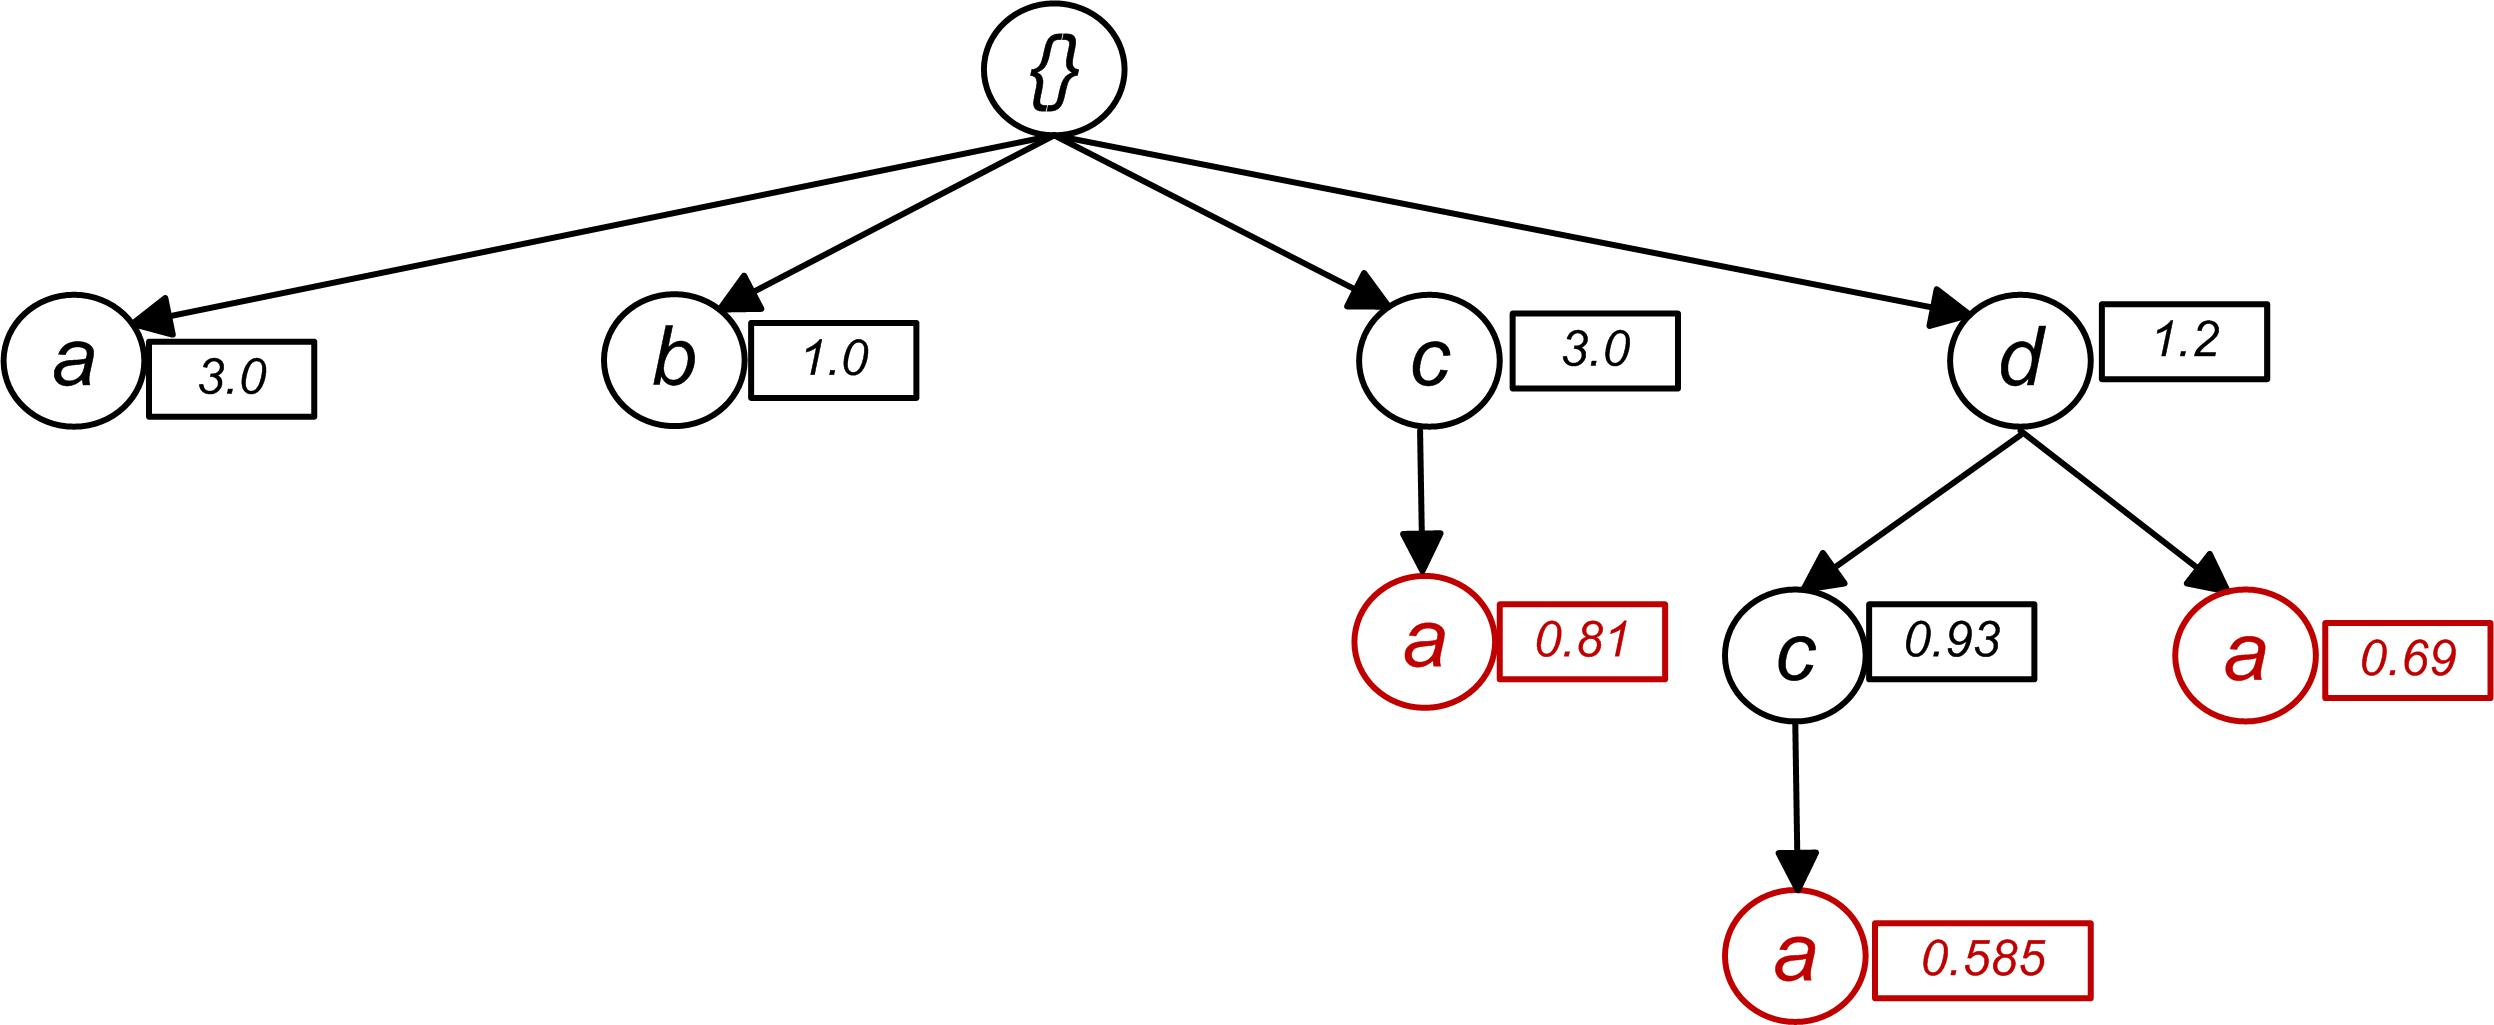
\includegraphics[width=\textwidth]{images/frequent_tree_final.jpg}
\end{minipage}
\caption{Transaction Table and Pattern Trees identifying \emph{False Positives}}
\label{figure:frequent_patterns_final}
\end{figure}
%\end{document}

\clearpage    
    \subsection{Algorithm}
    In this section we have given our proposed algorithms. First we gave algorithm-\ref{algorithm:cap_assignment} that is for I\textsuperscript{cap} calculation for each item of any transaction. Then algorithm-\ref{algorithm:tree_construction} is for \emph{US-tree} construction and algorithm-\ref{algorithm:mine} is for mining with \emph{USFP-growth} algorithm.
    %\documentclass[a4paper]{article}

%\usepackage[english]{babel}
%\usepackage[utf8]{inputenc}
%\usepackage{amsmath}
%\usepackage{amsfonts}
%\usepackage{graphicx}
%\usepackage[colorinlistoftodos]{todonotes}
%\usepackage{algorithm}
%\usepackage{algpseudocode}

%\usepackage{geometry}
% \geometry{
% a4paper,
% total={210mm,297mm},
% left=20mm,
% right=20mm,
% top=20mm,
% bottom=20mm,
% }

%\begin{document}
  \begin{algorithm}
   \caption{\emph{U\textsuperscript{cap}} Assignment}
    \begin{algorithmic}[1]
      \Function{Assign\emph{U\textsuperscript{cap}}}{$Batch$ $B$}
			\For {Transaction $T$  in Batch}
				\For {$\$i=1$ to size of ( $T$ )}
					\State $\$Item$ = T[$[i]$]
					\If{$i=1$}
						\State $\$Item$[\emph{U\textsuperscript{cap}}] $=$ $Probability(\$Item)$
					\Else
						\State $\$Item$[\emph{U\textsuperscript{cap}}] $=$ MAX \{ $Probability(\$T[1])$ to $Probability(\$T[i-1])$ \} $*$ $Probability(\$Item)$
					\EndIf
				\EndFor
			\EndFor
       \EndFunction

\end{algorithmic}
\end{algorithm}
%\end{document}
\clearpage
    \section{Summary}
    In this section, we will discuss our proposed approach for mining frequent pattern over large uncertain stream data. Stream Data has a special property that it comes and flows away. For this reason, we will lose data after data stream has flown away. To resolve this, we will propose a window based approach where we will keep the most recent information in a tree structure as the most recent data is most valuable. Later we will show how the window will slide, remove old data and insert new data in the window. As, for uncertain data stream each same item in the different transaction has different existential probability, it becomes very hard to merge (share) this node in the tree. This uncertainty property of item makes the tree huge. We have proposed a new \emph{U\textsuperscript{cap}} value for each item that helps to share a single node when constructing the tree which we named as \emph{US-tree}. We will show that our proposed tree \emph{US-tree} will be very compact and very efficient for later mining. Later, will describe an approach for mining the \emph {US-tree} named \emph{USFP-growth} which is \emph{FP-growth} like approach. Later we will propose a method for filtering false positive from finding most probable frequent patterns.
%\end{document}
 % Proposed Approach
%%%
%\documentclass[a4paper,12pt]{book}
%\usepackage{pgfplots}
%\usepackage[justification=centering]{caption}
%\pgfplotsset{compat=newest}
%\begin{document}
\chapter{Experimental Results}
\lhead{Chapter 4. \emph{Experimental Results}}
In this chapter we have shown our experimental results achieved by our proposed approach. Based on several performance metric we have tried to show our algorithms' efficiency and performance. We have taken different scale/parameter to evaluate our algorithm


\section{Experimental Settings}
We have performed number of simulations in our experiment on both synthetic database and real world database. The data are taken from data set repository ~\cite{dataset}. Our experiment shows that \emph{US-tree} ( Uncertain Stream tree )is very much compact. This tree construction technique can make the items to share one node. This compactness of \emph{US-tree} surprisingly helps the mining, \emph{USFP-growth} ( Uncertain Stream Frequent Pattern growth ) process to gain a lot in run-time and memory. More over our proposed pattern tree can be used to find max patterns and close patterns. Performance tests from our experiment shows that \emph{US-tree} tree construction technique and \emph{USFP-growth} mining algorithm can run on any uncertain stream database with any support threshold, window size and batch size. Our experimental result shows that these techniques are much more faster and scalable frequent pattern mining technique. As we have proposed a new approach for finding frequent patterns over uncertain data we have compared performance with itself for comparing correctness of our approach. Then we have compared with all well known existing approaches for finding frequent item sets over uncertain database. \emph{SUF-growth} is one of them. We have tried to compare in all aspects to prove our approach's correctness, run-time efficiency and memory efficiency.
%\documentclass{article} 
%
%\begin{document}
\begin{table}
\centering

\begin{tabular}{|l|l|}
\hline 
	Property&Configurations\\ \hline\hline

	Processor				& Intel(R) Core(TM) i7		\\ \hline
	Core Count				& 8							\\\hline
	Memory					& 8 GB RAM 					\\\hline
	OS Name					& Windows					\\ \hline
	OS version 				& 7, service pack 1 		\\ \hline
	OS Architecture 		& 64 bit					\\ \hline
	Programming Language 	& Java						\\ \hline
	Development Kit 		& JDK						\\ \hline
	Development Kit Version & 1.7 SE.					\\\hline
	Virtual Machine 		& JVM						\\ \hline
	Runtime Environment 	& JRE 7						\\\hline
	Build Tool				& Gradle					\\\hline
	Build Tool Version		& 2.6						\\\hline
	\end{tabular}
\caption{Configuration of Experimental Environment}
\label{table:experiment_configuration}
\end{table}
%\end{document}
All program for the simulating experimental result are written \emph{Java} programming language that run on \emph{Java Run time Environment (JRE) - 1.7.0.79}. All program was run on a computer having \emph{3.4 GHz Intel(R) Core(TM) i-7} processor and \emph{8 GB RAM} with \emph{Windows-7, 64-bit, service pack-1} operating system installed in it (Table-[\ref{table:experiment_configuration}]). For management of the experimental project Gradle was used as build tool. Results shown in this chapter are based on average of multiple run for every case. \emph{US-tree} was constructed with chronological order of database items. All the running time includes \emph{CPU}, \emph{I/O}.\\
\documentclass{article}
\usepackage{pgfplots}
\begin{document}
\pgfmathdeclarefunction{gauss}{2}{%
  \pgfmathparse{1/(#2*sqrt(2*pi))*exp(-((x-#1)^2)/(2*#2^2))}%
}
\begin{figure}
\centering
\begin{tikzpicture}
\begin{axis}[
 width=11cm,
   height=8cm,
  no markers, domain=0:1, samples=1000,
  axis lines*=left, xlabel=Items, ylabel=Uncertaininty Value,
%  every axis y label/.style={at=(current axis.above origin),anchor=south},
  every axis x label/.style={at=(current axis.right of origin),anchor=west},
  height=5cm, width=12cm,
  xtick={.5}, ytick=\empty,
  enlargelimits=false, clip=false, axis on top,
  grid = major
  ]

  \addplot [thick,cyan!50!blue] {gauss(.5,.159154943)};
\end{axis}

\end{tikzpicture}
\caption{Normal Distribution}
\label{result:normal_distribution}
\end{figure}
\end{document}
we got the synthetic and real life datasets from the frequent itemset mining repository ~\cite{dataset}, those were collected for certain databases. Then we have used our own probabilistic tool and technique to generate existential probability of each items of the each transaction of database. Real life data set actually follows Gaussian distribution that is normal distribution [\ref{result:normal_distribution}]. It actually says that in real world extreme cases are minimum and average case are maximum. From the figure [\ref{result:normal_distribution}] we can see that in the middle the pick value is highest so we can say count item probability at \emph{.5} is maximum. So we used this technique to generate and introduce existential probability to each items in a transaction. We have used \emph{Java pseudo random} generate existential probability for each item of all the transaction of database. By assigning these probability value to each items we have generate uncertain database for both real life database and synthetic database found from dataset repository ~\cite{dataset}. However one can give existential probability by any distribution according to need.


\section{Performance Metrics}
We have consider several metrics as parameters for evaluating our proposed algorithm. We have set several property for this evaluation from experimental result. As we have worked on data set that comes like stream so we have set parameters for both the frequent item set mining from total data set and per window. The parameters and properties are given below:

\begin{itemize}
	\item {Correctness}
	\begin{itemize}
		\item batch size vs running time.
		\item window size vs running time.
		\item transactions in a window vs false positive count.
	\end{itemize}
	\item {Comparison with existing approaches}
	\begin{itemize}
		\item Tree construction time per window and total database vs minimum support.
		\item Mining time per window and total database vs minimum support.
		\item Total time to complete per window and total database vs minimum support.
		\item Total tree node in tree per window vs minimum support.
		\item Total memory needed by mining process vs minimum support.
	\end{itemize}
\end{itemize}
\section{Experimental Environment}
For our experimental evaluation we used both real life database and synthetic database from database repository ~\cite{dataset}. Table [\ref{table:dataset}] shows the data base type and properties.
		\begin{table}[h]
		\centering
		\begin{tabular}{|c|c|c|c|c|}
		\hline 
		Name		&	Type	&	Density	&	Total Transaction 	&	Distinct Items	\\ \hline \hline
		mushroom	&	real	&	dense	&	8124	&	120							\\ \hline
		kosarak		&	real	&	sparse	&	990002	&	41270						\\ \hline
		pumsb star	&	real	&	sparse	&	49046	&	2088						\\ \hline
		chess		&	real	&	dense	&	3196	&	75							\\ \hline
		T10I4D100K	&	synthetic	&	sparse	&	100000	&	869						\\ \hline
			\end{tabular}
		\caption{Dataset from repository ~\cite{dataset}}
		\label{table:dataset}
		\end{table}


\subsection{Real Life Data Set}
For real life data sets we have used mushroom ~\cite{dataset} and chess ~\cite{dataset}. Mushroom, chess and pumsb star are dense datasets. Mushroom has 8124 transactions with 120 distinct items and chess has 3196 transactions with 75 distinct items. For probability assignment to each items we used normal distribution for getting existential probability. For giving existential probability to each item of each transaction in database we have followed the natural distribution described earlier. Figure \ref{result:g_dataset_mushroom}, figure \ref{result:g_dataset_chess} shows the probability distribution for corresponding mushroom and chess.
		\begin{figure}[h]
		\centering
			%%mark = star, diamond, square, otimes
%\documentclass{article}
%\usepackage{pgfplots}
%\usepackage[justification=centering]{caption}
%\pgfplotsset{compat=newest}
%\begin{document}
\begin{figure}
\centering

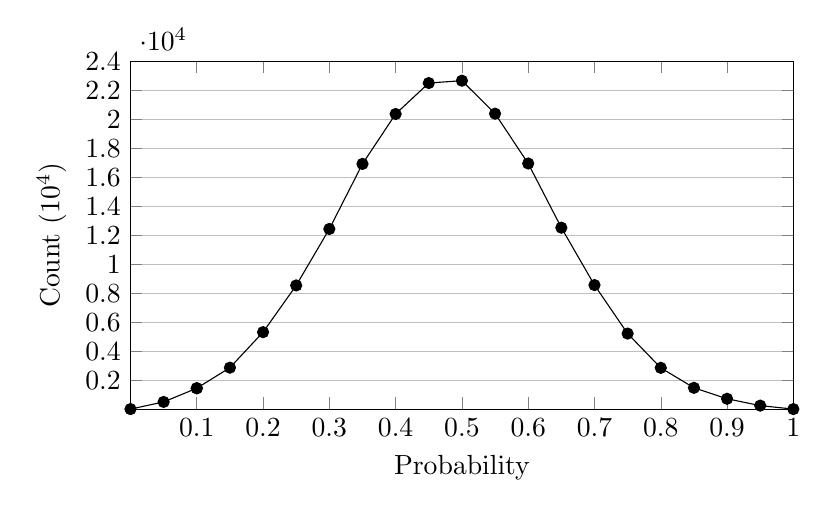
\begin{tikzpicture}
\begin{axis}[
 width=10cm,
   height=6cm,
    xlabel={Probability },
    ylabel={Count ($10^4$)},
    xmin=0, xmax=1.0,
    ymin=0, ymax=24000,
    xtick={.1,.2,.3,.4,.5,.6,.7,.8,.9,1.0},
    ytick={2000,4000,6000,8000,10000,12000,14000,16000,18000,20000,22000,24000},
    legend pos=north east,
    ymajorgrids=true,
    grid style={line width=.2pt,draw=gray!50},
]
 
\addplot[
    solid, every mark/.append style={solid, fill=black}, mark=*
    ]
    coordinates {
		(0,0)
		(.05,495)
		(0.1,1439)
		(0.1 ,1439)
		(0.15,2859)
		(0.2 ,5307)
		(0.25,8531)
		(0.3 ,12426)
		(0.35,16915)
		(0.4 ,20358)
		(0.45,22493)
		(0.5 ,22655)
		(0.55,20380)
		(0.6 ,16943)
		(0.65,12514)
		(0.7 ,8555)
		(0.75,5209)
		(0.8 ,2845)
		(0.85,1468)
		(0.9 ,712)
		(0.95,240)
		(1.0,0)
};
 
\end{axis}
\end{tikzpicture}
%\caption{Probability Distribution for \emph{Mushroom} data set}
\label{result:data_mushroom}
\end{figure}
%\end{document}
		\caption{Probability Distribution for Mushroom ~\cite{dataset} Dataset}
		\label{result:g_dataset_mushroom}
		\end{figure}
		
		\begin{figure}[h]
		\centering
			%%mark = star, diamond, square, otimes
%\documentclass{article}
%\usepackage{pgfplots}
%\usepackage[justification=centering]{caption}
%\pgfplotsset{compat=newest}
%\begin{document}
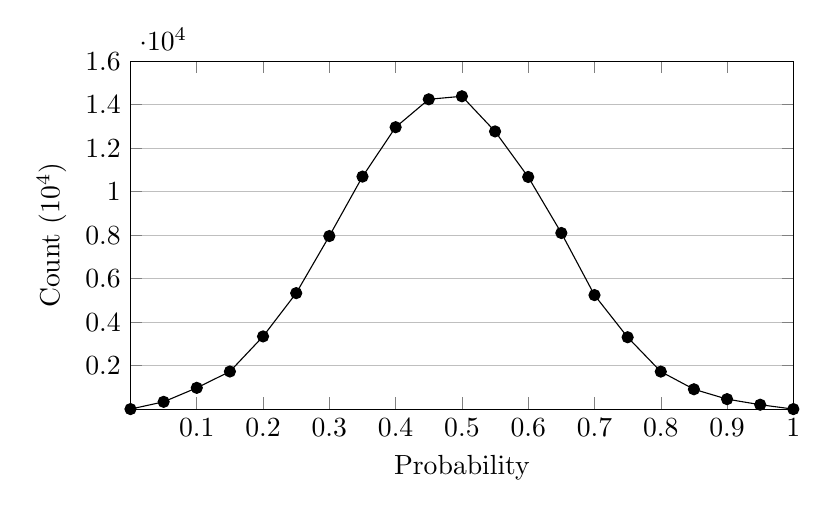
\begin{tikzpicture}
\begin{axis}[
 width=10cm,
   height=6cm,
    xlabel={Probability },
    ylabel={Count ($10^4$)},
    xmin=0, xmax=1.0,
    ymin=0, ymax=16000,
    xtick={.1,.2,.3,.4,.5,.6,.7,.8,.9,1.0},
    ytick={2000,4000,6000,8000,10000,12000,14000,16000},
    legend pos=north east,
    ymajorgrids=true,
    grid style={line width=.2pt,draw=gray!50},
]
 
\addplot[
    solid, every mark/.append style={solid, fill=black}, mark=*
    ]
    coordinates {
			(0,0)
			(0.05,334)
			(0.1,977)
			(0.15,1729)
			(0.2,3342)
			(0.25,5333)
			(0.3,7958)
			(0.35,10692)
			(0.4,12964)
			(0.45,14247)
			(0.5,14386)
			(0.55,12770)
			(0.6,10675)
			(0.65,8099)
			(0.7,5242)
			(0.75,3304)
			(0.8,1724)
			(0.85,912)
			(0.9,458)
			(0.95,201)
			(1,0)

};
 
\end{axis}
\end{tikzpicture}
%\end{document}
		\caption{Probability Distribution for Chess ~\cite{dataset} Dataset}
		\label{result:g_dataset_chess}
		\end{figure}

\subsection{Synthetic Data Set}
For synthetic data sets we have used T10I4D100K ~\cite{dataset}. It is an IBM generated transaction data set widely used for frequent pattern mining. It is a sparse data set with 100000 transactions and 869 distinct items. For probability assignment to each items we used normal distribution for getting existential probability.
		\begin{figure}[h]
		\centering
			%mark = star, diamond, square, otimes
%\documentclass{article}
%\usepackage{pgfplots}
%\usepackage[justification=centering]{caption}
%\pgfplotsset{compat=newest}
%\begin{document}
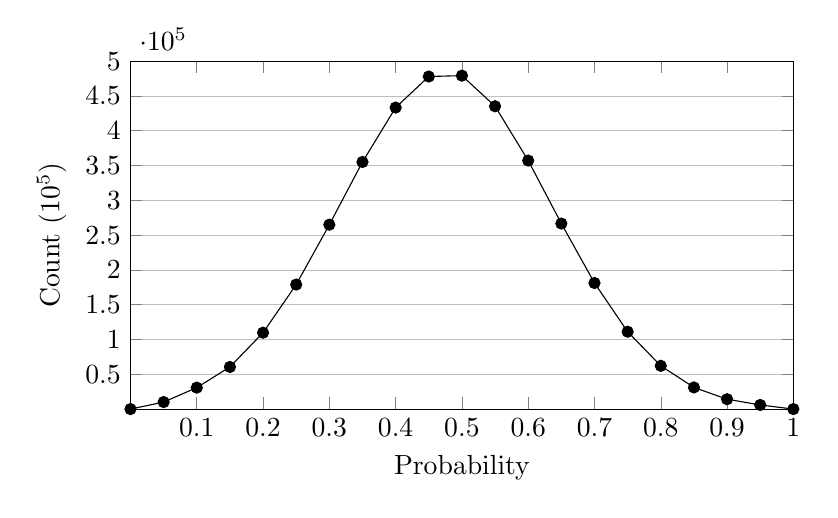
\begin{tikzpicture}
\begin{axis}[
 width=10cm,
   height=6cm,
    xlabel={Probability },
    ylabel={Count ($10^5$)},
    xmin=0, xmax=1.0,
    ymin=0, ymax=500000,
    xtick={.1,.2,.3,.4,.5,.6,.7,.8,.9,1.0},
    ytick={50000,100000,150000,200000,250000,300000,350000,400000,450000,500000},
    legend pos=north east,
    ymajorgrids=true,
    grid style={line width=.2pt,draw=gray!50},
]
 
\addplot[
    solid, every mark/.append style={solid, fill=black}, mark=*
    ]
    coordinates {
			(0,0)
			(0.05,10068)
			(0.1,30825)
			(0.15,60529)
			(0.2,109792)
			(0.25,178975)
			(0.3,265006)
			(0.35,355127)
			(0.4,433334)
			(0.45,477961)
			(0.5,479225)
			(0.55,435233)
			(0.6,357179)
			(0.65,266639)
			(0.7,181169)
			(0.75,111182)
			(0.8,62178)
			(0.85,31116)
			(0.9,14207)
			(0.95,5909)
			(1,0)
};
 
\end{axis}
\end{tikzpicture}
%\end{document}
		\caption{Probability Distribution for T40I10D100K ~\cite{dataset} Dataset}
		\label{result:g_dataset_t10}
		\end{figure}
		
		
\clearpage
\section{Comparison and Analysis}
	In this section we have provided experiment analysis. In the experiment we have focused on (1) correctness of our proposed algorithm and (2) the comparison with existing algorithm SUF-growth ~\cite{suf_growth}. For the extensive experiment we have choose mushroom dataset ~\cite{dataset} and T40I10D100K database. The reason we have choose these two dataset is, mushroom ~\cite{dataset} is real life dataset and dense dataset whereas T40I10D100K ~\cite{dataset} is synthetic and sparse dataset generated by a generator from the IBM Almaden Quest. Table \ref{table:dataset} shows the details the properties for dataset ~\cite{dataset}. Later we have also took chess ~\cite{dataset} for comparison with algorithm. The experimental results have been given in the following subsections.
\subsection{Algorithm Performance Analysis}
	\paragraph{Total Database Size Change Effect}Our experiment shows clearly that our proposed tree construction algorithm \emph{US-tree}, tree mining algorithm \emph{USFP-growth} works nicely with any size of window, batch or transaction size. For Different size of database (transaction count in a tree) this algorithm works extensively. Figure \ref{result:g_m_const_tran} shows the total running time (includes tree construction, mining and false positive reduction) change with the growth of size of mushroom dataset ~\cite{dataset}. Figure \ref{result:g_t10_const_tran} the same characteristic for T40I10D100K dataset ~\cite{dataset}. Figure \ref{result:g_m_const_tran_mem} and figure \ref{result:g_t10_const_tran_mem} shows the total nodes change in a tree while the size of database grows for databases corresponding to mushroom and T40I10D100K database. The growth of the graphs is very much regular. From these graphs it is clearly visible that, with the growth of total transaction the time increases and this certainly proves the scalability of our algorithm. 
		%%%%%%%%%%%%%%%%%%%%%%%%%%%%%%%%%%%%%%%%%%%%%%%%%%%%%%%%%%%%%%%%%%%%%%%%%%%%%%%%%%%%%%%%%%%%%%%%%%%%%%%%%%%%%%%%%%%%%%%%%%%%%%%%%%%%%%%%%%%%%%%%%%%%%%%%%%%%%%%%%%%%%%%%%%%%%%%%%%%%%%%%%%%%%%%%%%%%%%%%%%%%%%%%%%%%%%%%%%%%%
		\begin{figure}[h]
		\centering
			%mark = star, diamond, square, otimes
%\documentclass{article}
%\usepackage{pgfplots}
%\usepackage[justification=centering]{caption}
%\pgfplotsset{compat=newest}
%\begin{document}
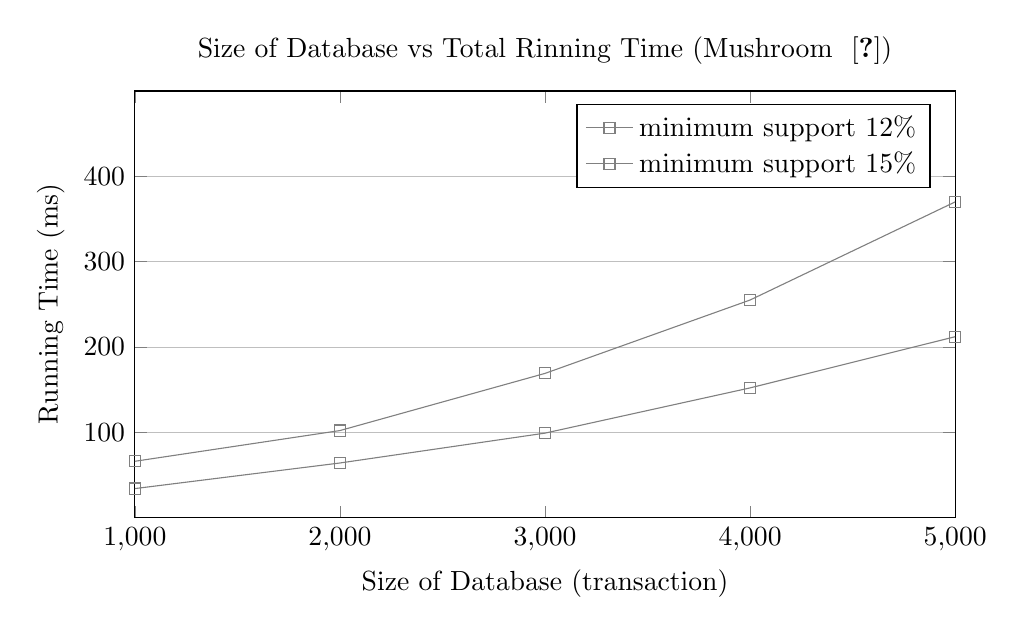
\begin{tikzpicture}
\begin{axis}[
	title={Size of Database vs Total Rinning Time (Mushroom ~\cite{dataset})},
	width=12cm,
	height=7cm,
    xlabel={Size of Database (transaction)},
    ylabel={Running Time (ms)},
    xmin=1000, xmax=5000,
    ymin=0, ymax=500,
    xtick={1000,2000,3000,4000,5000},
    ytick={100,200,300,400},
    legend pos=north east,
    ymajorgrids=true,
    grid style={line width=.2pt,draw=gray!50},
]
 
\addplot[
    solid,color=gray, every mark/.append style={solid, fill=gray}, mark=square
    ]
    coordinates {
		(1000,34)
		(2000,64)
		(3000,99)
		(4000,152)
		(5000,212)

	};
    \addlegendentry{minimum support 12\%}
	
\addplot[
    solid,color=gray, every mark/.append style={solid, fill=gray}, mark=square
    ]
    coordinates {
		(1000,66)
		(2000,102)
		(3000,169)
		(4000,255)
		(5000,370)

	};
    \addlegendentry{minimum support 15\%}

\end{axis}
\end{tikzpicture}
%\end{document}
		\caption{Size of Database vs Running Time for Mushroom Dataset ~\cite{dataset}}
		\label{result:g_m_const_tran}
		\end{figure}
		\begin{figure}[h]
		\centering
			%mark = star, diamond, square, otimes
%\documentclass{article}
%\usepackage{pgfplots}
%\usepackage[justification=centering]{caption}
%\pgfplotsset{compat=newest}
%\begin{document}
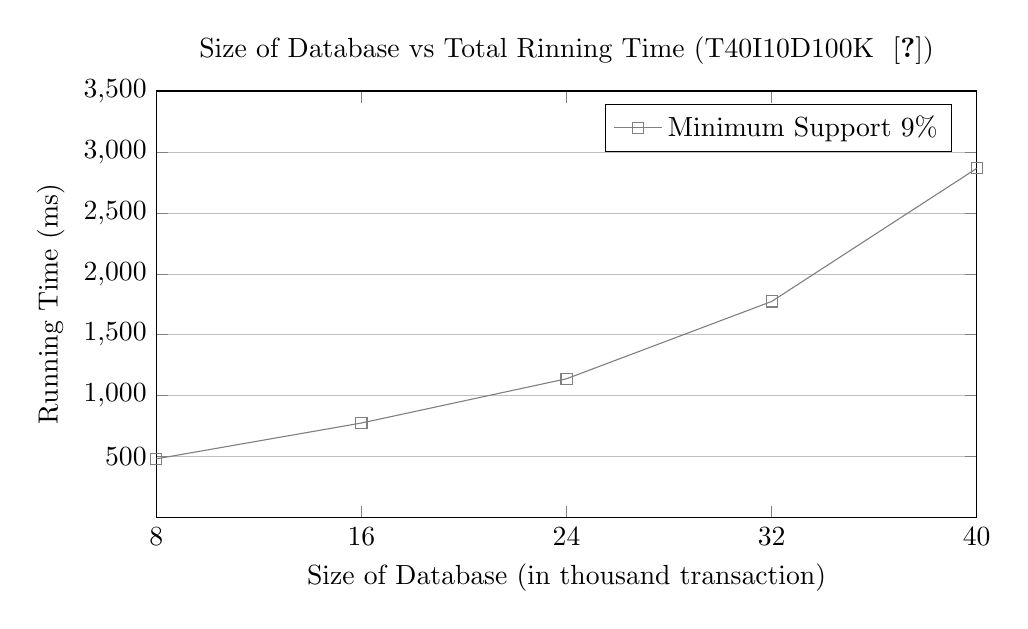
\begin{tikzpicture}
\begin{axis}[
	title={Size of Database vs Total Rinning Time (T40I10D100K ~\cite{dataset})},
	width=12cm,
	height=7cm,
    xlabel={Size of Database (in thousand transaction)},
    ylabel={Running Time (ms)},
    xmin=8, xmax=40,
    ymin=0, ymax=3500,
    xtick={8,16,24,32,40},
    ytick={500,1000,1500,2000,2500,3000,3500},
    legend pos=north east,
    ymajorgrids=true,
    grid style={line width=.2pt,draw=gray!50},
]
 
\addplot[
    solid,color=gray, every mark/.append style={solid, fill=gray}, mark=square
    ]
    coordinates {
			(8,482)
			(16,776)
			(24,1139)
			(32,1773)
			(40,2865)

	};
    \addlegendentry{Minimum Support 9\%}

\end{axis}
\end{tikzpicture}
%\end{document}
		\caption{Size of Database vs Running Time for T40I10D100K Dataset ~\cite{dataset}}
		\label{result:g_t10_const_tran}
		\end{figure}
		%%%%%%%%%%%%%%%%%%%%%%%%%%%%%%%%%%%%%%%%%%%%%%%%%%%%%%%%%%%%%%%%%%%%%%%%%%%%%%%%%%%%%%%%%%%%%%%%%%%%%%%%%%%%%%%%%%%%%%%%%%%%%%%%%%%%%%%%%%%%%%%%%%%%%%%%%%%%%%%%%%%%%%%%%%%%%%%%%%%%%%%%%%%%%%%%%%%%%%%%%%%%%%%%%%%%%%%%%%%%%
		\begin{figure}[h]
		\centering
			%mark = star, diamond, square, otimes
%\documentclass{article}
%\usepackage{pgfplots}
%\usepackage[justification=centering]{caption}
%\pgfplotsset{compat=newest}
%\begin{document}
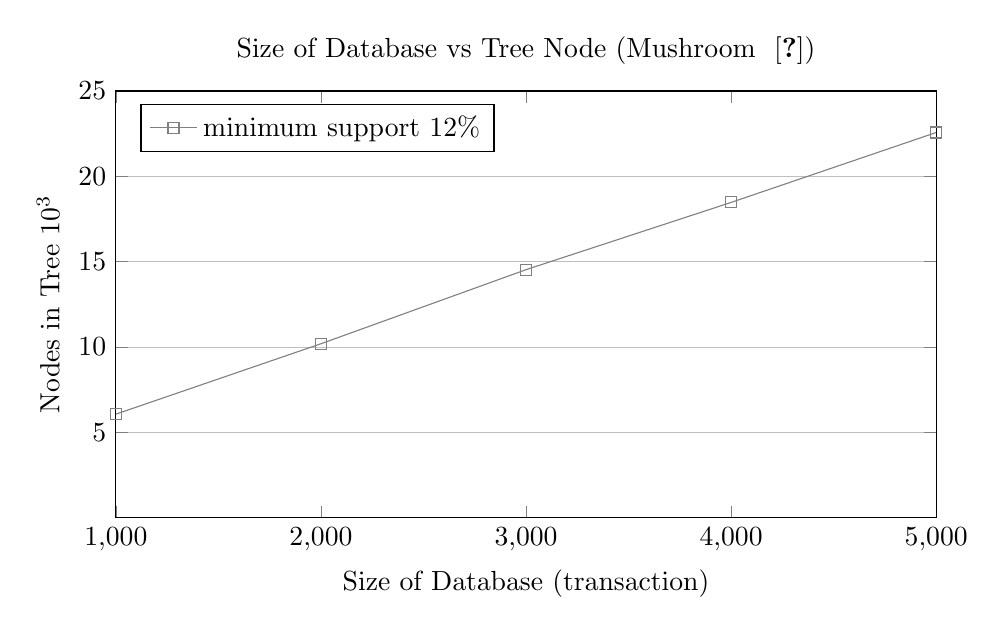
\begin{tikzpicture}
\begin{axis}[
	title={Size of Database vs Tree Node (Mushroom ~\cite{dataset})},
	width=12cm,
	height=7cm,
	xlabel={Size of Database (transaction)},
    ylabel={Nodes in Tree $10^3$},
    xmin=1000, xmax=5000,
    ymin=0, ymax=25,
    xtick={1000,2000,3000,4000,5000},
    ytick={5,10,15,20,25},
    legend pos=north west,
    ymajorgrids=true,
    grid style={line width=.2pt,draw=gray!50},
]
 
\addplot[
    solid,color=gray, every mark/.append style={solid, fill=gray}, mark=square
    ]
    coordinates {
			(1000,6.061 )
			(2000,10.187)
			(3000,14.528)
			(4000,18.469)
			(5000,22.566)


	};
    \addlegendentry{minimum support 12\%}

\end{axis}
\end{tikzpicture}
%\end{document}
		\caption{Size of Database vs Total Nodes in Tree for Mushroom Dataset ~\cite{dataset}}
		\label{result:g_m_const_tran_mem}
		\end{figure}
		\begin{figure}[h]
		\centering
			%mark = star, diamond, square, otimes
%\documentclass{article}
%\usepackage{pgfplots}
%\usepackage[justification=centering]{caption}
%\pgfplotsset{compat=newest}
%\begin{document}
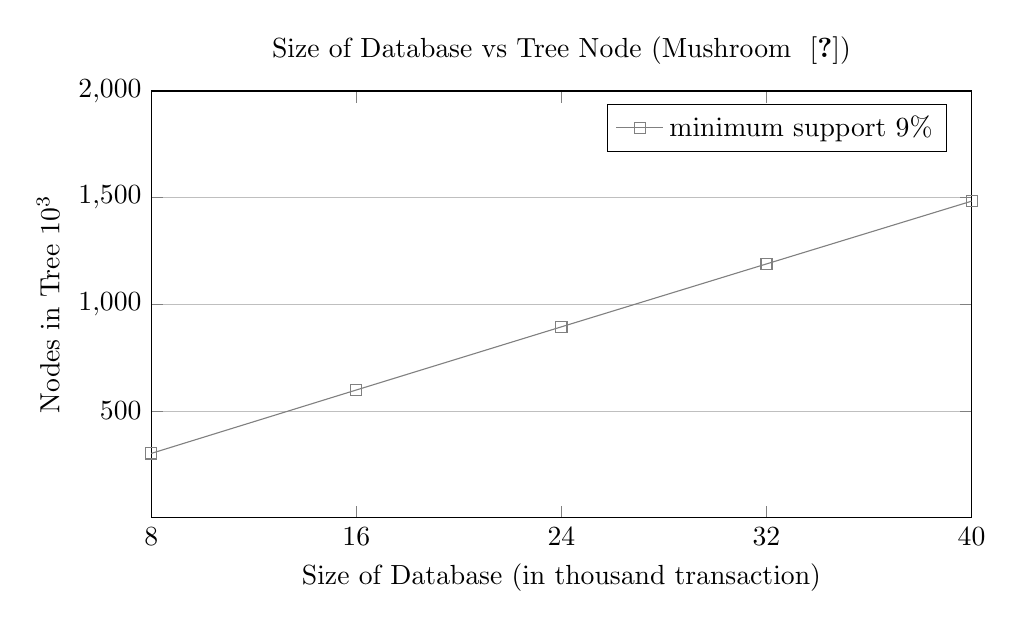
\begin{tikzpicture}
\begin{axis}[
	title={Size of Database vs Tree Node (Mushroom ~\cite{dataset})},
	width=12cm,
	height=7cm,
    xlabel={Size of Database (in thousand transaction)},
    ylabel={Nodes in Tree $10^3$},
    xmin=8, xmax=40,
    ymin=0, ymax=2000,
    xtick={8,16,24,32,40},
    ytick={500,1000,1500,2000},
    legend pos=north east,
    ymajorgrids=true,
    grid style={line width=.2pt,draw=gray!50},
]
 
\addplot[
    solid,color=gray, every mark/.append style={solid, fill=gray}, mark=square
    ]
    coordinates {
			(8,300.856)
			(16,598.221)
			(24,894.225)
			(32,1189.166)
			(40,1483.378)



	};
    \addlegendentry{minimum support 9\%}

\end{axis}
\end{tikzpicture}
%\end{document}
		\caption{Size of Database vs Total Nodes in Tree for T40I10D100K Dataset ~\cite{dataset}}
		\label{result:g_t10_const_tran_mem}
		\end{figure}

	\paragraph{Window Size Change Effect}For window size change effect we have experiment our algorithm in different angle. Experiment shows the window size change effect do not hamper performance and it is consistent. Figure \ref{result:g_m_const_batch} and figure \ref{result:g_t10_const_batch} shows effect of window size change effect on mushroom and T40I10D100K dataset.
		%%%%%%%%%%%%%%%%%%%%%%%%%%%%%%%%%%%%%%%%%%%%%%%%%%%%%%%%%%%%%%%%%%%%%%%%%%%%%%%%%%%%%%%%%%%%%%%%%%%%%%%%%%%%%%%%%%%%%%%%%%%%%%%%%%%%%%%%%%%%%%%%%%%%%%%%%%%%%%%%%%%%%%%%%%%%%%%%%%%%%%%%%%%%%%%%%%%%%%%%%%%%%%%%%%%%%%%%%%%%%
		\begin{figure}[h]
		\centering
			%mark = star, diamond, square, otimes
%\documentclass{article}
%\usepackage{pgfplots}
%\usepackage[justification=centering]{caption}
%\pgfplotsset{compat=newest}
%\begin{document}
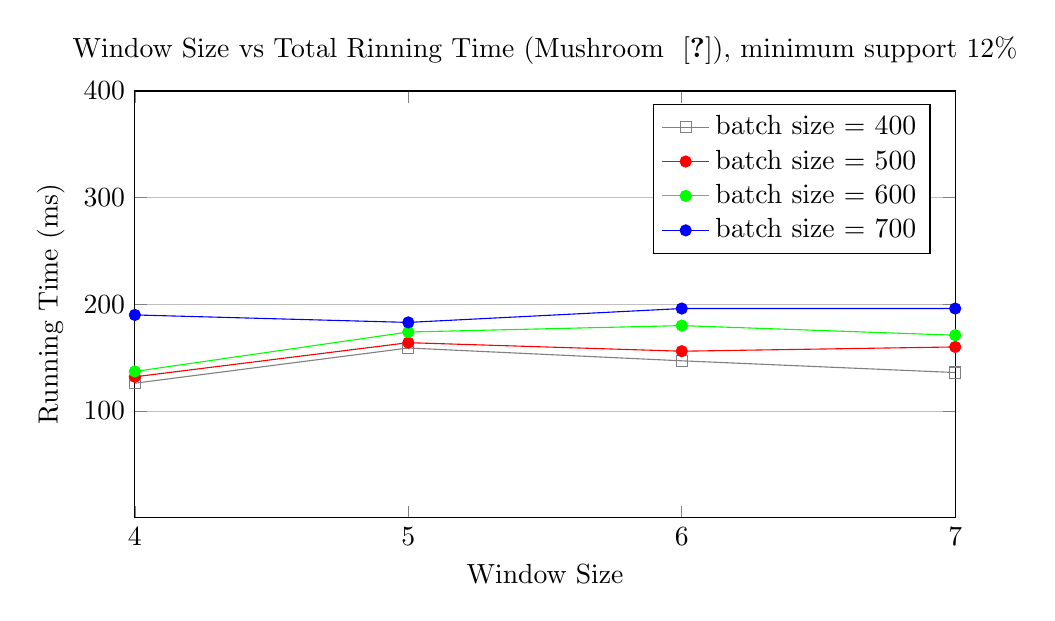
\begin{tikzpicture}
\begin{axis}[
 title={Window Size vs Total Rinning Time (Mushroom ~\cite{dataset}), minimum support 12\%},
 width=12cm,
   height=7cm,
    xlabel={Window Size},
	    ylabel={Running Time (ms)},
    xmin=4, xmax=7,
    ymin=0, ymax=400,
    xtick={4,5,6,7},
    ytick={100,200,300,400},
    legend pos=north east,
    ymajorgrids=true,
    grid style={line width=.2pt,draw=gray!50},
]
 
\addplot[
    solid,color=gray, every mark/.append style={solid, fill=gray}, mark=square
    ]
    coordinates {
			(4,126)			
			(5,159)			
			(6,147)			
			(7,136)
	};
    \addlegendentry{batch size $=$ 400}

	\addplot[
    solid,color=red, every mark/.append style={solid, fill=red}, mark=*
    ]
    coordinates {
			(4,132)			
			(5,164)			
			(6,156)			
			(7,160)
};
    \addlegendentry{batch size $=$ 500}
	

\addplot[
    solid,color=green, every mark/.append style={solid, fill=green}, mark=*
    ]
    coordinates {
			(4,137)			
			(5,174)			
			(6,180)			
			(7,171)
};
    \addlegendentry{batch size $=$ 600}
	
	
\addplot[
    solid,color=blue, every mark/.append style={solid, fill=blue}, mark=*
    ]
    coordinates {
			(4,190)			
			(5,183)			
			(6,196)			
			(7,196)
};
    \addlegendentry{batch size = 700}
\end{axis}
\end{tikzpicture}
%\end{document}
		\caption{Batch Size vs Running Time for Mushroom Dataset ~\cite{dataset}}
		\label{result:g_m_const_batch}
		\end{figure}
		\begin{figure}[h]
		\centering
			%mark = star, diamond, square, otimes
%\documentclass{article}
%\usepackage{pgfplots}
%\usepackage[justification=centering]{caption}
%\pgfplotsset{compat=newest}
%\begin{document}
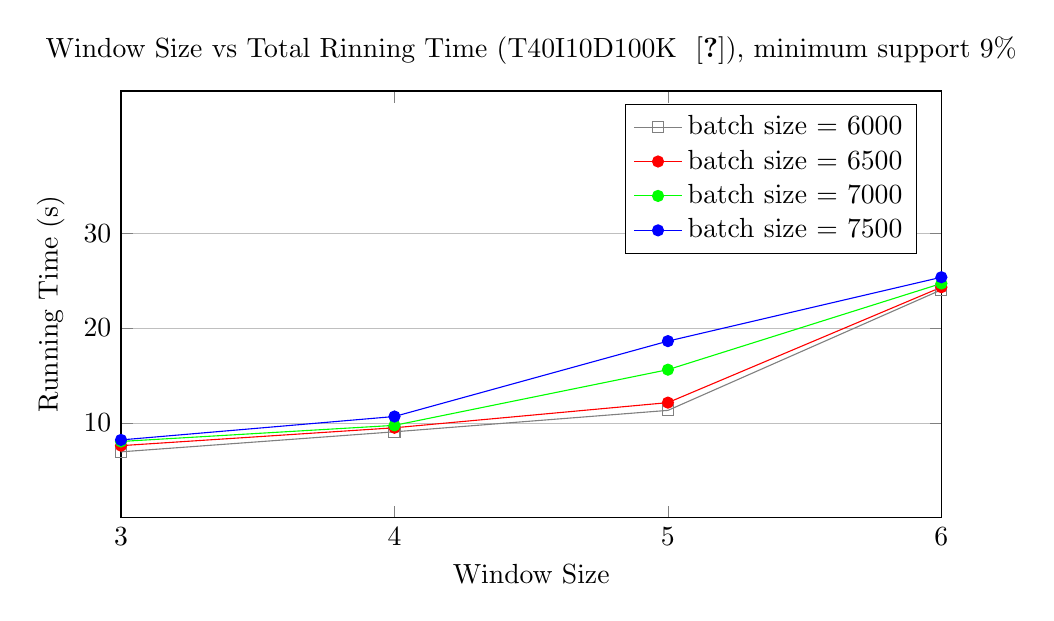
\begin{tikzpicture}
\begin{axis}[
 title={Window Size vs Total Rinning Time (T40I10D100K ~\cite{dataset}), minimum support 9\%},
 width=12cm,
   height=7cm,
    xlabel={Window Size},
    ylabel={Running Time (s)},
    xmin=3, xmax=6,
    ymin=0, ymax=45,
    xtick={3,4,5,6},
    ytick={10,20,30},
    legend pos=north east,
    ymajorgrids=true,
    grid style={line width=.2pt,draw=gray!50},
]
 
\addplot[
    solid,color=gray, every mark/.append style={solid, fill=gray}, mark=square
    ]
    coordinates {
		(3,6.935 )
		(4,9.048 )
		(5,11.308)
		(6,24.026)

	};
    \addlegendentry{batch size $=$ 6000}

	\addplot[
    solid,color=red, every mark/.append style={solid, fill=red}, mark=*
    ]
    coordinates {
		(3,7.587)
		(4,9.473)
		(5,12.126)
		(6,24.299)
};
    \addlegendentry{batch size $=$ 6500}
	

\addplot[
    solid,color=green, every mark/.append style={solid, fill=green}, mark=*
    ]
    coordinates {
		(3,8.030)
		(4,9.729)
		(5,15.602)
		(6,24.690)

};
    \addlegendentry{batch size $=$ 7000}
	
	
\addplot[
    solid,color=blue, every mark/.append style={solid, fill=blue}, mark=*
    ]
    coordinates {
		(3,8.192)
		(4,10.662)
		(5,18.613)
		(6,25.351)
};
    \addlegendentry{batch size $=$ 7500}
\end{axis}
\end{tikzpicture}
%\end{document}
		\caption{Batch Size vs Running Time for T40I10D100K Dataset ~\cite{dataset}}
		\label{result:g_t10_const_batch}
		\end{figure}
		%%%%%%%%%%%%%%%%%%%%%%%%%%%%%%%%%%%%%%%%%%%%%%%%%%%%%%%%%%%%%%%%%%%%%%%%%%%%%%%%%%%%%%%%%%%%%%%%%%%%%%%%%%%%%%%%%%%%%%%%%%%%%%%%%%%%%%%%%%%%%%%%%%%%%%%%%%%%%%%%%%%%%%%%%%%%%%%%%%%%%%%%%%%%%%%%%%%%%%%%%%%%%%%%%%%%%%%		
	\paragraph{Batch Size Change Effect}Like batch change effect we also experimented for batch size change effect.For changing batch size in different volume the result we find is consistent. For constant window and variable batches we have simulated our proposed algorithms. Figure \ref{result:g_m_const_batch} and figure \ref{result:g_t10_const_batch} shows effect of batch size change effect on mushroom and T40I10D100K dataset.
		\begin{figure}[h]
		\centering
			%mark = star, diamond, square, otimes
%\documentclass{article}
%\usepackage{pgfplots}
%\usepackage[justification=centering]{caption}
%\pgfplotsset{compat=newest}
%\begin{document}
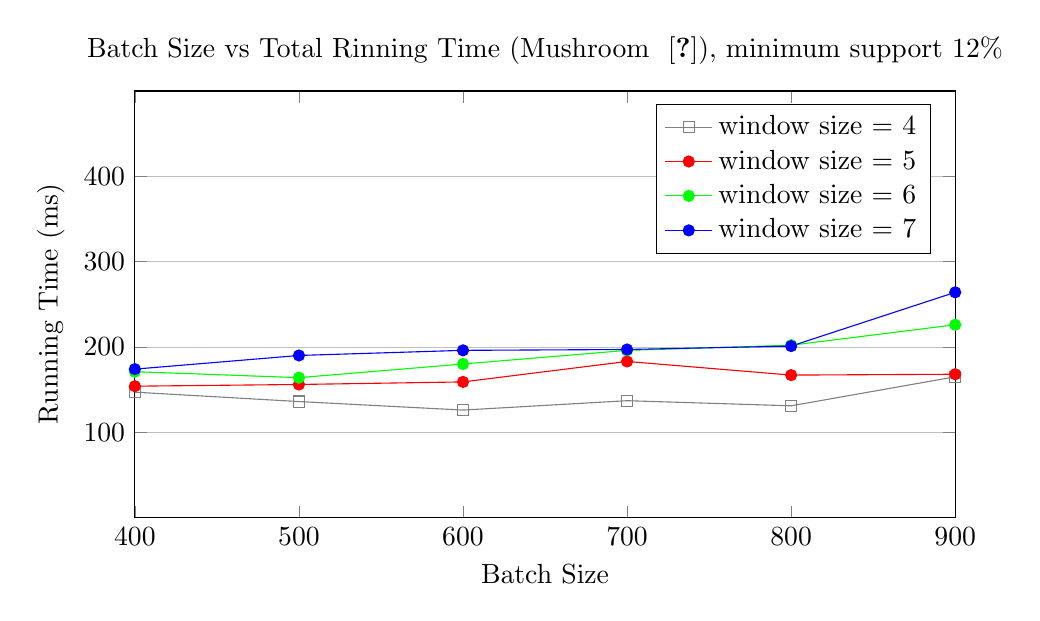
\begin{tikzpicture}
\begin{axis}[
 title={Batch Size vs Total Rinning Time (Mushroom ~\cite{dataset}), minimum support 12\%},
 width=12cm,
   height=7cm,
    xlabel={Batch Size},
    ylabel={Running Time (ms)},
    xmin=400, xmax=900,
    ymin=0, ymax=500,
    xtick={400,500,600,700,800,900},
    ytick={100,200,300,400},
    legend pos=north east,
    ymajorgrids=true,
    grid style={line width=.2pt,draw=gray!50},
]
 
\addplot[
    solid,color=gray, every mark/.append style={solid, fill=gray}, mark=square
    ]
    coordinates {
			(400,147)
			(500,136)
			(600,126)
			(700,137)
			(800,131)
			(900,165)
	};
    \addlegendentry{window size $=$ 4}

	\addplot[
    solid,color=red, every mark/.append style={solid, fill=red}, mark=*
    ]
    coordinates {
			(400,154)
			(500,156)
			(600,159)
			(700,183)
			(800,167)
			(900,168)
};
    \addlegendentry{window size $=$ 5}
	

\addplot[
    solid,color=green, every mark/.append style={solid, fill=green}, mark=*
    ]
    coordinates {
			(400,171)
			(500,164)
			(600,180)
			(700,196)
			(800,202)
			(900,226)
};
    \addlegendentry{window size $=$ 6}
	
	
\addplot[
    solid,color=blue, every mark/.append style={solid, fill=blue}, mark=*
    ]
    coordinates {
			(400,174)
			(500,190)
			(600,196)
			(700,197)
			(800,201)
			(900,264)
};
    \addlegendentry{window size = 7}
\end{axis}
\end{tikzpicture}
%\end{document}
		\caption{Window Size vs Running Time for Mushroom Dataset ~\cite{dataset}}
		\label{result:g_m_const_win}
		\end{figure}
		\begin{figure}[h]
		\centering
			%mark = star, diamond, square, otimes
%\documentclass{article}
%\usepackage{pgfplots}
%\usepackage[justification=centering]{caption}
%\pgfplotsset{compat=newest}
%\begin{document}
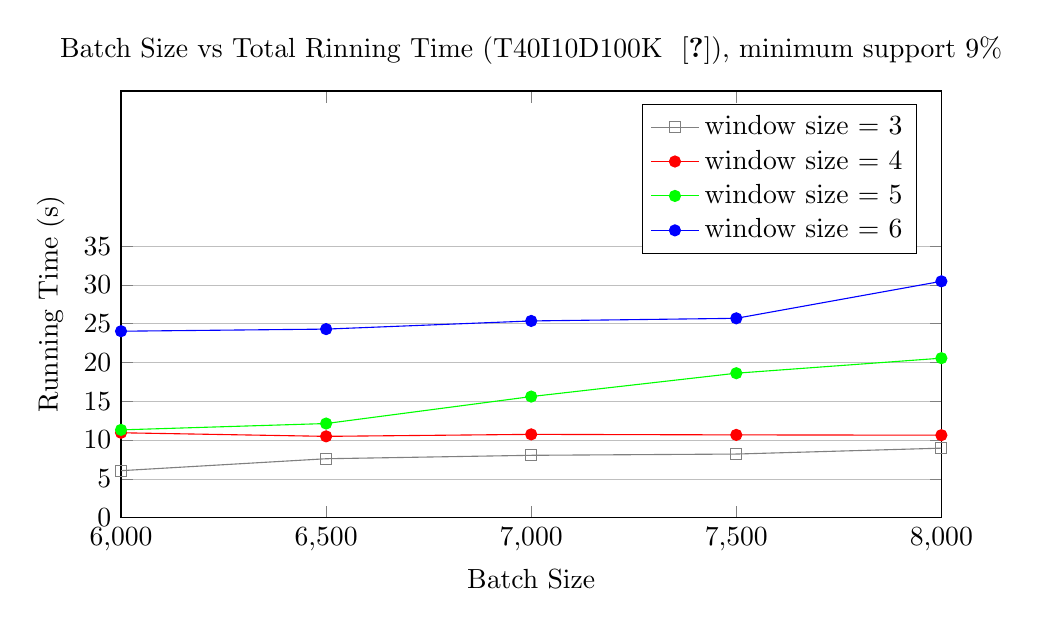
\begin{tikzpicture}
\begin{axis}[
 title={Batch Size vs Total Rinning Time (T40I10D100K ~\cite{dataset}), minimum support 9\%},
 width=12cm,
   height=7cm,
    xlabel={Batch Size},
    ylabel={Running Time (s)},
    xmin=6000, xmax=8000,
    ymin=0, ymax=55,
    xtick={6000,6500,7000,7500,8000},
    ytick={0,5,10,15,20,25,30,35},
    legend pos=north east,
    ymajorgrids=true,
    grid style={line width=.2pt,draw=gray!50},
]
 
\addplot[
    solid,color=gray, every mark/.append style={solid, fill=gray}, mark=square
    ]
    coordinates {
		(6000,6.048)
		(6500,7.587 )
		(7000,8.030 )
		(7500,8.192 )
		(8000,8.951 )
	};
    \addlegendentry{window size $=$ 3}

	\addplot[
    solid,color=red, every mark/.append style={solid, fill=red}, mark=*
    ]
    coordinates {
		(6000,10.935)
		(6500,10.473)
		(7000,10.729)
		(7500,10.662)
		(8000,10.625)

};
    \addlegendentry{window size $=$ 4}
	

\addplot[
    solid,color=green, every mark/.append style={solid, fill=green}, mark=*
    ]
    coordinates {
		(6000,11.308)
		(6500,12.126)
		(7000,15.602)
		(7500,18.613)
		(8000,20.552)

};
    \addlegendentry{window size $=$ 5}
	
	
\addplot[
    solid,color=blue, every mark/.append style={solid, fill=blue}, mark=*
    ]
    coordinates {
		(6000,24.026)
		(6500,24.299)
		(7000,25.351)
		(7500,25.690)
		(8000,30.460)

};
    \addlegendentry{window size $=$ 6}
\end{axis}
\end{tikzpicture}
%\end{document}
		\caption{Window Size vs Running Time for T40I10D100K Dataset ~\cite{dataset}}
		\label{result:g_t10_const_win}
		\end{figure}
		%%%%%%%%%%%%%%%%%%%%%%%%%%%%%%%%%%%%%%%%%%%%%%%%%%%%%%%%%%%%%%%%%%%%%%%%%%%%%%%%%%%%%%%%%%%%%%%%%%%%%%%%%%%%%%%%%%%%%%%%%%%%%%%%%%%%%%%%%%%%%%%%%%%%%%%%%%%%%%%%%%%%%%%%%%%%%%%%%%%%%%%%%%%%%%%%%%%%%%%%%%%%%%%%%%%%%%%%%%%%%
\clearpage
%%%%%%%%%%%%%%%%%%%%%%%%%%%%%%%%%%%%%%%%%%%%%%%%%%%%%%%%%%%%%%%%%%%%%%%%%%%%%%%%%%%%%%%%%%%%%%%%%%%%%%%%%%%%%%%%%%%%%%%%%%%%%%%%%%%%%%%%%%%%%%%%%%%%%%%%%%%%%%%%%%%%%%%%%%%%%%%%%%%%%%%%%%%%%%%%%%%%%%%%%%%%%%%%%%%%%%%%%%%%		
\subsection{Comparison With Existing Approaches}
Here now we have compared our proposed approach with existing system. We have choose SUF-growth ~\cite{suf_growth}  for comparison. This algorithm is perfectly fit for uncertain stream data mining. UF-streaming also designed for mining frequent patterns from uncertain stream but in ~\cite{suf_growth} it has been proved that in all criteria (running time, memory and correctness) SUF-growth ~\cite{suf_growth} is better than UF-streaming ~\cite{suf_growth}. We have experimented for both running time performance and memory efficiency. The result has described below:
	\subsubsection{Running Time Comparison}
	Run time comparison has been experimented and the in the result we found is consistent and we have gained run time efficiency for both dense and sparse dataset. For mushroom dataset our approach's total tree construction time , total mining time and total time has been compared with SUF-growth ~\cite{suf_growth}'s tree construction time and mining time and total time. Figure \ref{result:g_m_tree_construction_total}, figure \ref{result:g_m_mining_total} and figure \ref{result:g_m_total} shows the result graph. As mushroom is a dense database we gain much more in run time. For dense characteristic the constructed \emph{US-tree} is very much compact and more over when mining compact tree the mining time surprisingly decreases that effect the total time. Figure \ref{result:g_t10_tree_construction_total}, figure \ref{result:g_t10_mining_total} and figure \ref{result:g_t10_total} shows same comparison for T40I10D100K dataset ~\cite{dataset}. The graphs shows that our algorithm works correctly for sparse dataset too. Figure \ref{result:g_chess_tree_construction_total}, figure \ref{result:g_chess_mining_total} and figure \ref{result:g_chess_total} shows tree construction time, mining time and total time for chess dataset. This one is dense dataset and the result is consistent, efficient and also scalable.
			\begin{figure}[h]
			\centering
				%%mark = star, diamond, square, otimes
%\documentclass{article}
%\usepackage{pgfplots}
%\usepackage[justification=centering]{caption}
%\pgfplotsset{compat=newest}
%\begin{document}
\begin{figure}
\centering

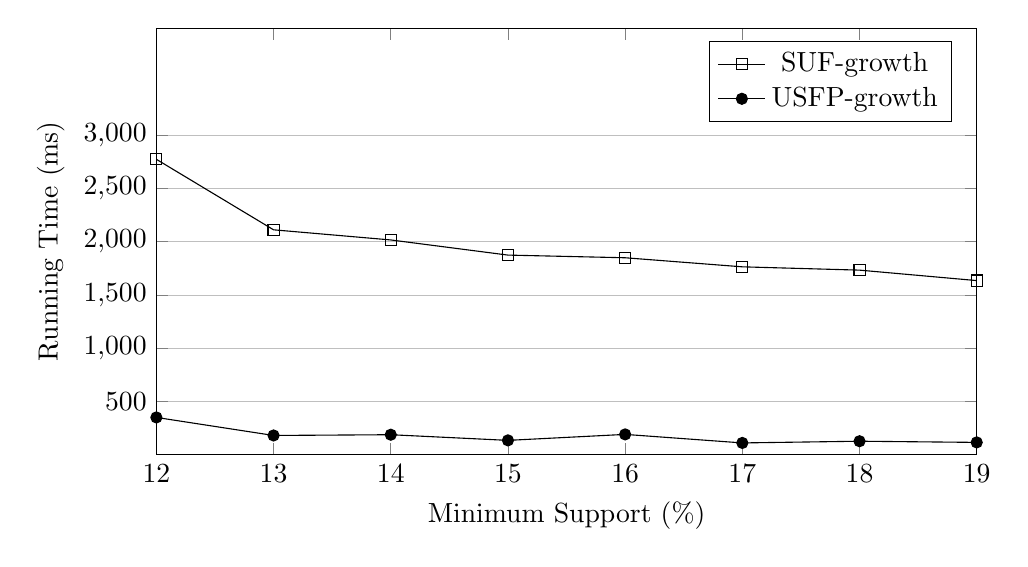
\begin{tikzpicture}
\begin{axis}[
 width=12cm,
   height=7cm,
    xlabel={Minimum Support (\%) },
    ylabel={Running Time (ms)},
    xmin=12, xmax=19,
    ymin=0, ymax=4000,
    xtick={12,13,14,15,16,17,18,19},
    ytick={500,1000,1500,2000,2500,3000},
    legend pos=north east,
    ymajorgrids=true,
    grid style={line width=.2pt,draw=gray!50},
]
 
\addplot[
    solid, every mark/.append style={solid, fill=gray}, mark=square
    ]
    coordinates {
	(12,2771)
	(13,2110)
	(14,2015)
	(15,1873)
	(16,1848)
	(17,1763)
	(18,1732)
	(19,1634)
	};
    \addlegendentry{SUF-growth}
\addplot[
    solid, every mark/.append style={solid, fill=black}, mark=*
    ]
    coordinates {
	(12,351)
	(13,182)
	(14,189)
	(15,136)
	(16,192)
	(17,112)
	(18,128)
	(19,117)
};
    \addlegendentry{USFP-growth}
 
\end{axis}
\end{tikzpicture}
%\caption{Total Tree Construction Time vs Minimum Suppport (\%) \\(Window Size = 4, Frame Size = 650) for mushroom database}
\label{result:mushroom_tree_total}
\end{figure}
%\end{document}
			\caption{Total Tree Construction Time vs Minimum Support (\%) for Mushroom Dataset ~\cite{dataset}}
			\label{result:g_m_tree_construction_total}
			\end{figure}
			
			\begin{figure}[h]
			\centering
				%mark = star, diamond, square, otimes
\documentclass{article}
\usepackage{pgfplots}
\usepackage[justification=centering]{caption}
\pgfplotsset{compat=newest}
\begin{document}
\begin{figure}
\centering

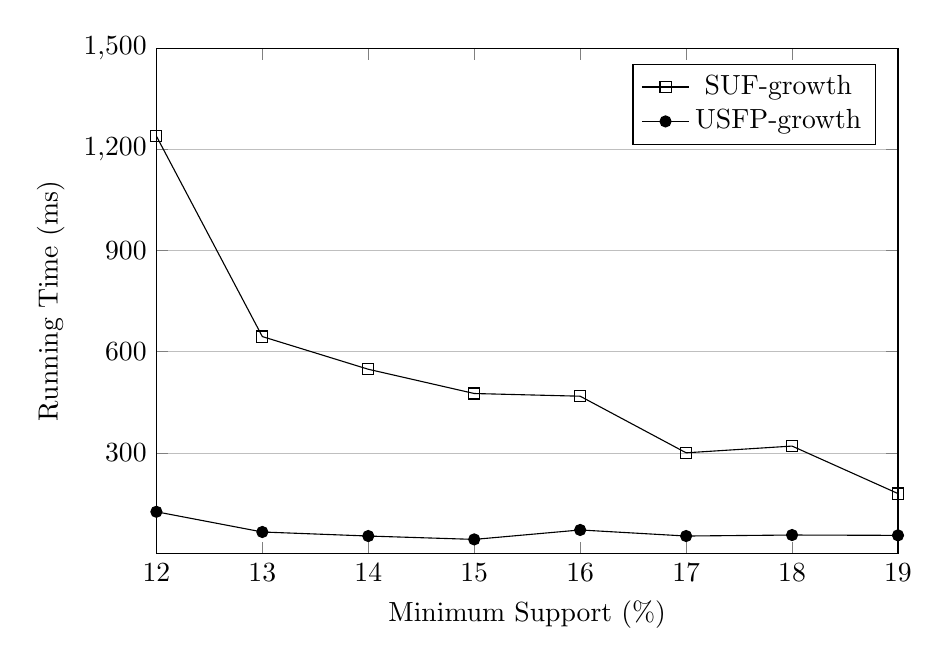
\begin{tikzpicture}
\begin{axis}[
 width=11cm,
   height=8cm,
    xlabel={Minimum Support (\%) },
    ylabel={Running Time (ms)},
    xmin=12, xmax=19,
    ymin=0, ymax=1500,
    xtick={12,13,14,15,16,17,18,19},
    ytick={300,600,900,1200,1500,2000},
    legend pos=north east,
    ymajorgrids=true,
    grid style={line width=.2pt,draw=gray!50},
]
 
\addplot[
    solid, every mark/.append style={solid, fill=gray}, mark=square
    ]
    coordinates {
	(12,1240)
	(13,645)
	(14,548)
	(15,476)
	(16,468)
	(17,300)
	(18,320)
	(19,179)
};
    \addlegendentry{SUF-growth}
\addplot[
    solid, every mark/.append style={solid, fill=black}, mark=*
    ]
    coordinates {
	(12,125)
	(13,65 )
	(14,53 )
	(15,43 )
	(16,71 )
	(17,53 )
	(18,56 )
	(19,55 )
};
    \addlegendentry{USFP-growth}
 
\end{axis}
\end{tikzpicture}
\caption{Total Tree Mining vs Minimum Suppport (\%) \\(Window Size = 4, Frame Size = 650) for mushroom database}
\label{result:mushroom_total}
\end{figure}
\end{document}
			\caption{Total Tree Mining Time vs Minimum Support (\%) for Mushroom Dataset ~\cite{dataset}}
			\label{result:g_m_mining_total}
			\end{figure}
			\begin{figure}[h]
			\centering
				%%mark = star, diamond, square, otimes
%\documentclass{article}
%\usepackage{pgfplots}
%\usepackage[justification=centering]{caption}
%\pgfplotsset{compat=newest}
%\begin{document}
\begin{figure}
\centering

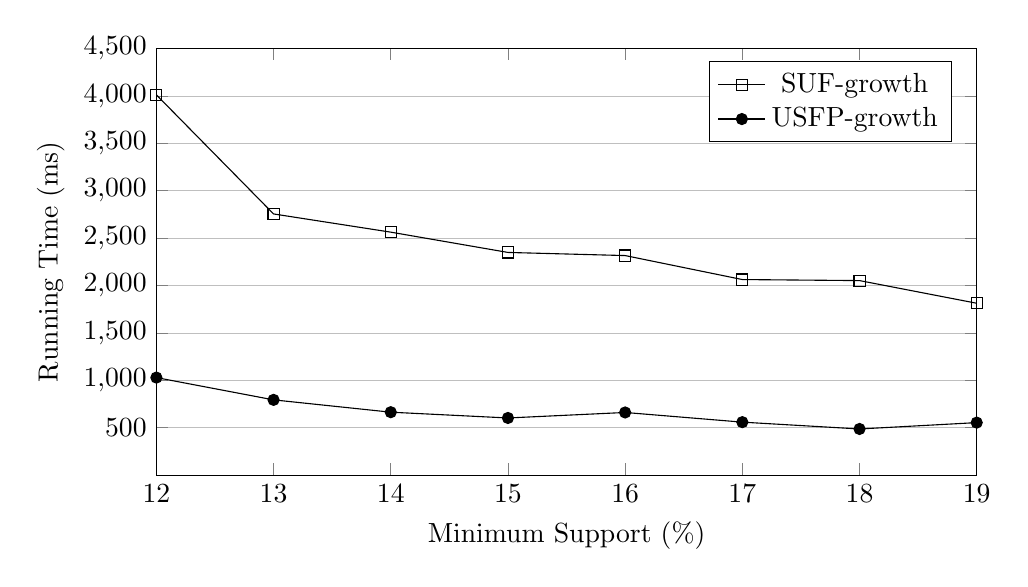
\begin{tikzpicture}
\begin{axis}[
 width=12cm,
   height=7cm,
    xlabel={Minimum Support (\%) },
    ylabel={Running Time (ms)},
    xmin=12, xmax=19,
    ymin=0, ymax=4500,
    xtick={12,13,14,15,16,17,18,19},
    ytick={500,1000,1500,2000,2500,3000,3500,4000,4500},
    legend pos=north east,
    ymajorgrids=true,
    grid style={line width=.2pt,draw=gray!50},
]
 
\addplot[
    solid, every mark/.append style={solid, fill=gray}, mark=square
    ]
    coordinates {
	(12,4011)
	(13,2755)
	(14,2563)
	(15,2349)
	(16,2316)
	(17,2063)
	(18,2052)
	(19,1813)
};
    \addlegendentry{SUF-growth}
\addplot[
    solid, every mark/.append style={solid, fill=black}, mark=*
    ]
    coordinates {
	(12,1029)
	(13,794)
	(14,664)
	(15,603)
	(16,661)
	(17,559)
	(18,487)
	(19,554)
};
    \addlegendentry{USFP-growth}
 
\end{axis}
\end{tikzpicture}
caption{Total Time (Tree Construction + Mining + False Positive Reduction) vs Minimum Suppport (\%) ( Window Size = 4, Frame Size = 650 ) for mushroom database}
\label{result:mushroom_total}
\end{figure}
%\end{document}
			\caption{Running Time vs Minimum Support (\%) for Mushroom Dataset ~\cite{dataset}}
			\label{result:g_m_total}
			\end{figure}
			\begin{figure}[h]
			\centering
				%%mark = star, diamond, square, otimes
%\documentclass{article}
%\usepackage{pgfplots}
%\usepackage[justification=centering]{caption}
%\pgfplotsset{compat=newest} 	title={\parbox{\linewidth}{\centering Total Tree Construction Time vs Minimum Suppport (\%) for T40I10D100K ~\cite{dataset}, Window Size = 5, Frame Size = 7000}},
%\begin{document}
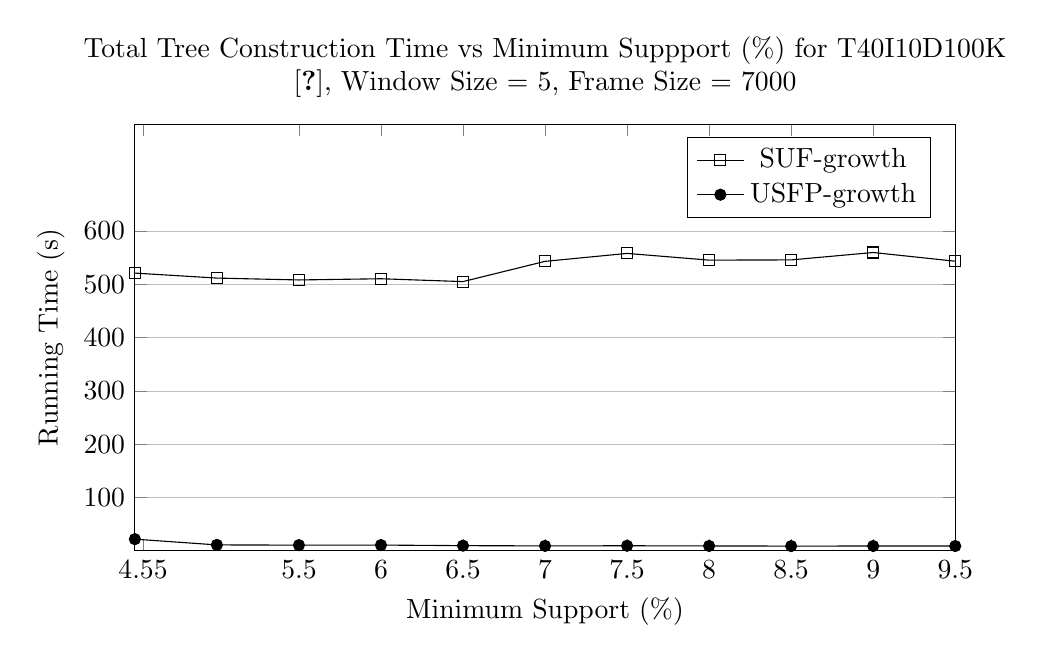
\begin{tikzpicture}
	\begin{axis}[
	title={\parbox{\linewidth}{\centering Total Tree Construction Time vs Minimum Suppport (\%) for T40I10D100K ~\cite{dataset}, Window Size = 5, Frame Size = 7000}},
	width=12cm,
	height=7cm,
    xlabel={Minimum Support (\%) },
    ylabel={Running Time (s)},
    xmin=4.5, xmax=9.5,
    ymin=0, ymax=800,
    xtick={4.55,5.5,6,6.5,7,7.5,8,8.5,9,9.5},
    ytick={100,200,300,400,500,600},
    legend pos=north east,
    ymajorgrids=true,
    grid style={line width=.2pt,draw=gray!50},
]
 
\addplot[
    solid, every mark/.append style={solid, fill=gray}, mark=square
    ]
    coordinates {
			(4.5,520.723)
			(5  ,511.365)
			(5.5,507.854)
			(6  ,510.12 )
			(6.5,504.767)
			(7  ,542.742)
			(7.5,557.633)
			(8  ,545.039)
			(8.5,545.444)
			(9  ,559.335)
			(9.5,542.996)

	};
    \addlegendentry{SUF-growth}
\addplot[
    solid, every mark/.append style={solid, fill=black}, mark=*
    ]
    coordinates {
		(4.5,21.814)
		(5  ,11.035)
		(5.5,10.601)
		(6  ,10.723)
		(6.5,9.646 )
		(7  ,9.177 )
		(7.5,9.427 )
		(8  ,9.092 )
		(8.5,8.8   )
		(9  ,8.95  )
		(9.5,8.883 )

};
    \addlegendentry{USFP-growth}
 
\end{axis}
\end{tikzpicture}
%\end{document}
			\caption{Total Tree Construction Time vs Minimum Support (\%) for T40I10D100K Dataset ~\cite{dataset}}
			\label{result:g_t10_tree_construction_total}
			\end{figure}
			
			\begin{figure}[h]
			\centering
				%%%mark = star, diamond, square, otimes
%\documentclass{article}
%\usepackage{pgfplots}
%\usepackage[justification=centering]{caption}
%\pgfplotsset{compat=newest}
%\begin{document}
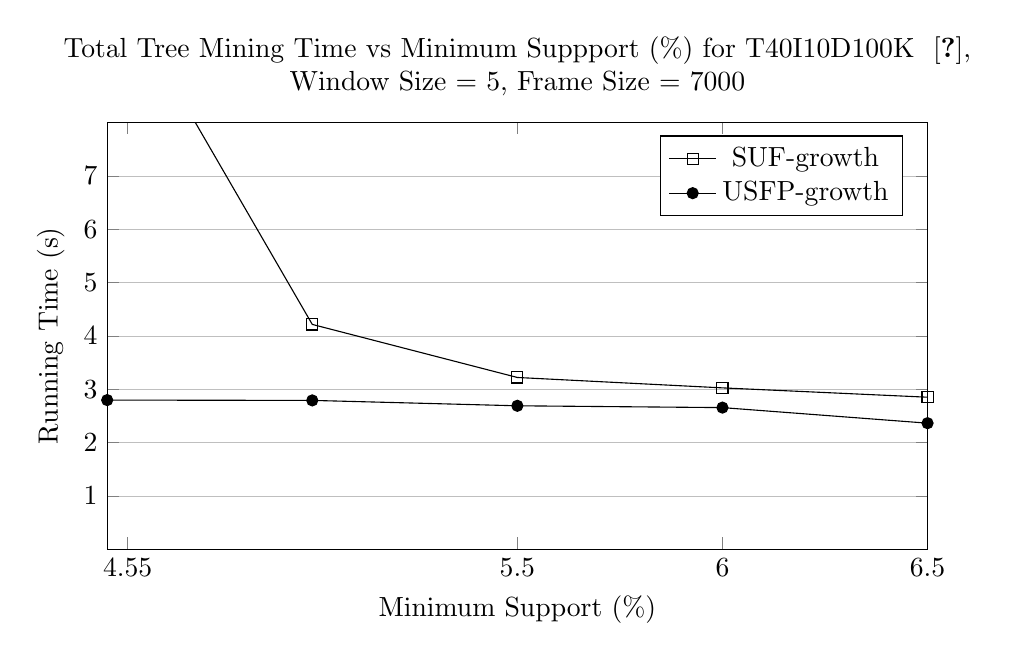
\begin{tikzpicture}
\begin{axis}[
	title={\parbox{\linewidth}{\centering Total Tree Mining Time vs Minimum Suppport (\%) for T40I10D100K ~\cite{dataset}, Window Size = 5, Frame Size = 7000}},
	width=12cm,
	height=7cm,
    xlabel={Minimum Support (\%) },
    ylabel={Running Time (s)},
    xmin=4.5, xmax=6.5,
    ymin=0, ymax=8,
    xtick={4.55,5.5,6,6.5},
    ytick={1,2,3,4,5,6,7},
    legend pos=north east,
    ymajorgrids=true,
    grid style={line width=.2pt,draw=gray!50},
]
 
\addplot[
    solid, every mark/.append style={solid, fill=gray}, mark=square
    ]
    coordinates {
			(4.5,10.856)
			(5  ,4.216 )
			(5.5,3.221 )
			(6  ,3.026 )
			(6.5,2.851 )


};
    \addlegendentry{SUF-growth}
\addplot[
    solid, every mark/.append style={solid, fill=black}, mark=*
    ]
    coordinates {
			(4.5,  2.797)
			(5  , 2.791)
			(5.5,2.69 )
			(6  ,2.656 )
			(6.5,2.364 )


};
    \addlegendentry{USFP-growth}
 
\end{axis}
\end{tikzpicture}
%\end{document}
			\caption{Total Tree Mining Time vs Minimum Support (\%) for T40I10D100K Dataset ~\cite{dataset}}
			\label{result:g_t10_mining_total}
			\end{figure}
			
			\begin{figure}[h]
			\centering
				%%%mark = star, diamond, square, otimes
%\documentclass{article}
%\usepackage{pgfplots}
%\usepackage[justification=centering]{caption}
%\pgfplotsset{compat=newest}
%\begin{document}
\begin{figure}[!h]
\centering

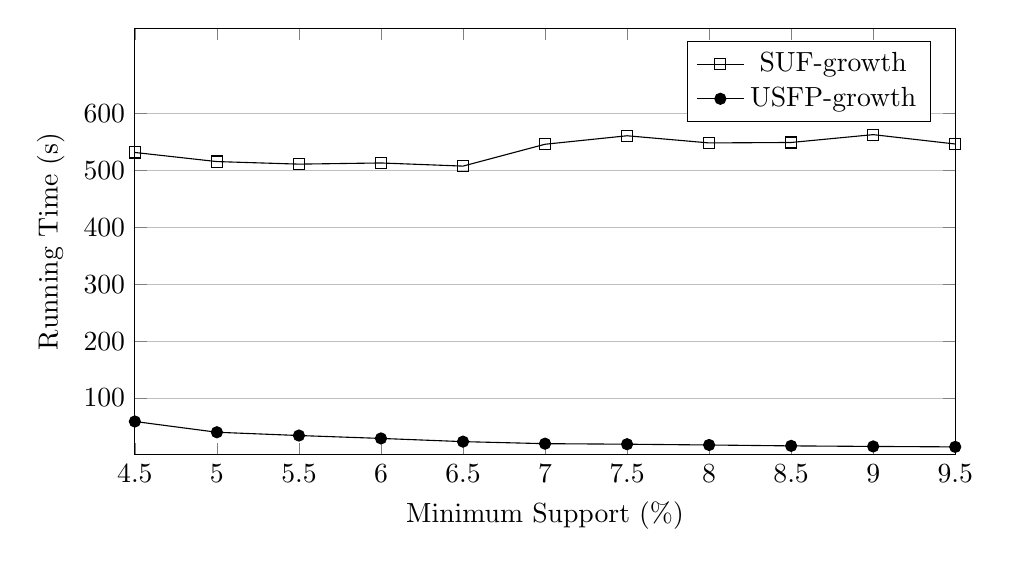
\begin{tikzpicture}
\begin{axis}[
 width=12cm,
   height=7cm,
    xlabel={Minimum Support (\%) },
    ylabel={Running Time (s)},
    xmin=4.5, xmax=9.5,
    ymin=0, ymax=750,
    xtick={4.5,5,5.5,6,6.5,7,7.5,8,8.5,9,9.5},
    ytick={100,200,300,400,500,600},
    legend pos=north east,
    ymajorgrids=true,
    grid style={line width=.2pt,draw=gray!50},
]
 
\addplot[
    solid, every mark/.append style={solid, fill=gray}, mark=square
    ]
    coordinates {
			(4.5,531.579)
			(5  ,515.581)
			(5.5,511.075)
			(6  ,513.146)
			(6.5,507.618)
			(7  ,546.032)
			(7.5,560.952)
			(8  ,548.354)
			(8.5,549.139)
			(9  ,562.928)
			(9.5,546.47 )

};
    \addlegendentry{SUF-growth}
\addplot[
    solid, every mark/.append style={solid, fill=black}, mark=*
    ]
    coordinates {
			(4.5,58.652)
			(5  ,39.735)
			(5.5,33.993)
			(6  ,28.892)
			(6.5,23.262)
			(7  ,19.669)
			(7.5,18.735)
			(8  ,17.355)
			(8.5,15.785)
			(9  ,14.803)
			(9.5,14.013)

};
    \addlegendentry{USFP-growth}
 
\end{axis}
\end{tikzpicture}
\caption{Total Time (Tree Construction + Mining + False Positive Reduction) vs Minimum Suppport (\%) \\(Window Size = 5, Frame Size = 7000) for T40I10D100K database}
\label{result:t10_total}
\end{figure}
%\end{document}
			\caption{Running Time vs Minimum Support (\%) for T40I10D100K Dataset ~\cite{dataset}}
			\label{result:g_t10_total}
			\end{figure}
	
			\begin{figure}[h]
			\centering
				%%mark = star, diamond, square, otimes
%\documentclass{article}
%\usepackage{pgfplots}
%\usepackage[justification=centering]{caption}
%\pgfplotsset{compat=newest}
%\begin{document} 
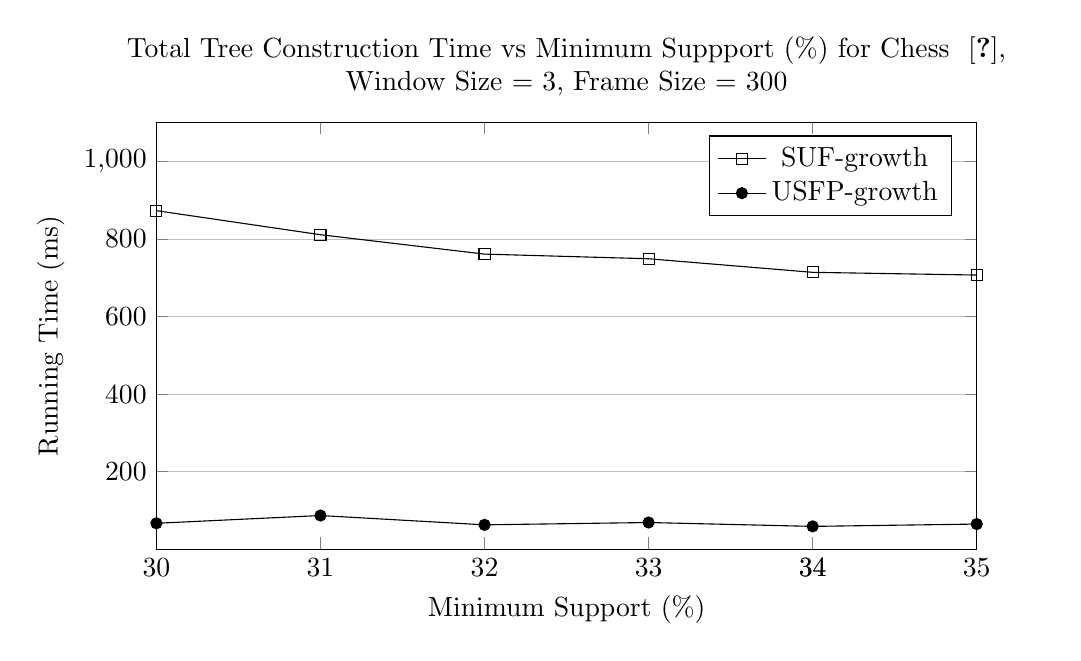
\begin{tikzpicture}
\begin{axis}[
	title={\parbox{\linewidth}{\centering Total Tree Construction Time vs Minimum Suppport (\%) for Chess ~\cite{dataset}, Window Size = 3, Frame Size = 300}},
	width=12cm,
	height=7cm,
    xlabel={Minimum Support (\%) },
    ylabel={Running Time (ms)},
    xmin=30, xmax=35,
    ymin=0, ymax=1100,
    xtick={30,31,32,33,34,34,35},
    ytick={200,400,600,800,1000},
    legend pos=north east,
    ymajorgrids=true,
    grid style={line width=.2pt,draw=gray!50},
]
 
\addplot[
    solid, every mark/.append style={solid, fill=gray}, mark=square
    ]
    coordinates {
			(30,873)
			(31,811)
			(32,761)
			(33,749)
			(34,714)
			(35,707)

	};
    \addlegendentry{SUF-growth}
\addplot[
    solid, every mark/.append style={solid, fill=black}, mark=*
    ]
    coordinates {
			(30,67)
			(31,87)
			(32,63)
			(33,69)
			(34,59)
			(35,65)

};
    \addlegendentry{USFP-growth}
 
\end{axis}
\end{tikzpicture}
%\end{document}
			\caption{Total Tree Construction Time vs Minimum Support (\%) for Chess Dataset ~\cite{dataset}}
			\label{result:g_chess_tree_construction_total}
			\end{figure}
			
			\begin{figure}[h]
			\centering
				%%mark = star, diamond, square, otimes
%\documentclass{article}
%\usepackage{pgfplots}
%\usepackage[justification=centering]{caption}
%\pgfplotsset{compat=newest}
%\begin{document}
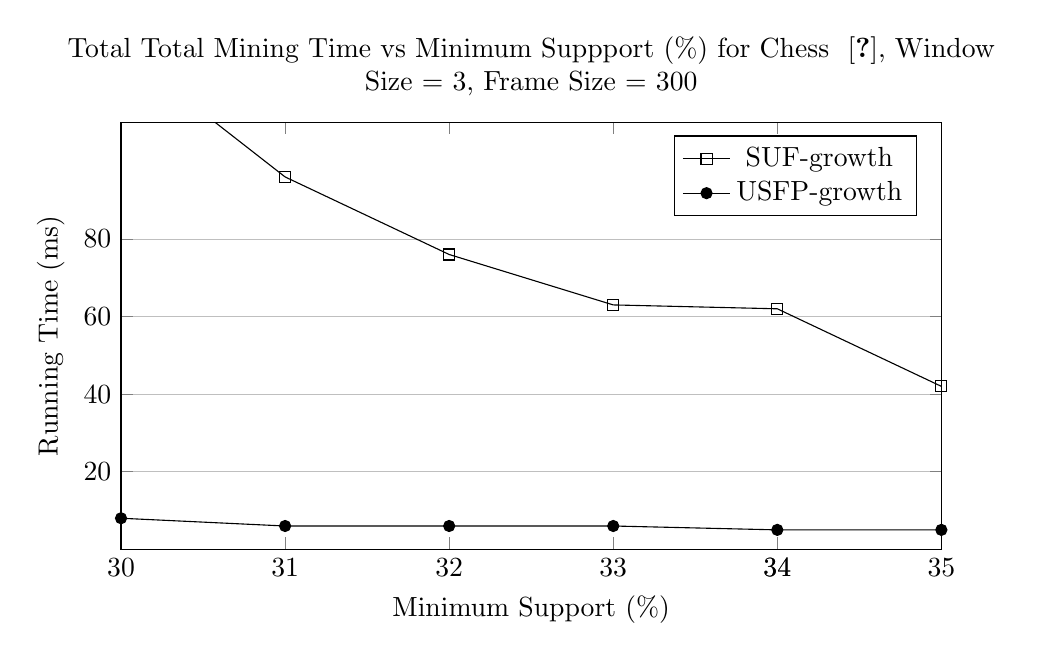
\begin{tikzpicture}
\begin{axis}[
	title={\parbox{\linewidth}{\centering Total Total Mining Time vs Minimum Suppport (\%) for Chess ~\cite{dataset}, Window Size = 3, Frame Size = 300}},
	width=12cm,
	height=7cm,
    xlabel={Minimum Support (\%) },
    ylabel={Running Time (ms)},
    xmin=30, xmax=35,
    ymin=0, ymax=110,
    xtick={30,31,32,33,34,34,35},
    ytick={20,40,60,80},
    legend pos=north east,
    ymajorgrids=true,
    grid style={line width=.2pt,draw=gray!50},
]
 
\addplot[
    solid, every mark/.append style={solid, fill=gray}, mark=square
    ]
    coordinates {
			(30,129)
			(31,96)
			(32,76)
			(33,63)
			(34,62)
			(35,42)

};
    \addlegendentry{SUF-growth}
\addplot[
    solid, every mark/.append style={solid, fill=black}, mark=*
    ]
    coordinates {
			(30,8)
			(31,6)
			(32,6)
			(33,6)
			(34,5)
			(35,5)

};
    \addlegendentry{USFP-growth}
 
\end{axis}
\end{tikzpicture}
%\end{document}
			\caption{Total Tree Mining Time vs Minimum Support (\%) for Chess Dataset ~\cite{dataset}}
			\label{result:g_chess_mining_total}
			\end{figure}
			
			\begin{figure}[h]
			\centering
				%%mark = star, diamond, square, otimes
%\documentclass{article}
%\usepackage{pgfplots}
%\usepackage[justification=centering]{caption}
%\pgfplotsset{compat=newest}
%\begin{document}
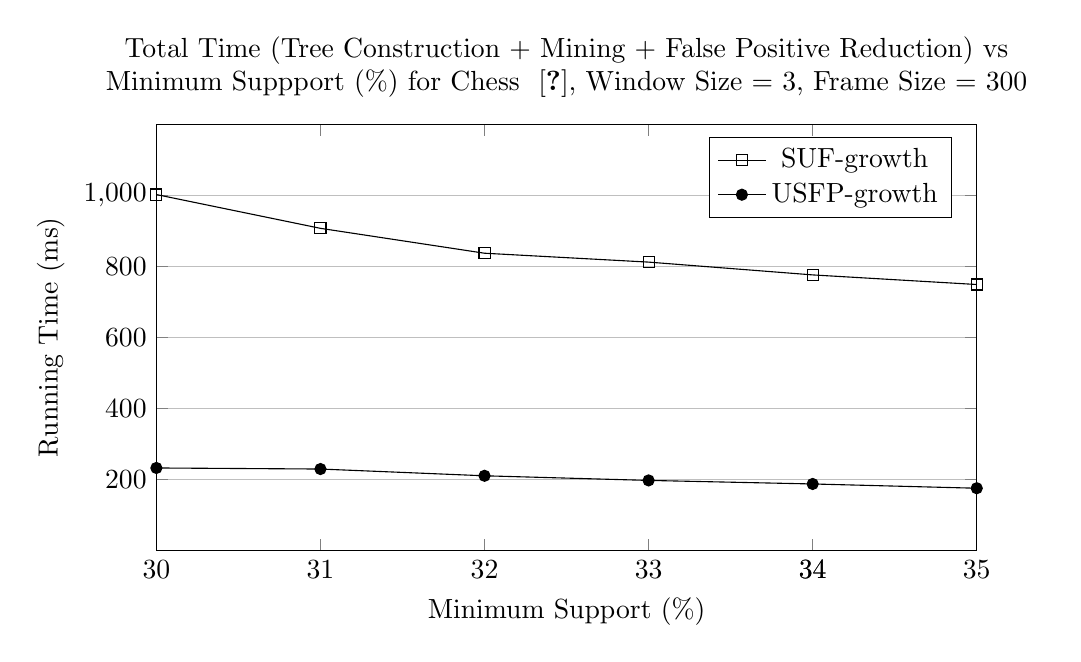
\begin{tikzpicture}
\begin{axis}[
	title={\parbox{\linewidth}{\centering Total Time (Tree Construction + Mining + False Positive Reduction) vs Minimum Suppport (\%) for Chess ~\cite{dataset}, Window Size = 3, Frame Size = 300}},
	width=12cm,
	height=7cm,
    xlabel={Minimum Support (\%) },
    ylabel={Running Time (ms)},
    xmin=30, xmax=35,
    ymin=0, ymax=1200,
    xtick={30,31,32,33,34,34,35},
    ytick={200,400,600,800,1000},
    legend pos=north east,
    ymajorgrids=true,
    grid style={line width=.2pt,draw=gray!50},
]
 
\addplot[
    solid, every mark/.append style={solid, fill=gray}, mark=square
    ]
    coordinates {
			(30,1002)
			(31,907)
			(32,837)
			(33,812)
			(34,776)
			(35,749)
};
    \addlegendentry{SUF-growth}
\addplot[
    solid, every mark/.append style={solid, fill=black}, mark=*
    ]
    coordinates {
			(30,233)
			(31,230)
			(32,211)
			(33,198)
			(34,188)
			(35,176)

};
    \addlegendentry{USFP-growth}
 
\end{axis}
\end{tikzpicture}
%\end{document}
			\caption{Running Time vs Minimum Support (\%) for Chess Dataset ~\cite{dataset}}
			\label{result:g_chess_total}
			\end{figure}
\clearpage
	\subsubsection{Memory Comparison}
		As our proposed \emph{US-tree} have capability to share nodes more than \emph{SUF-growth} ~\cite{dataset}, we get much more gain in memory. The experimental result also indicates that very clearly. Figure \ref{result:g_m_memory_node} shows the memory comparison on mushroom dataset. Mushroom is dense database so we get  much more gain in memory. The graph clearly shows that with the increase of total transaction in the tree gives the much more gain. For chess dataset the the compactness of tree is also very impressive as this dataset is also compact (figure \ref{result:g_chess_memory_node}) the Dense dataset have more scope to share nodes more. Figure \ref{result:g_t10_memory_node} also shows that in T40I10D100K database we also gain the memory optimization. As the database is sparse, we get the memory gain less then dense one.
			\begin{figure}[h]
			\centering
				%mark = star, diamond, square, otimes
%\documentclass{article}
%\usepackage{pgfplots}
%\usepackage[justification=centering]{caption}
%\pgfplotsset{compat=newest}
%\begin{document}
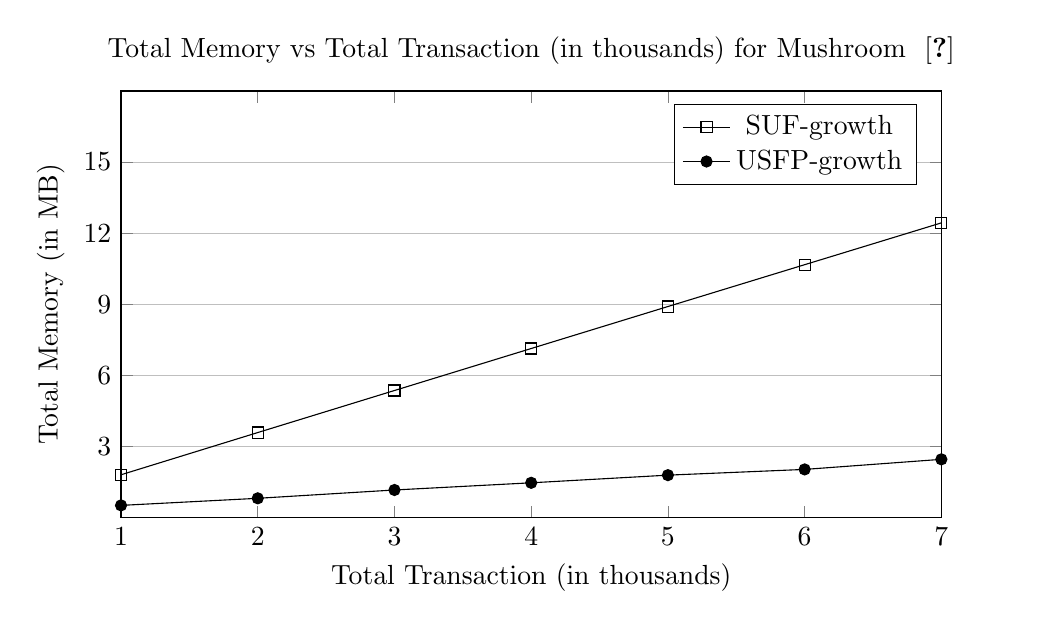
\begin{tikzpicture}
\begin{axis}[
	title={\parbox{\linewidth}{\centering Total Memory vs Total Transaction (in thousands) for Mushroom ~\cite{dataset}}},
	width=12cm,
	height=7cm,
    xlabel={Total Transaction (in thousands) },
    ylabel={Total Memory (in MB) },
    xmin=1, xmax=7,
    ymin=0, ymax=18,
    xtick={1,2,3,4,5,6,7},
    ytick={3,6,9,12,15},
    legend pos=north east,
    ymajorgrids=true,
    grid style={line width=.2pt,draw=gray!50},
]
 
\addplot[
    solid, every mark/.append style={solid, fill=gray}, mark=square
    ]
    coordinates {
			(1,1.807  )
			(2,3.588  )
			(3,5.362  )
			(4,7.134     )
			(5,8.905  )
			(6,10.670 )
			(7,12.434  )



	};
    \addlegendentry{SUF-growth}
\addplot[
    solid, every mark/.append style={solid, fill=black}, mark=*
    ]
    coordinates {
			(1,.5152  )
			(2,.814  )
			(3,1.165 )
			(4,1.468 )
			(5,1.791  )
			(6,2.033 )
			(7,2.458 )


};
    \addlegendentry{USFP-growth}
 
\end{axis}
\end{tikzpicture}
%\end{document}
			\caption{Avg Tree Node per window vs Frame Size for Mushroom Dataset ~\cite{dataset}}
			\label{result:g_m_memory_node}
			\end{figure}
			
			\begin{figure}[h]
			\centering
				%mark = star, diamond, square, otimes
%\documentclass{article}
%\usepackage{pgfplots}
%\usepackage[justification=centering]{caption}
%\pgfplotsset{compat=newest}
%\begin{document}
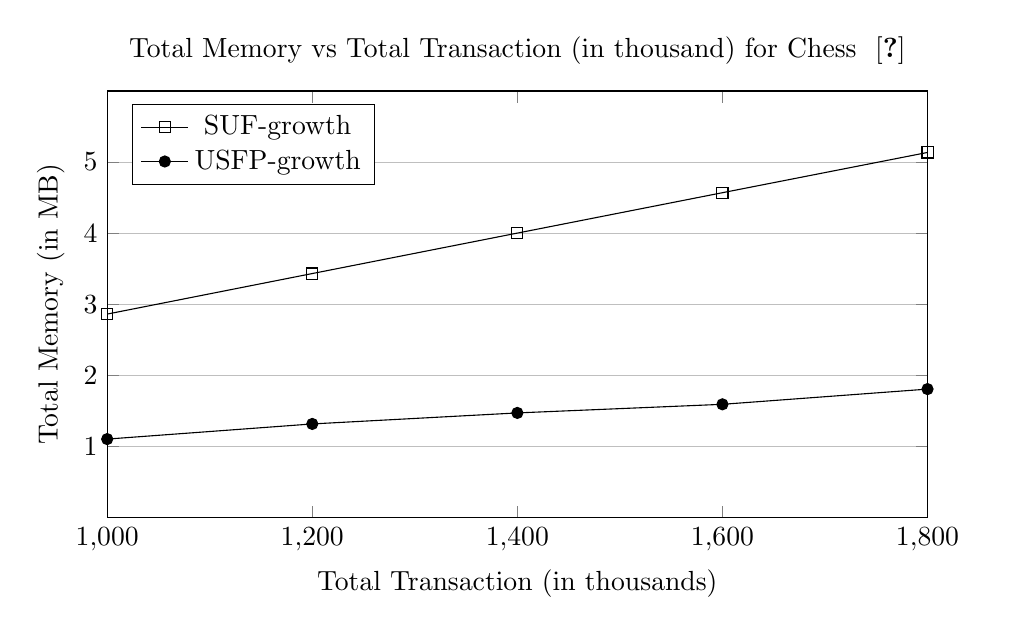
\begin{tikzpicture}
\begin{axis}[
	title={\parbox{\linewidth}{\centering Total Memory vs Total Transaction (in thousand) for Chess ~\cite{dataset}}},
	width=12cm,
	height=7cm,
    xlabel={Total Transaction (in thousands) },
    ylabel={Total Memory (in MB) },
    xmin=1000, xmax=1800,
    ymin=0, ymax=6,
    xtick={600,800,1000,1200,1400,1600,1800},
    ytick={1,2,3,4,5},
    legend pos=north west,
    ymajorgrids=true,
    grid style={line width=.2pt,draw=gray!50},
]
 
\addplot[
    solid, every mark/.append style={solid, fill=gray}, mark=square
    ]
    coordinates {
			(600,	1.720)
			(800,	2.291)
			(1000,	2.862)
			(1200,	3.432)
			(1400,	4.001)
			(1600,	4.569)
            (1800,	5.135)



	};
    \addlegendentry{SUF-growth}
\addplot[
    solid, every mark/.append style={solid, fill=black}, mark=*
    ]
    coordinates {
			(600,	0.681 )
			(800,	0.865 )
			(1000,	1.104 )
			(1200,	1.317 )
			(1400,	1.472 )
			(1600,	1.593 )
            (1800,	1.807 )


};
    \addlegendentry{USFP-growth}
 
\end{axis}
\end{tikzpicture}
%\end{document}
			\caption{Avg Tree Node per window vs Frame Size for Chess Dataset ~\cite{dataset}}
			\label{result:g_chess_memory_node}
			\end{figure}
			
			\begin{figure}[h]
				%%%mark = star, diamond, square, otimes
%\documentclass{article}
%\usepackage{pgfplots}
%\usepackage[justification=centering]{caption}
%\pgfplotsset{compat=newest}
%\begin{document}
\begin{figure}
\centering

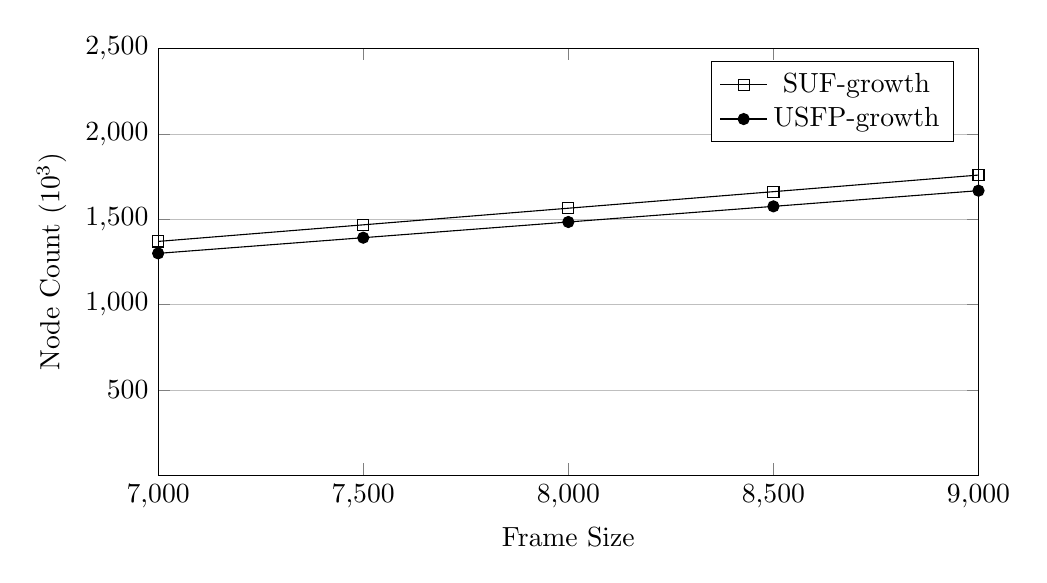
\begin{tikzpicture}
\begin{axis}[
 width=12cm,
   height=7cm,
    xlabel={Frame Size },
    ylabel={Node Count ($10^3$)},
    xmin=7000, xmax=9000,
    ymin=0, ymax=2500,
    xtick={7000,7500,8000,8500,9000},
    ytick={500,1000,1500,2000,2500},
    legend pos=north east,
    ymajorgrids=true,
    grid style={line width=.2pt,draw=gray!50},
]
 
\addplot[
    solid, every mark/.append style={solid, fill=gray}, mark=square
    ]
    coordinates {
			(7000,1369.555 )
			(7500,1466.766 )
			(8000,1564.122 )
			(8500,1661.100 )
			(9000,1758.412 )
			(9500,1855.734 )

	};
    \addlegendentry{SUF-growth}
\addplot[
    solid, every mark/.append style={solid, fill=black}, mark=*
    ]
    coordinates {
					(7000,1299.510)
		(7500,1391.388)
		(8000,1483.378)
		(8500,1574.984)
		(9000,1666.912)
		(9500,1758.773)

};
    \addlegendentry{USFP-growth}
 
\end{axis}
\end{tikzpicture}
\caption{Total Tree Node vs Frame Size (Window Size = 5) for T40I10D100K database}
\label{result:t10_total_mem_node}
\end{figure}
%\end{document}
			\caption{Avg Tree Node per window vs Frame Size for T40I10D100K Dataset ~\cite{dataset}}
			\label{result:g_t10_memory_node}
			\end{figure}
		

\clearpage
\section{Summary}
In summary, our proposed \emph{US-tree}, construction \emph{USFP-growth} mining algorithm is very correct, efficient, scalable algorithm that works fine in any configuration (minimum support, window size, batch size). For dense dataset (both real and synthetic) this is very efficient. For sparse dataset this also gives us gain both in memory and in running time. The \emph{U\textsuperscript{cap}} value gives much more benefit to share nodes in the \emph{US-tree}. The compactness of \emph{US-tree} is surprisingly noticeable. Mining compact \emph{US-tree} gives the main surprise in the running time. The \emph{USFP-growth} mining algorithm works nicely without generating no false negatives and a little amount of false positives that can efficiently be removed using the false positive reduction technique.
%
%\end{document} % Performance Evaluation
%%%
\chapter{Conclusions}
\lhead{Chapter 5. \emph{Conclusions}}
\section{Research Summary}
In this thesis, we have proposed new window-batch based probabilistic strategy for finding frequent patterns from uncertain dynamic data. We have proposed \emph{U\textsuperscript{cap}}, which is the upper bound of existential probability. We have proposed new \emph{US-tree} data-structure that is very compact. For mining, we have proposed \emph{USFP-growth} algorithm that will efficiently and recursively mine frequent patterns from \emph{US-tree}.\\
\\
For calculating \emph{U\textsuperscript{cap}} value we have taken upper-bound of existential probability that makes the node sharing possible between same items. For uncertainty property of data node sharing was very much irregular in existing approaches. In our strategy, this sharingis allowed and that makes the tree more compact and efficient. Our proposed \emph{US-tree} is very compact for possible node sharing much more than existing tree structures (e.g. \emph{SUF-growth} ~\cite{suf_growth}). To handle the stream of data we have proposed to divide the whole transactions into batches and windows that is completely dependent on the system user how much recent data she/he wants to store in the tree. Instead of keeping the support we have kept new meta-information based on \emph{U\textsuperscript{cap}} value that helps further mining. We have developed new algorithm \emph{USFP-growth} mining algorithm that efficiently remove unnecessary patterns from the tree earlier, which helps to gain running time efficiency. Conditional candidate tree needed to be mined in our approach will be less than other approaches. This makes the mining algorithm very much faster. We have also introduced an efficient strategy to remove the false positives generated by our algorithm. Our comprehensive result study shows that total time (tree construction, tree mining, and false positive reduction) is less than existing approaches (e.g. \emph{SUF-growth} ~\cite{suf_growth}). We also developed a frequent pattern tree which may later be used to mine closed patterns and maximal patterns.
\section{Limitations and Scope of Future Studies}
As the frequent pattern mining over the domain of uncertain stream data is a very new, there are some scopes to extend and use our proposed approach as a tool for further research.\\ 
\textbf{Firstly,} we have introduced probabilistic model for calculating \emph{U\textsuperscript{cap}} value. This value can be studied and updated to find both upper and lower bound of existential probability.\\
\textbf{Secondly,} as data-set we worked on, is the stream, which is dynamic it can change dynamically. Once an item comes to the top of the \emph{US-tree} stays there at least it becomes oldest data although may be very much infrequent in the recent data. This case may make the tree not compact that was possible. As data stream cannot be read more than once. So no previously assumption can be done to this tree. So some re-construction after new batch inserted into the window will possibly be the one of the major optimization of the tree.
\section{Conclusions}
 % Conclusion



\addtocontents{toc}{\vspace{2em}}  % Add a gap in the Contents, for aesthetics
\backmatter

%% ----------------------------------------------------------------
\label{Bibliography}
\lhead{\emph{Bibliography}}  % Change the left side page header to "Bibliography"
%\bibliographystyle{unsrtnat}  % Use the "unsrtnat" BibTeX style for formatting the Bibliography
\bibliographystyle{plain}
%\bibliography{mybib}
\bibliography{Bibliography}   % The references (bibliography) information are stored in the file named "Bibliography.bib"

\clearpage
~\cite{uh_mining}
~\cite{puf_growth}
~\cite{cuf_growth}
~\cite{ufp_growth}
~\cite{uf_growth}
~\cite{u_priori}
~\cite{const_01}
~\cite{apriori}
~\cite{fp_growth}
~\cite{ass_01}
~\cite{gsp}
~\cite{prefix_span}
~\cite{ds_tree}
~\cite{rps_tree}
~\cite{hup_mining}
~\cite{g_span}
~\cite{close_1}
~\cite{closet}
~\cite{closet_plus}
~\cite{tpf}
~\cite{close_2}
~\cite{charm}
~\cite{ass_02}
~\cite{ass_03}
~\cite{ass_04}
~\cite{ass_05}
~\cite{ass_06}
~\cite{ass_07}
~\cite{sqn_02}
~\cite{sqn_02}
~\cite{sqn_02}
~\cite{suf_growth}
~\cite{stream_01}
~\cite{stream_02}
~\cite{stream_03}
~\cite{stream_05}
~\cite{uncertain_01}
~\cite{uncertain_02}
~\cite{uncertain_03}
~\cite{uncertain_04}
~\cite{uncertain_05}
~\cite{uncertain_06}
\end{document}  % The End
%% ----------------------------------------------------------------